\documentclass[twoside]{book}

% Packages required by doxygen
\usepackage{fixltx2e}
\usepackage{calc}
\usepackage{doxygen}
\usepackage[export]{adjustbox} % also loads graphicx
\usepackage{graphicx}
\usepackage[utf8]{inputenc}
\usepackage{makeidx}
\usepackage{multicol}
\usepackage{multirow}
\PassOptionsToPackage{warn}{textcomp}
\usepackage{textcomp}
\usepackage[nointegrals]{wasysym}
\usepackage[table]{xcolor}

% Font selection
\usepackage[T1]{fontenc}
\usepackage[scaled=.90]{helvet}
\usepackage{courier}
\usepackage{amssymb}
\usepackage{sectsty}
\renewcommand{\familydefault}{\sfdefault}
\allsectionsfont{%
  \fontseries{bc}\selectfont%
  \color{darkgray}%
}
\renewcommand{\DoxyLabelFont}{%
  \fontseries{bc}\selectfont%
  \color{darkgray}%
}
\newcommand{\+}{\discretionary{\mbox{\scriptsize$\hookleftarrow$}}{}{}}

% Page & text layout
\usepackage{geometry}
\geometry{%
  a4paper,%
  top=2.5cm,%
  bottom=2.5cm,%
  left=2.5cm,%
  right=2.5cm%
}
\tolerance=750
\hfuzz=15pt
\hbadness=750
\setlength{\emergencystretch}{15pt}
\setlength{\parindent}{0cm}
\setlength{\parskip}{3ex plus 2ex minus 2ex}
\makeatletter
\renewcommand{\paragraph}{%
  \@startsection{paragraph}{4}{0ex}{-1.0ex}{1.0ex}{%
    \normalfont\normalsize\bfseries\SS@parafont%
  }%
}
\renewcommand{\subparagraph}{%
  \@startsection{subparagraph}{5}{0ex}{-1.0ex}{1.0ex}{%
    \normalfont\normalsize\bfseries\SS@subparafont%
  }%
}
\makeatother

% Headers & footers
\usepackage{fancyhdr}
\pagestyle{fancyplain}
\fancyhead[LE]{\fancyplain{}{\bfseries\thepage}}
\fancyhead[CE]{\fancyplain{}{}}
\fancyhead[RE]{\fancyplain{}{\bfseries\leftmark}}
\fancyhead[LO]{\fancyplain{}{\bfseries\rightmark}}
\fancyhead[CO]{\fancyplain{}{}}
\fancyhead[RO]{\fancyplain{}{\bfseries\thepage}}
\fancyfoot[LE]{\fancyplain{}{}}
\fancyfoot[CE]{\fancyplain{}{}}
\fancyfoot[RE]{\fancyplain{}{\bfseries\scriptsize Generated by Doxygen }}
\fancyfoot[LO]{\fancyplain{}{\bfseries\scriptsize Generated by Doxygen }}
\fancyfoot[CO]{\fancyplain{}{}}
\fancyfoot[RO]{\fancyplain{}{}}
\renewcommand{\footrulewidth}{0.4pt}
\renewcommand{\chaptermark}[1]{%
  \markboth{#1}{}%
}
\renewcommand{\sectionmark}[1]{%
  \markright{\thesection\ #1}%
}

% Indices & bibliography
\usepackage{natbib}
\usepackage[titles]{tocloft}
\setcounter{tocdepth}{3}
\setcounter{secnumdepth}{5}
\makeindex

% Hyperlinks (required, but should be loaded last)
\usepackage{ifpdf}
\ifpdf
  \usepackage[pdftex,pagebackref=true]{hyperref}
\else
  \usepackage[ps2pdf,pagebackref=true]{hyperref}
\fi
\hypersetup{%
  colorlinks=true,%
  linkcolor=blue,%
  citecolor=blue,%
  unicode%
}

% Custom commands
\newcommand{\clearemptydoublepage}{%
  \newpage{\pagestyle{empty}\cleardoublepage}%
}

\usepackage{caption}
\captionsetup{labelsep=space,justification=centering,font={bf},singlelinecheck=off,skip=4pt,position=top}

%===== C O N T E N T S =====

\begin{document}

% Titlepage & ToC
\hypersetup{pageanchor=false,
             bookmarksnumbered=true,
             pdfencoding=unicode
            }
\pagenumbering{alph}
\begin{titlepage}
\vspace*{7cm}
\begin{center}%
{\Large Magritte }\\
\vspace*{1cm}
{\large Generated by Doxygen 1.8.14}\\
\end{center}
\end{titlepage}
\clearemptydoublepage
\pagenumbering{roman}
\tableofcontents
\clearemptydoublepage
\pagenumbering{arabic}
\hypersetup{pageanchor=true}

%--- Begin generated contents ---
\chapter{Hierarchical Index}
\section{Class Hierarchy}
This inheritance list is sorted roughly, but not completely, alphabetically\+:\begin{DoxyCompactList}
\item \contentsline{section}{Boundary}{\pageref{structBoundary}}{}
\item \contentsline{section}{Cameras}{\pageref{structCameras}}{}
\item \contentsline{section}{Cells}{\pageref{structCells}}{}
\item \contentsline{section}{Chemistry}{\pageref{structChemistry}}{}
\item \contentsline{section}{Collision\+Partner}{\pageref{structCollisionPartner}}{}
\item exception\begin{DoxyCompactList}
\item \contentsline{section}{Double\+Set\+Exception}{\pageref{structDoubleSetException}}{}
\item \contentsline{section}{Get\+Before\+Set\+Exception}{\pageref{structGetBeforeSetException}}{}
\end{DoxyCompactList}
\item \contentsline{section}{Frequencies}{\pageref{structFrequencies}}{}
\item \contentsline{section}{Geometry}{\pageref{structGeometry}}{}
\item \contentsline{section}{Image}{\pageref{structImage}}{}
\item \contentsline{section}{Io}{\pageref{structIo}}{}
\begin{DoxyCompactList}
\item \contentsline{section}{Io\+Python}{\pageref{structIoPython}}{}
\item \contentsline{section}{Io\+Text}{\pageref{structIoText}}{}
\end{DoxyCompactList}
\item \contentsline{section}{Lambda}{\pageref{structLambda}}{}
\item \contentsline{section}{Linedata}{\pageref{structLinedata}}{}
\item \contentsline{section}{Line\+Producing\+Species}{\pageref{structLineProducingSpecies}}{}
\item \contentsline{section}{Lines}{\pageref{structLines}}{}
\item \contentsline{section}{Model}{\pageref{structModel}}{}
\begin{DoxyCompactList}
\item \contentsline{section}{Simulation}{\pageref{structSimulation}}{}
\end{DoxyCompactList}
\item \contentsline{section}{M\+P\+I\+\_\+\+T\+I\+M\+ER}{\pageref{classMPI__TIMER}}{}
\item \contentsline{section}{Parameters}{\pageref{classParameters}}{}
\item \contentsline{section}{Projected\+Cell\+Data}{\pageref{structProjectedCellData}}{}
\item \contentsline{section}{Quadrature}{\pageref{structQuadrature}}{}
\item \contentsline{section}{Radiation}{\pageref{structRadiation}}{}
\item \contentsline{section}{Ray\+Pair}{\pageref{structRayPair}}{}
\item \contentsline{section}{Rays}{\pageref{structRays}}{}
\item \contentsline{section}{Scattering}{\pageref{structScattering}}{}
\item \contentsline{section}{Set\+Once$<$ type $>$}{\pageref{classSetOnce}}{}
\item \contentsline{section}{Set\+Once$<$ bool $>$}{\pageref{classSetOnce}}{}
\item \contentsline{section}{Set\+Once$<$ double $>$}{\pageref{classSetOnce}}{}
\item \contentsline{section}{Set\+Once$<$ long $>$}{\pageref{classSetOnce}}{}
\item \contentsline{section}{Species}{\pageref{structSpecies}}{}
\item \contentsline{section}{Temperature}{\pageref{structTemperature}}{}
\item \contentsline{section}{Thermodynamics}{\pageref{structThermodynamics}}{}
\item \contentsline{section}{T\+I\+M\+ER}{\pageref{classTIMER}}{}
\item \contentsline{section}{Turbulence}{\pageref{structTurbulence}}{}
\end{DoxyCompactList}

\chapter{Class Index}
\section{Class List}
Here are the classes, structs, unions and interfaces with brief descriptions\+:\begin{DoxyCompactList}
\item\contentsline{section}{\mbox{\hyperlink{classCELLS}{C\+E\+L\+L\+S$<$ Dimension, Nrays, Fixed\+\_\+\+Ncells, Ncells $>$}} \\*\mbox{\hyperlink{classCELLS}{C\+E\+L\+LS}}\+: class containing all geometric data and functions for Radiative Transfer }{\pageref{classCELLS}}{}
\item\contentsline{section}{\mbox{\hyperlink{structCOLUMN__DENSITIES}{C\+O\+L\+U\+M\+N\+\_\+\+D\+E\+N\+S\+I\+T\+I\+ES}} }{\pageref{structCOLUMN__DENSITIES}}{}
\item\contentsline{section}{\mbox{\hyperlink{structNITERATIONS}{N\+I\+T\+E\+R\+A\+T\+I\+O\+NS}} }{\pageref{structNITERATIONS}}{}
\item\contentsline{section}{\mbox{\hyperlink{structRAYS}{R\+A\+Y\+S$<$ dimension, Nrays $>$}} \\*\mbox{\hyperlink{structRAYS}{R\+A\+YS}}\+: data struct containing directional discretization info }{\pageref{structRAYS}}{}
\item\contentsline{section}{\mbox{\hyperlink{structTIMER}{T\+I\+M\+ER}} }{\pageref{structTIMER}}{}
\item\contentsline{section}{\mbox{\hyperlink{structTIMERS}{T\+I\+M\+E\+RS}} }{\pageref{structTIMERS}}{}
\end{DoxyCompactList}

\chapter{Class Documentation}
\hypertarget{structBoundary}{}\section{Boundary Struct Reference}
\label{structBoundary}\index{Boundary@{Boundary}}


\mbox{\hyperlink{structBoundary}{Boundary}}\+: data structure containing boundary data.  




{\ttfamily \#include $<$boundary.\+hpp$>$}

\subsection*{Public Member Functions}
\begin{DoxyCompactItemize}
\item 
int \mbox{\hyperlink{structBoundary_af53b7d529a24315c9c5d637382d0d03e}{read}} (const \mbox{\hyperlink{structIo}{Io}} \&io, \mbox{\hyperlink{classParameters}{Parameters}} \&parameters)
\item 
int \mbox{\hyperlink{structBoundary_a74de4a84e1d8a57c64ff68917382f200}{write}} (const \mbox{\hyperlink{structIo}{Io}} \&io) const
\end{DoxyCompactItemize}
\subsection*{Public Attributes}
\begin{DoxyCompactItemize}
\item 
\mbox{\Hypertarget{structBoundary_a0e758d96b7b0881f15c083e079705229}\label{structBoundary_a0e758d96b7b0881f15c083e079705229}} 
Long1 \mbox{\hyperlink{structBoundary_a0e758d96b7b0881f15c083e079705229}{boundary2cell\+\_\+nr}}
\begin{DoxyCompactList}\small\item\em boundary number of cell \end{DoxyCompactList}\item 
\mbox{\Hypertarget{structBoundary_a7dbbe025d4fa6597465e0179afa1bc80}\label{structBoundary_a7dbbe025d4fa6597465e0179afa1bc80}} 
Long1 \mbox{\hyperlink{structBoundary_a7dbbe025d4fa6597465e0179afa1bc80}{cell2boundary\+\_\+nr}}
\begin{DoxyCompactList}\small\item\em cell number of boundary \end{DoxyCompactList}\item 
\mbox{\Hypertarget{structBoundary_a5a63e8c6d5b67f46fccb57745f574e29}\label{structBoundary_a5a63e8c6d5b67f46fccb57745f574e29}} 
Bool1 \mbox{\hyperlink{structBoundary_a5a63e8c6d5b67f46fccb57745f574e29}{boundary}}
\begin{DoxyCompactList}\small\item\em true if boundary cell \end{DoxyCompactList}\end{DoxyCompactItemize}


\subsection{Detailed Description}
\mbox{\hyperlink{structBoundary}{Boundary}}\+: data structure containing boundary data. 

\subsection{Member Function Documentation}
\mbox{\Hypertarget{structBoundary_af53b7d529a24315c9c5d637382d0d03e}\label{structBoundary_af53b7d529a24315c9c5d637382d0d03e}} 
\index{Boundary@{Boundary}!read@{read}}
\index{read@{read}!Boundary@{Boundary}}
\subsubsection{\texorpdfstring{read()}{read()}}
{\footnotesize\ttfamily int Boundary\+::read (\begin{DoxyParamCaption}\item[{const \mbox{\hyperlink{structIo}{Io}} \&}]{io,  }\item[{\mbox{\hyperlink{classParameters}{Parameters}} \&}]{parameters }\end{DoxyParamCaption})}

read\+: read the input into the data structure 
\begin{DoxyParams}[1]{Parameters}
\mbox{\tt in}  & {\em io} & io object \\
\hline
\mbox{\tt in}  & {\em parameters} & model parameters object \\
\hline
\end{DoxyParams}
\mbox{\Hypertarget{structBoundary_a74de4a84e1d8a57c64ff68917382f200}\label{structBoundary_a74de4a84e1d8a57c64ff68917382f200}} 
\index{Boundary@{Boundary}!write@{write}}
\index{write@{write}!Boundary@{Boundary}}
\subsubsection{\texorpdfstring{write()}{write()}}
{\footnotesize\ttfamily int Boundary\+::write (\begin{DoxyParamCaption}\item[{const \mbox{\hyperlink{structIo}{Io}} \&}]{io }\end{DoxyParamCaption}) const}

write\+: write the data structure 
\begin{DoxyParams}[1]{Parameters}
\mbox{\tt in}  & {\em io} & io object \\
\hline
\end{DoxyParams}


The documentation for this struct was generated from the following files\+:\begin{DoxyCompactItemize}
\item 
/home/frederik/\+Dropbox/\+Astro/\+Magritte/src/\+Model/\+Geometry/\+Boundary/boundary.\+hpp\item 
/home/frederik/\+Dropbox/\+Astro/\+Magritte/src/\+Model/\+Geometry/\+Boundary/boundary.\+cpp\end{DoxyCompactItemize}

\hypertarget{structCameras}{}\section{Cameras Struct Reference}
\label{structCameras}\index{Cameras@{Cameras}}


\mbox{\hyperlink{structCameras}{Cameras}}\+: data structure containing camera data.  




{\ttfamily \#include $<$cameras.\+hpp$>$}

\subsection*{Public Member Functions}
\begin{DoxyCompactItemize}
\item 
int \mbox{\hyperlink{structCameras_a33ff81222cb236e74bc4ce5608d5754f}{read}} (const \mbox{\hyperlink{structIo}{Io}} \&io, \mbox{\hyperlink{classParameters}{Parameters}} \&parameters)
\item 
int \mbox{\hyperlink{structCameras_afb2e28b767eccf3ff82685e99d510ebc}{write}} (const \mbox{\hyperlink{structIo}{Io}} \&io) const
\end{DoxyCompactItemize}
\subsection*{Public Attributes}
\begin{DoxyCompactItemize}
\item 
\mbox{\Hypertarget{structCameras_a556591a0ccae7d1a28eb7ad3ef574560}\label{structCameras_a556591a0ccae7d1a28eb7ad3ef574560}} 
long \mbox{\hyperlink{structCameras_a556591a0ccae7d1a28eb7ad3ef574560}{ray\+\_\+nr}}
\begin{DoxyCompactList}\small\item\em number of the ray to be imaged \end{DoxyCompactList}\item 
\mbox{\Hypertarget{structCameras_abe1dd71aa1aabd1dfdc9e2abd11b219c}\label{structCameras_abe1dd71aa1aabd1dfdc9e2abd11b219c}} 
Long1 \mbox{\hyperlink{structCameras_abe1dd71aa1aabd1dfdc9e2abd11b219c}{camera2cell\+\_\+nr}}
\begin{DoxyCompactList}\small\item\em boundary number of cell \end{DoxyCompactList}\end{DoxyCompactItemize}


\subsection{Detailed Description}
\mbox{\hyperlink{structCameras}{Cameras}}\+: data structure containing camera data. 

\subsection{Member Function Documentation}
\mbox{\Hypertarget{structCameras_a33ff81222cb236e74bc4ce5608d5754f}\label{structCameras_a33ff81222cb236e74bc4ce5608d5754f}} 
\index{Cameras@{Cameras}!read@{read}}
\index{read@{read}!Cameras@{Cameras}}
\subsubsection{\texorpdfstring{read()}{read()}}
{\footnotesize\ttfamily int Cameras\+::read (\begin{DoxyParamCaption}\item[{const \mbox{\hyperlink{structIo}{Io}} \&}]{io,  }\item[{\mbox{\hyperlink{classParameters}{Parameters}} \&}]{parameters }\end{DoxyParamCaption})}

read\+: read the input into the data structure 
\begin{DoxyParams}[1]{Parameters}
\mbox{\tt in}  & {\em io} & io object \\
\hline
\mbox{\tt in}  & {\em parameters} & model parameters object \\
\hline
\end{DoxyParams}
\mbox{\Hypertarget{structCameras_afb2e28b767eccf3ff82685e99d510ebc}\label{structCameras_afb2e28b767eccf3ff82685e99d510ebc}} 
\index{Cameras@{Cameras}!write@{write}}
\index{write@{write}!Cameras@{Cameras}}
\subsubsection{\texorpdfstring{write()}{write()}}
{\footnotesize\ttfamily int Cameras\+::write (\begin{DoxyParamCaption}\item[{const \mbox{\hyperlink{structIo}{Io}} \&}]{io }\end{DoxyParamCaption}) const}

write\+: write the data structure 
\begin{DoxyParams}[1]{Parameters}
\mbox{\tt in}  & {\em io} & io object \\
\hline
\end{DoxyParams}


The documentation for this struct was generated from the following files\+:\begin{DoxyCompactItemize}
\item 
/home/frederik/\+Dropbox/\+Astro/\+Magritte/src/\+Model/\+Geometry/\+Cameras/cameras.\+hpp\item 
/home/frederik/\+Dropbox/\+Astro/\+Magritte/src/\+Model/\+Geometry/\+Cameras/cameras.\+cpp\end{DoxyCompactItemize}

\hypertarget{structCells}{}\section{Cells Struct Reference}
\label{structCells}\index{Cells@{Cells}}


C\+E\+L\+LS\+: data structure containing all geometric data.  




{\ttfamily \#include $<$cells.\+hpp$>$}

\subsection*{Public Member Functions}
\begin{DoxyCompactItemize}
\item 
int \mbox{\hyperlink{structCells_a280e3eca7c52ea570a28d9b1d491f241}{read}} (const \mbox{\hyperlink{structIo}{Io}} \&io, \mbox{\hyperlink{classParameters}{Parameters}} \&parameters)
\item 
int \mbox{\hyperlink{structCells_a7dca95accb0521eca543b40beffc7461}{write}} (const \mbox{\hyperlink{structIo}{Io}} \&io) const
\end{DoxyCompactItemize}
\subsection*{Public Attributes}
\begin{DoxyCompactItemize}
\item 
\mbox{\Hypertarget{structCells_ab8765ffff4b6d4821875252904912af4}\label{structCells_ab8765ffff4b6d4821875252904912af4}} 
Double1 {\bfseries x}
\item 
\mbox{\Hypertarget{structCells_ad36a58579efd1cb28eb0308dd4439660}\label{structCells_ad36a58579efd1cb28eb0308dd4439660}} 
Double1 {\bfseries y}
\item 
\mbox{\Hypertarget{structCells_aba848aff3e5c78cc71dd284b2c30db2c}\label{structCells_aba848aff3e5c78cc71dd284b2c30db2c}} 
Double1 \mbox{\hyperlink{structCells_aba848aff3e5c78cc71dd284b2c30db2c}{z}}
\begin{DoxyCompactList}\small\item\em \mbox{[}m\mbox{]} coordinates of cell center \end{DoxyCompactList}\item 
\mbox{\Hypertarget{structCells_af0dfa925987e11c540f1d72c62c663b0}\label{structCells_af0dfa925987e11c540f1d72c62c663b0}} 
Double1 {\bfseries vx}
\item 
\mbox{\Hypertarget{structCells_a861e9079fce24b334630c83df38720b7}\label{structCells_a861e9079fce24b334630c83df38720b7}} 
Double1 {\bfseries vy}
\item 
\mbox{\Hypertarget{structCells_a4095bd91644a89f9a1b47ea403f88126}\label{structCells_a4095bd91644a89f9a1b47ea403f88126}} 
Double1 \mbox{\hyperlink{structCells_a4095bd91644a89f9a1b47ea403f88126}{vz}}
\begin{DoxyCompactList}\small\item\em \mbox{[}.\mbox{]} components of velocity field (as fraction of C) \end{DoxyCompactList}\item 
\mbox{\Hypertarget{structCells_a446105841ae435ffe70b74f9e75e65d3}\label{structCells_a446105841ae435ffe70b74f9e75e65d3}} 
Long1 \mbox{\hyperlink{structCells_a446105841ae435ffe70b74f9e75e65d3}{n\+\_\+neighbors}}
\begin{DoxyCompactList}\small\item\em number of neighbors \end{DoxyCompactList}\item 
\mbox{\Hypertarget{structCells_ae979bf26bc664992f6442e8431735fd5}\label{structCells_ae979bf26bc664992f6442e8431735fd5}} 
Long2 \mbox{\hyperlink{structCells_ae979bf26bc664992f6442e8431735fd5}{neighbors}}
\begin{DoxyCompactList}\small\item\em cell numbers of neighors \end{DoxyCompactList}\end{DoxyCompactItemize}


\subsection{Detailed Description}
C\+E\+L\+LS\+: data structure containing all geometric data. 

\subsection{Member Function Documentation}
\mbox{\Hypertarget{structCells_a280e3eca7c52ea570a28d9b1d491f241}\label{structCells_a280e3eca7c52ea570a28d9b1d491f241}} 
\index{Cells@{Cells}!read@{read}}
\index{read@{read}!Cells@{Cells}}
\subsubsection{\texorpdfstring{read()}{read()}}
{\footnotesize\ttfamily int Cells\+::read (\begin{DoxyParamCaption}\item[{const \mbox{\hyperlink{structIo}{Io}} \&}]{io,  }\item[{\mbox{\hyperlink{classParameters}{Parameters}} \&}]{parameters }\end{DoxyParamCaption})}

read\+: read the input into the data structure 
\begin{DoxyParams}[1]{Parameters}
\mbox{\tt in}  & {\em io} & io object \\
\hline
\mbox{\tt in}  & {\em parameters} & model parameters object \\
\hline
\end{DoxyParams}
\mbox{\Hypertarget{structCells_a7dca95accb0521eca543b40beffc7461}\label{structCells_a7dca95accb0521eca543b40beffc7461}} 
\index{Cells@{Cells}!write@{write}}
\index{write@{write}!Cells@{Cells}}
\subsubsection{\texorpdfstring{write()}{write()}}
{\footnotesize\ttfamily int Cells\+::write (\begin{DoxyParamCaption}\item[{const \mbox{\hyperlink{structIo}{Io}} \&}]{io }\end{DoxyParamCaption}) const}

write\+: write the dat astructure 
\begin{DoxyParams}[1]{Parameters}
\mbox{\tt in}  & {\em io} & io object \\
\hline
\end{DoxyParams}


The documentation for this struct was generated from the following files\+:\begin{DoxyCompactItemize}
\item 
/home/frederik/\+Dropbox/\+Astro/\+Magritte/src/\+Model/\+Geometry/\+Cells/cells.\+hpp\item 
/home/frederik/\+Dropbox/\+Astro/\+Magritte/src/\+Model/\+Geometry/\+Cells/cells.\+cpp\end{DoxyCompactItemize}

\hypertarget{structChemistry}{}\section{Chemistry Struct Reference}
\label{structChemistry}\index{Chemistry@{Chemistry}}


\mbox{\hyperlink{structChemistry}{Chemistry}}\+: data structure for \mbox{\hyperlink{structChemistry}{Chemistry}}.  




{\ttfamily \#include $<$chemistry.\+hpp$>$}

\subsection*{Public Member Functions}
\begin{DoxyCompactItemize}
\item 
int \mbox{\hyperlink{structChemistry_a217dd4c9fd5c34e4e0ad57fe5db2bb3a}{read}} (const \mbox{\hyperlink{structIo}{Io}} \&io, \mbox{\hyperlink{classParameters}{Parameters}} \&parameters)
\item 
int \mbox{\hyperlink{structChemistry_a6585d91621aa09b7f3e1b595f0f27f93}{write}} (const \mbox{\hyperlink{structIo}{Io}} \&io) const
\end{DoxyCompactItemize}
\subsection*{Public Attributes}
\begin{DoxyCompactItemize}
\item 
\mbox{\Hypertarget{structChemistry_a40c2a3598226631f8ef665e092b361e1}\label{structChemistry_a40c2a3598226631f8ef665e092b361e1}} 
\mbox{\hyperlink{structSpecies}{Species}} {\bfseries species}
\end{DoxyCompactItemize}


\subsection{Detailed Description}
\mbox{\hyperlink{structChemistry}{Chemistry}}\+: data structure for \mbox{\hyperlink{structChemistry}{Chemistry}}. 

\subsection{Member Function Documentation}
\mbox{\Hypertarget{structChemistry_a217dd4c9fd5c34e4e0ad57fe5db2bb3a}\label{structChemistry_a217dd4c9fd5c34e4e0ad57fe5db2bb3a}} 
\index{Chemistry@{Chemistry}!read@{read}}
\index{read@{read}!Chemistry@{Chemistry}}
\subsubsection{\texorpdfstring{read()}{read()}}
{\footnotesize\ttfamily int Chemistry\+::read (\begin{DoxyParamCaption}\item[{const \mbox{\hyperlink{structIo}{Io}} \&}]{io,  }\item[{\mbox{\hyperlink{classParameters}{Parameters}} \&}]{parameters }\end{DoxyParamCaption})}

read\+: read model data 
\begin{DoxyParams}[1]{Parameters}
\mbox{\tt in}  & {\em io} & io data object \\
\hline
\mbox{\tt in}  & {\em parameters} & model parameters object \\
\hline
\end{DoxyParams}
\mbox{\Hypertarget{structChemistry_a6585d91621aa09b7f3e1b595f0f27f93}\label{structChemistry_a6585d91621aa09b7f3e1b595f0f27f93}} 
\index{Chemistry@{Chemistry}!write@{write}}
\index{write@{write}!Chemistry@{Chemistry}}
\subsubsection{\texorpdfstring{write()}{write()}}
{\footnotesize\ttfamily int Chemistry\+::write (\begin{DoxyParamCaption}\item[{const \mbox{\hyperlink{structIo}{Io}} \&}]{io }\end{DoxyParamCaption}) const}

write\+: write out model data 
\begin{DoxyParams}[1]{Parameters}
\mbox{\tt in}  & {\em io} & io data object \\
\hline
\end{DoxyParams}


The documentation for this struct was generated from the following files\+:\begin{DoxyCompactItemize}
\item 
/home/frederik/\+Dropbox/\+Astro/\+Magritte/src/\+Model/\+Chemistry/chemistry.\+hpp\item 
/home/frederik/\+Dropbox/\+Astro/\+Magritte/src/\+Model/\+Chemistry/chemistry.\+cpp\end{DoxyCompactItemize}

\hypertarget{structCollisionPartner}{}\section{Collision\+Partner Struct Reference}
\label{structCollisionPartner}\index{Collision\+Partner@{Collision\+Partner}}
\subsection*{Public Member Functions}
\begin{DoxyCompactItemize}
\item 
int \mbox{\hyperlink{structCollisionPartner_a657070fe480d542b6c1cd55a4d5656b5}{read}} (const \mbox{\hyperlink{structIo}{Io}} \&io, const int l, const int c)
\item 
int \mbox{\hyperlink{structCollisionPartner_ac561a4be0113365b04fe125e0c14f2b0}{write}} (const \mbox{\hyperlink{structIo}{Io}} \&io, const int l, const int c) const
\item 
\mbox{\Hypertarget{structCollisionPartner_a88ad806d3f3ec6f4298e2c10d75fdf07}\label{structCollisionPartner_a88ad806d3f3ec6f4298e2c10d75fdf07}} 
void {\bfseries adjust\+\_\+abundance\+\_\+for\+\_\+ortho\+\_\+or\+\_\+para} (const double temperature\+\_\+gas, double \&abundance) const
\item 
\mbox{\Hypertarget{structCollisionPartner_aa26722c35992b461e7c7e949fe7159f6}\label{structCollisionPartner_aa26722c35992b461e7c7e949fe7159f6}} 
void {\bfseries interpolate\+\_\+collision\+\_\+coefficients} (const double temperature\+\_\+gas)
\end{DoxyCompactItemize}
\subsection*{Public Attributes}
\begin{DoxyCompactItemize}
\item 
\mbox{\Hypertarget{structCollisionPartner_a3f3473033897886c538287cab6e12f38}\label{structCollisionPartner_a3f3473033897886c538287cab6e12f38}} 
long \mbox{\hyperlink{structCollisionPartner_a3f3473033897886c538287cab6e12f38}{num\+\_\+col\+\_\+partner}}
\begin{DoxyCompactList}\small\item\em species number corresponding to collision partner \end{DoxyCompactList}\item 
\mbox{\Hypertarget{structCollisionPartner_ab45bc877fdf1582a038c37fba524f4d0}\label{structCollisionPartner_ab45bc877fdf1582a038c37fba524f4d0}} 
string \mbox{\hyperlink{structCollisionPartner_ab45bc877fdf1582a038c37fba524f4d0}{orth\+\_\+or\+\_\+para\+\_\+\+H2}}
\begin{DoxyCompactList}\small\item\em stores whether it is ortho or para (if it is H2) \end{DoxyCompactList}\item 
\mbox{\Hypertarget{structCollisionPartner_a0aceab5d0a19ab8c7e591dda9731f4d3}\label{structCollisionPartner_a0aceab5d0a19ab8c7e591dda9731f4d3}} 
long \mbox{\hyperlink{structCollisionPartner_a0aceab5d0a19ab8c7e591dda9731f4d3}{ntmp}}
\begin{DoxyCompactList}\small\item\em number of defined temperatures \end{DoxyCompactList}\item 
\mbox{\Hypertarget{structCollisionPartner_a273483803a058c51ac517e707886f2aa}\label{structCollisionPartner_a273483803a058c51ac517e707886f2aa}} 
long \mbox{\hyperlink{structCollisionPartner_a273483803a058c51ac517e707886f2aa}{ncol}}
\begin{DoxyCompactList}\small\item\em number of collisional transitions \end{DoxyCompactList}\item 
\mbox{\Hypertarget{structCollisionPartner_afdef4ff7e1f5d025eeacc16f0e076f26}\label{structCollisionPartner_afdef4ff7e1f5d025eeacc16f0e076f26}} 
Long1 \mbox{\hyperlink{structCollisionPartner_afdef4ff7e1f5d025eeacc16f0e076f26}{icol}}
\begin{DoxyCompactList}\small\item\em level index of collisional transition \end{DoxyCompactList}\item 
\mbox{\Hypertarget{structCollisionPartner_a62a26634759e5175cb87d436326f9943}\label{structCollisionPartner_a62a26634759e5175cb87d436326f9943}} 
Long1 \mbox{\hyperlink{structCollisionPartner_a62a26634759e5175cb87d436326f9943}{jcol}}
\begin{DoxyCompactList}\small\item\em level index of collisional transition \end{DoxyCompactList}\item 
\mbox{\Hypertarget{structCollisionPartner_ac76e4ed72e87483a3e2419f9d78657cd}\label{structCollisionPartner_ac76e4ed72e87483a3e2419f9d78657cd}} 
Double1 \mbox{\hyperlink{structCollisionPartner_ac76e4ed72e87483a3e2419f9d78657cd}{tmp}}
\begin{DoxyCompactList}\small\item\em Collision temperatures for each partner. \end{DoxyCompactList}\item 
\mbox{\Hypertarget{structCollisionPartner_a922d82e8e2cd9403af9525dc691c3d1a}\label{structCollisionPartner_a922d82e8e2cd9403af9525dc691c3d1a}} 
Double2 \mbox{\hyperlink{structCollisionPartner_a922d82e8e2cd9403af9525dc691c3d1a}{Ce}}
\begin{DoxyCompactList}\small\item\em Collisional excitation rates for each temperature. \end{DoxyCompactList}\item 
\mbox{\Hypertarget{structCollisionPartner_a3f31aff11a51516dc53111b33a6b51b9}\label{structCollisionPartner_a3f31aff11a51516dc53111b33a6b51b9}} 
Double2 \mbox{\hyperlink{structCollisionPartner_a3f31aff11a51516dc53111b33a6b51b9}{Cd}}
\begin{DoxyCompactList}\small\item\em Collisional de-\/excitation rates for each temperature. \end{DoxyCompactList}\item 
\mbox{\Hypertarget{structCollisionPartner_a0a1ea826843b3c39e3467b459fe1dacb}\label{structCollisionPartner_a0a1ea826843b3c39e3467b459fe1dacb}} 
Double1 \mbox{\hyperlink{structCollisionPartner_a0a1ea826843b3c39e3467b459fe1dacb}{Ce\+\_\+intpld}}
\begin{DoxyCompactList}\small\item\em interpolated Collisional excitation \end{DoxyCompactList}\item 
\mbox{\Hypertarget{structCollisionPartner_adc0792b4da41beb3581d55c219b9b090}\label{structCollisionPartner_adc0792b4da41beb3581d55c219b9b090}} 
Double1 \mbox{\hyperlink{structCollisionPartner_adc0792b4da41beb3581d55c219b9b090}{Cd\+\_\+intpld}}
\begin{DoxyCompactList}\small\item\em interpolated Collisional de-\/excitation \end{DoxyCompactList}\end{DoxyCompactItemize}


\subsection{Member Function Documentation}
\mbox{\Hypertarget{structCollisionPartner_a657070fe480d542b6c1cd55a4d5656b5}\label{structCollisionPartner_a657070fe480d542b6c1cd55a4d5656b5}} 
\index{Collision\+Partner@{Collision\+Partner}!read@{read}}
\index{read@{read}!Collision\+Partner@{Collision\+Partner}}
\subsubsection{\texorpdfstring{read()}{read()}}
{\footnotesize\ttfamily int Collision\+Partner\+::read (\begin{DoxyParamCaption}\item[{const \mbox{\hyperlink{structIo}{Io}} \&}]{io,  }\item[{const int}]{l,  }\item[{const int}]{c }\end{DoxyParamCaption})}

read\+: read in collision partner data 
\begin{DoxyParams}[1]{Parameters}
\mbox{\tt in}  & {\em io} & io object \\
\hline
\end{DoxyParams}
\mbox{\Hypertarget{structCollisionPartner_ac561a4be0113365b04fe125e0c14f2b0}\label{structCollisionPartner_ac561a4be0113365b04fe125e0c14f2b0}} 
\index{Collision\+Partner@{Collision\+Partner}!write@{write}}
\index{write@{write}!Collision\+Partner@{Collision\+Partner}}
\subsubsection{\texorpdfstring{write()}{write()}}
{\footnotesize\ttfamily int Collision\+Partner\+::write (\begin{DoxyParamCaption}\item[{const \mbox{\hyperlink{structIo}{Io}} \&}]{io,  }\item[{const int}]{l,  }\item[{const int}]{c }\end{DoxyParamCaption}) const}

write\+: read in collision partner data 
\begin{DoxyParams}[1]{Parameters}
\mbox{\tt in}  & {\em io} & io object \\
\hline
\end{DoxyParams}


The documentation for this struct was generated from the following files\+:\begin{DoxyCompactItemize}
\item 
/home/frederik/\+Dropbox/\+Astro/\+Magritte/src/\+Model/\+Lines/\+Line\+Producing\+Species/\+Linedata/\+Collision\+Partner/collision\+Partner.\+hpp\item 
/home/frederik/\+Dropbox/\+Astro/\+Magritte/src/\+Model/\+Lines/\+Line\+Producing\+Species/\+Linedata/\+Collision\+Partner/collision\+Partner.\+cpp\end{DoxyCompactItemize}

\hypertarget{structDoubleSetException}{}\section{Double\+Set\+Exception Struct Reference}
\label{structDoubleSetException}\index{Double\+Set\+Exception@{Double\+Set\+Exception}}
Inheritance diagram for Double\+Set\+Exception\+:\begin{figure}[H]
\begin{center}
\leavevmode
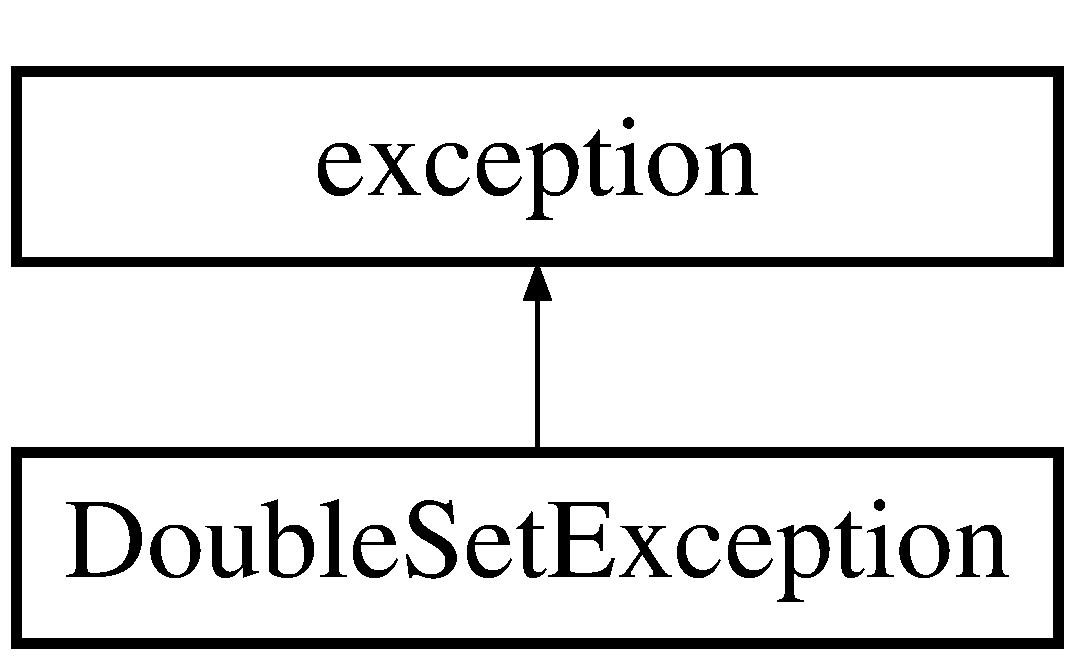
\includegraphics[height=2.000000cm]{structDoubleSetException}
\end{center}
\end{figure}
\subsection*{Public Member Functions}
\begin{DoxyCompactItemize}
\item 
\mbox{\Hypertarget{structDoubleSetException_a2568d6f42bcc8fb68ff83893eb4221b0}\label{structDoubleSetException_a2568d6f42bcc8fb68ff83893eb4221b0}} 
const char $\ast$ {\bfseries what} () const  throw ()
\end{DoxyCompactItemize}


The documentation for this struct was generated from the following file\+:\begin{DoxyCompactItemize}
\item 
/home/frederik/\+Dropbox/\+Astro/\+Magritte/src/\+Tools/set\+Once.\+hpp\end{DoxyCompactItemize}

\hypertarget{structFrequencies}{}\section{Frequencies Struct Reference}
\label{structFrequencies}\index{Frequencies@{Frequencies}}
\subsection*{Public Member Functions}
\begin{DoxyCompactItemize}
\item 
int \mbox{\hyperlink{structFrequencies_a0ca8d3fc3618359ac9630fbc0a99360f}{read}} (const \mbox{\hyperlink{structIo}{Io}} \&io, \mbox{\hyperlink{classParameters}{Parameters}} \&parameters)
\item 
int \mbox{\hyperlink{structFrequencies_a63d7282f4200d541b96279591312f22f}{write}} (const \mbox{\hyperlink{structIo}{Io}} \&io) const
\end{DoxyCompactItemize}
\subsection*{Public Attributes}
\begin{DoxyCompactItemize}
\item 
\mbox{\Hypertarget{structFrequencies_a330ed1d451b153a42191946acaee4ee0}\label{structFrequencies_a330ed1d451b153a42191946acaee4ee0}} 
v\+Real2 \mbox{\hyperlink{structFrequencies_a330ed1d451b153a42191946acaee4ee0}{nu}}
\begin{DoxyCompactList}\small\item\em \mbox{[}Hz\mbox{]} frequencies (ordered in f) (p,f) \end{DoxyCompactList}\item 
\mbox{\Hypertarget{structFrequencies_a643386df8be2d8edd40715fedfa4d061}\label{structFrequencies_a643386df8be2d8edd40715fedfa4d061}} 
Bool1 \mbox{\hyperlink{structFrequencies_a643386df8be2d8edd40715fedfa4d061}{appears\+\_\+in\+\_\+line\+\_\+integral}}
\begin{DoxyCompactList}\small\item\em True if the frequency appears in line integral. \end{DoxyCompactList}\item 
\mbox{\Hypertarget{structFrequencies_ac9b5a2b360373bd05660eff98ecd7774}\label{structFrequencies_ac9b5a2b360373bd05660eff98ecd7774}} 
Long1 \mbox{\hyperlink{structFrequencies_ac9b5a2b360373bd05660eff98ecd7774}{corresponding\+\_\+l\+\_\+for\+\_\+spec}}
\begin{DoxyCompactList}\small\item\em number of line species corresponding to frequency \end{DoxyCompactList}\item 
\mbox{\Hypertarget{structFrequencies_a34d7c5644fd7312eb41f8fc8680d74f6}\label{structFrequencies_a34d7c5644fd7312eb41f8fc8680d74f6}} 
Long1 \mbox{\hyperlink{structFrequencies_a34d7c5644fd7312eb41f8fc8680d74f6}{corresponding\+\_\+k\+\_\+for\+\_\+tran}}
\begin{DoxyCompactList}\small\item\em number of transition corresponding to frequency \end{DoxyCompactList}\item 
\mbox{\Hypertarget{structFrequencies_abf3f81ef858d0662098fb1aa2c61d1fa}\label{structFrequencies_abf3f81ef858d0662098fb1aa2c61d1fa}} 
Long1 \mbox{\hyperlink{structFrequencies_abf3f81ef858d0662098fb1aa2c61d1fa}{corresponding\+\_\+z\+\_\+for\+\_\+line}}
\begin{DoxyCompactList}\small\item\em number of line number corresponding to frequency \end{DoxyCompactList}\end{DoxyCompactItemize}


\subsection{Member Function Documentation}
\mbox{\Hypertarget{structFrequencies_a0ca8d3fc3618359ac9630fbc0a99360f}\label{structFrequencies_a0ca8d3fc3618359ac9630fbc0a99360f}} 
\index{Frequencies@{Frequencies}!read@{read}}
\index{read@{read}!Frequencies@{Frequencies}}
\subsubsection{\texorpdfstring{read()}{read()}}
{\footnotesize\ttfamily int Frequencies\+::read (\begin{DoxyParamCaption}\item[{const \mbox{\hyperlink{structIo}{Io}} \&}]{io,  }\item[{\mbox{\hyperlink{classParameters}{Parameters}} \&}]{parameters }\end{DoxyParamCaption})}

read\+: read in the data file 
\begin{DoxyParams}[1]{Parameters}
\mbox{\tt in}  & {\em io} & io object \\
\hline
\mbox{\tt in}  & {\em parameters} & model parameters object \\
\hline
\end{DoxyParams}
\mbox{\Hypertarget{structFrequencies_a63d7282f4200d541b96279591312f22f}\label{structFrequencies_a63d7282f4200d541b96279591312f22f}} 
\index{Frequencies@{Frequencies}!write@{write}}
\index{write@{write}!Frequencies@{Frequencies}}
\subsubsection{\texorpdfstring{write()}{write()}}
{\footnotesize\ttfamily int Frequencies\+::write (\begin{DoxyParamCaption}\item[{const \mbox{\hyperlink{structIo}{Io}} \&}]{io }\end{DoxyParamCaption}) const}

write\+: write out data structure 
\begin{DoxyParams}[1]{Parameters}
\mbox{\tt in}  & {\em io} & io object \\
\hline
\end{DoxyParams}


The documentation for this struct was generated from the following files\+:\begin{DoxyCompactItemize}
\item 
/home/frederik/\+Dropbox/\+Astro/\+Magritte/src/\+Model/\+Radiation/\+Frequencies/frequencies.\+hpp\item 
/home/frederik/\+Dropbox/\+Astro/\+Magritte/src/\+Model/\+Radiation/\+Frequencies/frequencies.\+cpp\end{DoxyCompactItemize}

\hypertarget{structGeometry}{}\section{Geometry Struct Reference}
\label{structGeometry}\index{Geometry@{Geometry}}


\mbox{\hyperlink{structGeometry}{Geometry}}\+: data structure containing all geometric data.  




{\ttfamily \#include $<$geometry.\+hpp$>$}

\subsection*{Public Member Functions}
\begin{DoxyCompactItemize}
\item 
int \mbox{\hyperlink{structGeometry_a129743f34789020e93923a15f85dcfc9}{read}} (const \mbox{\hyperlink{structIo}{Io}} \&io, \mbox{\hyperlink{classParameters}{Parameters}} \&parameters)
\item 
int \mbox{\hyperlink{structGeometry_a9cb010d7e27cdbdce9a552ad1e7ffa3c}{write}} (const \mbox{\hyperlink{structIo}{Io}} \&io) const
\item 
\mbox{\Hypertarget{structGeometry_ada5407ff5d7e2506061d8e3b535edbce}\label{structGeometry_ada5407ff5d7e2506061d8e3b535edbce}} 
Ray\+Data {\bfseries trace\+\_\+ray} (const long origin, const long ray, const double dshift\+\_\+max) const
\item 
\mbox{\Hypertarget{structGeometry_a83eaca7c81e577e6acceff613d8dda07}\label{structGeometry_a83eaca7c81e577e6acceff613d8dda07}} 
int {\bfseries set\+\_\+data} (const long crt, const long nxt, const double shift\+\_\+crt, const double shift\+\_\+nxt, const double d\+Z\+\_\+loc, const double dshift\+\_\+max, Ray\+Data \&ray\+Data) const
\item 
\mbox{\Hypertarget{structGeometry_a15635ef307c4a5cf3b5c94d2e9dd70ef}\label{structGeometry_a15635ef307c4a5cf3b5c94d2e9dd70ef}} 
long {\bfseries next} (const long origin, const long ray, const long current, double \&Z, double \&dZ) const
\item 
\mbox{\Hypertarget{structGeometry_a442e01e6c5b87939670ade6ae6836053}\label{structGeometry_a442e01e6c5b87939670ade6ae6836053}} 
double {\bfseries doppler\+\_\+shift} (const long origin, const long r, const long current) const
\end{DoxyCompactItemize}
\subsection*{Public Attributes}
\begin{DoxyCompactItemize}
\item 
\mbox{\Hypertarget{structGeometry_ab8fc1c31027c93d1e82f46111951966c}\label{structGeometry_ab8fc1c31027c93d1e82f46111951966c}} 
\mbox{\hyperlink{structCells}{Cells}} {\bfseries cells}
\item 
\mbox{\Hypertarget{structGeometry_ab40f75e6744eff6f8a04459cb5a770fa}\label{structGeometry_ab40f75e6744eff6f8a04459cb5a770fa}} 
\mbox{\hyperlink{structRays}{Rays}} {\bfseries rays}
\item 
\mbox{\Hypertarget{structGeometry_a9153b970abf6d0a7ac6074688c4833cc}\label{structGeometry_a9153b970abf6d0a7ac6074688c4833cc}} 
\mbox{\hyperlink{structBoundary}{Boundary}} {\bfseries boundary}
\item 
\mbox{\Hypertarget{structGeometry_ad66836932a465d3cb214d7a3d399c9d8}\label{structGeometry_ad66836932a465d3cb214d7a3d399c9d8}} 
\mbox{\hyperlink{structCameras}{Cameras}} {\bfseries cameras}
\end{DoxyCompactItemize}


\subsection{Detailed Description}
\mbox{\hyperlink{structGeometry}{Geometry}}\+: data structure containing all geometric data. 

\subsection{Member Function Documentation}
\mbox{\Hypertarget{structGeometry_a129743f34789020e93923a15f85dcfc9}\label{structGeometry_a129743f34789020e93923a15f85dcfc9}} 
\index{Geometry@{Geometry}!read@{read}}
\index{read@{read}!Geometry@{Geometry}}
\subsubsection{\texorpdfstring{read()}{read()}}
{\footnotesize\ttfamily int Geometry\+::read (\begin{DoxyParamCaption}\item[{const \mbox{\hyperlink{structIo}{Io}} \&}]{io,  }\item[{\mbox{\hyperlink{classParameters}{Parameters}} \&}]{parameters }\end{DoxyParamCaption})}

read\+: read the input into the data structure 
\begin{DoxyParams}[1]{Parameters}
\mbox{\tt in}  & {\em io} & io object \\
\hline
\mbox{\tt in}  & {\em parameters} & model parameters object \\
\hline
\end{DoxyParams}
\mbox{\Hypertarget{structGeometry_a9cb010d7e27cdbdce9a552ad1e7ffa3c}\label{structGeometry_a9cb010d7e27cdbdce9a552ad1e7ffa3c}} 
\index{Geometry@{Geometry}!write@{write}}
\index{write@{write}!Geometry@{Geometry}}
\subsubsection{\texorpdfstring{write()}{write()}}
{\footnotesize\ttfamily int Geometry\+::write (\begin{DoxyParamCaption}\item[{const \mbox{\hyperlink{structIo}{Io}} \&}]{io }\end{DoxyParamCaption}) const}

write\+: write the dat astructure 
\begin{DoxyParams}[1]{Parameters}
\mbox{\tt in}  & {\em io} & io object \\
\hline
\end{DoxyParams}


The documentation for this struct was generated from the following files\+:\begin{DoxyCompactItemize}
\item 
/home/frederik/\+Dropbox/\+Astro/\+Magritte/src/\+Model/\+Geometry/geometry.\+hpp\item 
/home/frederik/\+Dropbox/\+Astro/\+Magritte/src/\+Model/\+Geometry/geometry.\+cpp\end{DoxyCompactItemize}

\hypertarget{structGetBeforeSetException}{}\section{Get\+Before\+Set\+Exception Struct Reference}
\label{structGetBeforeSetException}\index{Get\+Before\+Set\+Exception@{Get\+Before\+Set\+Exception}}
Inheritance diagram for Get\+Before\+Set\+Exception\+:\begin{figure}[H]
\begin{center}
\leavevmode
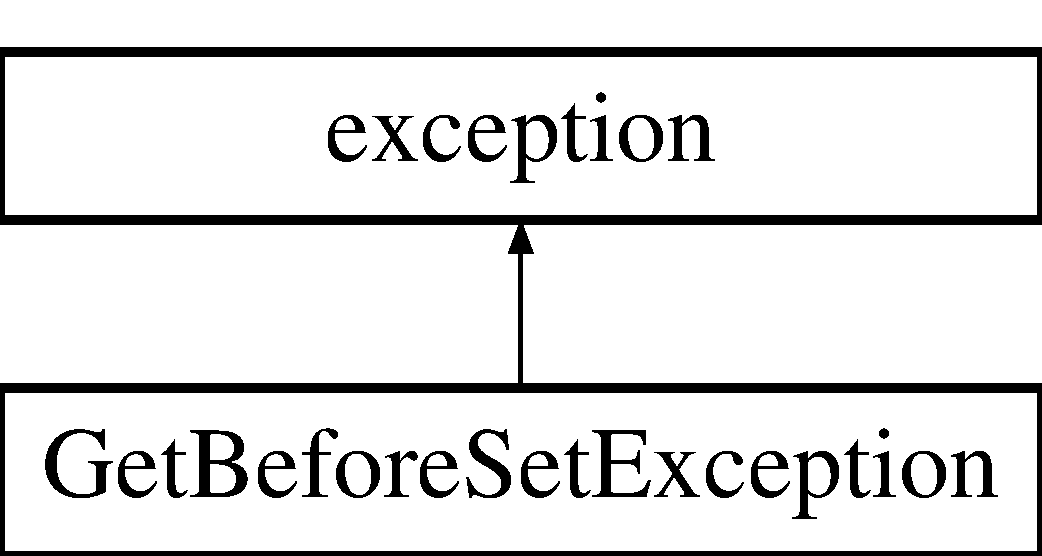
\includegraphics[height=2.000000cm]{structGetBeforeSetException}
\end{center}
\end{figure}
\subsection*{Public Member Functions}
\begin{DoxyCompactItemize}
\item 
\mbox{\Hypertarget{structGetBeforeSetException_aa0845c7c8351249d9a788b1b928f8ecb}\label{structGetBeforeSetException_aa0845c7c8351249d9a788b1b928f8ecb}} 
const char $\ast$ {\bfseries what} () const  throw ()
\end{DoxyCompactItemize}


The documentation for this struct was generated from the following file\+:\begin{DoxyCompactItemize}
\item 
/home/frederik/\+Dropbox/\+Astro/\+Magritte/src/\+Tools/set\+Once.\+hpp\end{DoxyCompactItemize}

\hypertarget{structImage}{}\section{Image Struct Reference}
\label{structImage}\index{Image@{Image}}


\mbox{\hyperlink{structImage}{Image}}\+: data structure for the images.  




{\ttfamily \#include $<$image.\+hpp$>$}

\subsection*{Public Member Functions}
\begin{DoxyCompactItemize}
\item 
\mbox{\Hypertarget{structImage_a20f4e6ffdb814623fa290d73bb1e797c}\label{structImage_a20f4e6ffdb814623fa290d73bb1e797c}} 
\mbox{\hyperlink{structImage_a20f4e6ffdb814623fa290d73bb1e797c}{Image}} (const long \mbox{\hyperlink{structImage_a96b20b62cef09709597a8c96559d0fa8}{ray\+\_\+nr}}, const \mbox{\hyperlink{classParameters}{Parameters}} \&parameters)
\begin{DoxyCompactList}\small\item\em Constructor for \mbox{\hyperlink{structImage}{Image}}. \end{DoxyCompactList}\item 
int \mbox{\hyperlink{structImage_a9b3922e23578e6e8f5f471c327c1b250}{write}} (const \mbox{\hyperlink{structIo}{Io}} \&io) const
\item 
\mbox{\Hypertarget{structImage_a9b5b0b4da304a0cebacabedfe9759c3e}\label{structImage_a9b5b0b4da304a0cebacabedfe9759c3e}} 
int \mbox{\hyperlink{structImage_a9b5b0b4da304a0cebacabedfe9759c3e}{set\+\_\+coordinates}} (const \mbox{\hyperlink{structGeometry}{Geometry}} \&geometry)
\begin{DoxyCompactList}\small\item\em set\+\_\+axis\+: set axis on which to project image \end{DoxyCompactList}\end{DoxyCompactItemize}
\subsection*{Public Attributes}
\begin{DoxyCompactItemize}
\item 
\mbox{\Hypertarget{structImage_a96b20b62cef09709597a8c96559d0fa8}\label{structImage_a96b20b62cef09709597a8c96559d0fa8}} 
const long \mbox{\hyperlink{structImage_a96b20b62cef09709597a8c96559d0fa8}{ray\+\_\+nr}}
\begin{DoxyCompactList}\small\item\em number of the ray to be imaged \end{DoxyCompactList}\item 
\mbox{\Hypertarget{structImage_affa6c57e43fdcde6839437377102a6e7}\label{structImage_affa6c57e43fdcde6839437377102a6e7}} 
Double1 \mbox{\hyperlink{structImage_affa6c57e43fdcde6839437377102a6e7}{ImX}}
\begin{DoxyCompactList}\small\item\em x coordinate of point in image \end{DoxyCompactList}\item 
\mbox{\Hypertarget{structImage_a99fe8443aa2bdd1e73421a1be071968c}\label{structImage_a99fe8443aa2bdd1e73421a1be071968c}} 
Double1 \mbox{\hyperlink{structImage_a99fe8443aa2bdd1e73421a1be071968c}{ImY}}
\begin{DoxyCompactList}\small\item\em y coordinate of point in image \end{DoxyCompactList}\item 
\mbox{\Hypertarget{structImage_aec73e9c458ec241940402be87de2cd12}\label{structImage_aec73e9c458ec241940402be87de2cd12}} 
Double2 \mbox{\hyperlink{structImage_aec73e9c458ec241940402be87de2cd12}{I\+\_\+p}}
\begin{DoxyCompactList}\small\item\em intensity out along ray (index(p,f)) \end{DoxyCompactList}\item 
\mbox{\Hypertarget{structImage_a3a4e1e82bb8a5855fe15b3ea49a1a188}\label{structImage_a3a4e1e82bb8a5855fe15b3ea49a1a188}} 
Double2 \mbox{\hyperlink{structImage_a3a4e1e82bb8a5855fe15b3ea49a1a188}{I\+\_\+m}}
\begin{DoxyCompactList}\small\item\em intensity out along ray (index(p,f)) \end{DoxyCompactList}\end{DoxyCompactItemize}


\subsection{Detailed Description}
\mbox{\hyperlink{structImage}{Image}}\+: data structure for the images. 

\subsection{Member Function Documentation}
\mbox{\Hypertarget{structImage_a9b3922e23578e6e8f5f471c327c1b250}\label{structImage_a9b3922e23578e6e8f5f471c327c1b250}} 
\index{Image@{Image}!write@{write}}
\index{write@{write}!Image@{Image}}
\subsubsection{\texorpdfstring{write()}{write()}}
{\footnotesize\ttfamily int Image\+::write (\begin{DoxyParamCaption}\item[{const \mbox{\hyperlink{structIo}{Io}} \&}]{io }\end{DoxyParamCaption}) const}

print\+: write out the images 
\begin{DoxyParams}[1]{Parameters}
\mbox{\tt in}  & {\em io} & io object \\
\hline
\end{DoxyParams}


The documentation for this struct was generated from the following files\+:\begin{DoxyCompactItemize}
\item 
/home/frederik/\+Dropbox/\+Astro/\+Magritte/src/\+Simulation/\+Image/image.\+hpp\item 
/home/frederik/\+Dropbox/\+Astro/\+Magritte/src/\+Simulation/\+Image/image.\+cpp\end{DoxyCompactItemize}

\hypertarget{structIo}{}\section{Io Struct Reference}
\label{structIo}\index{Io@{Io}}


\mbox{\hyperlink{structIo}{Io}}\+: Magritte\textquotesingle{}s input/output interface.  




{\ttfamily \#include $<$io.\+hpp$>$}

Inheritance diagram for Io\+:\begin{figure}[H]
\begin{center}
\leavevmode
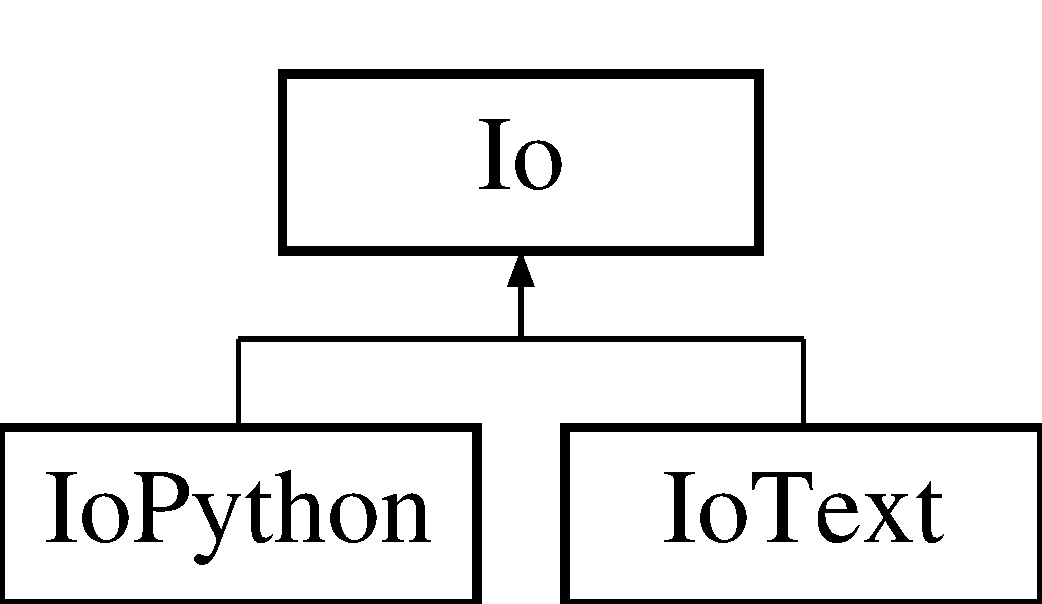
\includegraphics[height=2.000000cm]{structIo}
\end{center}
\end{figure}
\subsection*{Public Member Functions}
\begin{DoxyCompactItemize}
\item 
\mbox{\hyperlink{structIo_a5d9ad9b1887a715c69a8dce3e967f8d2}{Io}} (const string io\+\_\+file)
\item 
\mbox{\Hypertarget{structIo_a84c3a5705ee9fa5bd587ca62e1a264cb}\label{structIo_a84c3a5705ee9fa5bd587ca62e1a264cb}} 
virtual int {\bfseries read\+\_\+length} (const string fname, long \&length) const =0
\item 
\mbox{\Hypertarget{structIo_a83c506d5d17ea5cc29a2112230c2836d}\label{structIo_a83c506d5d17ea5cc29a2112230c2836d}} 
virtual int {\bfseries read\+\_\+width} (const string fname, long \&width) const =0
\item 
\mbox{\Hypertarget{structIo_aaf24fb114744f57fb2339496f943ce93}\label{structIo_aaf24fb114744f57fb2339496f943ce93}} 
virtual int {\bfseries read\+\_\+number} (const string fname, long \&number) const =0
\item 
\mbox{\Hypertarget{structIo_a163d88ee778a65ecafd62bcb35d9fc33}\label{structIo_a163d88ee778a65ecafd62bcb35d9fc33}} 
virtual int {\bfseries write\+\_\+number} (const string fname, const long \&number) const =0
\item 
\mbox{\Hypertarget{structIo_afa392b6b1b220976bcfc473540bbba40}\label{structIo_afa392b6b1b220976bcfc473540bbba40}} 
virtual int {\bfseries read\+\_\+number} (const string fname, double \&number) const =0
\item 
\mbox{\Hypertarget{structIo_ab68527fc3909f395e07564f0f726eeb7}\label{structIo_ab68527fc3909f395e07564f0f726eeb7}} 
virtual int {\bfseries write\+\_\+number} (const string fname, const double \&number) const =0
\item 
\mbox{\Hypertarget{structIo_ad5a50f54b41f5076b0b4fcc03ac0f270}\label{structIo_ad5a50f54b41f5076b0b4fcc03ac0f270}} 
virtual int {\bfseries read\+\_\+word} (const string fname, string \&word) const =0
\item 
\mbox{\Hypertarget{structIo_a60ce58b270dd4beeb0263bfdd2c63daf}\label{structIo_a60ce58b270dd4beeb0263bfdd2c63daf}} 
virtual int {\bfseries write\+\_\+word} (const string fname, const string \&word) const =0
\item 
\mbox{\Hypertarget{structIo_ad8db00e516c6686e4844c7ad6bfbd28e}\label{structIo_ad8db00e516c6686e4844c7ad6bfbd28e}} 
virtual int {\bfseries read\+\_\+list} (const string fname, Long1 \&list) const =0
\item 
\mbox{\Hypertarget{structIo_a88b9ed3d29a39626f53c5204757603d3}\label{structIo_a88b9ed3d29a39626f53c5204757603d3}} 
virtual int {\bfseries write\+\_\+list} (const string fname, const Long1 \&list) const =0
\item 
\mbox{\Hypertarget{structIo_aa1d905d1469000f40bfa03dfeca0de73}\label{structIo_aa1d905d1469000f40bfa03dfeca0de73}} 
virtual int {\bfseries read\+\_\+list} (const string fname, Double1 \&list) const =0
\item 
\mbox{\Hypertarget{structIo_ab0789472bdbe4f0b18e8497fe5773c45}\label{structIo_ab0789472bdbe4f0b18e8497fe5773c45}} 
virtual int {\bfseries write\+\_\+list} (const string fname, const Double1 \&list) const =0
\item 
\mbox{\Hypertarget{structIo_a292ce8e28c5c835354be4a5870aef70a}\label{structIo_a292ce8e28c5c835354be4a5870aef70a}} 
virtual int {\bfseries read\+\_\+list} (const string fname, String1 \&list) const =0
\item 
\mbox{\Hypertarget{structIo_a9a0f1f37f414d4f8480878aef4a7a859}\label{structIo_a9a0f1f37f414d4f8480878aef4a7a859}} 
virtual int {\bfseries write\+\_\+list} (const string fname, const String1 \&list) const =0
\item 
\mbox{\Hypertarget{structIo_af6cacc007e010a226459b37ba976aa18}\label{structIo_af6cacc007e010a226459b37ba976aa18}} 
virtual int {\bfseries read\+\_\+array} (const string fname, Long2 \&array) const =0
\item 
\mbox{\Hypertarget{structIo_aa73fe79d27fbaf31cbea124769e13a2e}\label{structIo_aa73fe79d27fbaf31cbea124769e13a2e}} 
virtual int {\bfseries write\+\_\+array} (const string fname, const Long2 \&array) const =0
\item 
\mbox{\Hypertarget{structIo_a4b1c5f54037a18b97c47c2fc35bbfb1d}\label{structIo_a4b1c5f54037a18b97c47c2fc35bbfb1d}} 
virtual int {\bfseries read\+\_\+array} (const string fname, Double2 \&array) const =0
\item 
\mbox{\Hypertarget{structIo_af2f52ba6b21d23af0b3bed255e815c5b}\label{structIo_af2f52ba6b21d23af0b3bed255e815c5b}} 
virtual int {\bfseries write\+\_\+array} (const string fname, const Double2 \&array) const =0
\item 
\mbox{\Hypertarget{structIo_aef5a70d68049574861ebbd40aea9b293}\label{structIo_aef5a70d68049574861ebbd40aea9b293}} 
virtual int {\bfseries read\+\_\+3\+\_\+vector} (const string fname, Double1 \&x, Double1 \&y, Double1 \&z) const =0
\item 
\mbox{\Hypertarget{structIo_a175931043244e44f87641ea7c5c7aeff}\label{structIo_a175931043244e44f87641ea7c5c7aeff}} 
virtual int {\bfseries write\+\_\+3\+\_\+vector} (const string fname, const Double1 \&x, const Double1 \&y, const Double1 \&z) const =0
\end{DoxyCompactItemize}
\subsection*{Public Attributes}
\begin{DoxyCompactItemize}
\item 
\mbox{\Hypertarget{structIo_ad39461ed5b16c4fa74363a2a593d12e3}\label{structIo_ad39461ed5b16c4fa74363a2a593d12e3}} 
const string {\bfseries io\+\_\+file}
\end{DoxyCompactItemize}


\subsection{Detailed Description}
\mbox{\hyperlink{structIo}{Io}}\+: Magritte\textquotesingle{}s input/output interface. 

\subsection{Constructor \& Destructor Documentation}
\mbox{\Hypertarget{structIo_a5d9ad9b1887a715c69a8dce3e967f8d2}\label{structIo_a5d9ad9b1887a715c69a8dce3e967f8d2}} 
\index{Io@{Io}!Io@{Io}}
\index{Io@{Io}!Io@{Io}}
\subsubsection{\texorpdfstring{Io()}{Io()}}
{\footnotesize\ttfamily Io\+::\+Io (\begin{DoxyParamCaption}\item[{const string}]{io\+\_\+file }\end{DoxyParamCaption})}

Constructor for \mbox{\hyperlink{structIo}{Io}} 
\begin{DoxyParams}[1]{Parameters}
\mbox{\tt in}  & {\em io\+\_\+file} & file to read from and write to \\
\hline
\end{DoxyParams}


The documentation for this struct was generated from the following files\+:\begin{DoxyCompactItemize}
\item 
/home/frederik/\+Dropbox/\+Astro/\+Magritte/src/\+Io/io.\+hpp\item 
/home/frederik/\+Dropbox/\+Astro/\+Magritte/src/\+Io/io.\+cpp\end{DoxyCompactItemize}

\hypertarget{structIoPython}{}\section{Io\+Python Struct Reference}
\label{structIoPython}\index{Io\+Python@{Io\+Python}}


\mbox{\hyperlink{structIoText}{Io\+Text}}\+: io specified by text files.  




{\ttfamily \#include $<$io\+\_\+python.\+hpp$>$}

Inheritance diagram for Io\+Python\+:\begin{figure}[H]
\begin{center}
\leavevmode
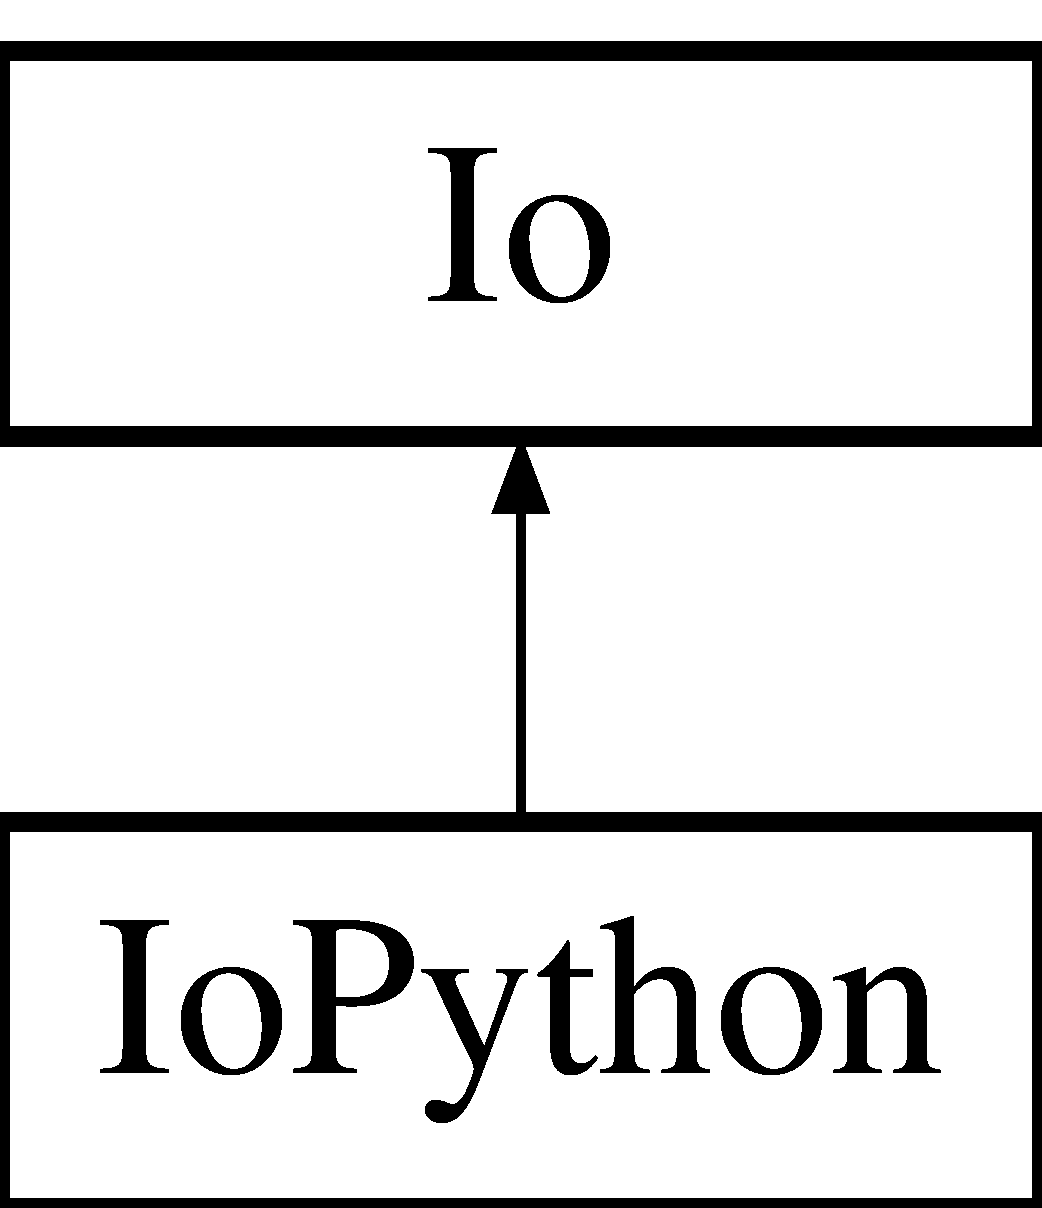
\includegraphics[height=2.000000cm]{structIoPython}
\end{center}
\end{figure}
\subsection*{Public Member Functions}
\begin{DoxyCompactItemize}
\item 
\mbox{\hyperlink{structIoPython_aecfbf8a5a148d102ab584493c7b32477}{Io\+Python}} (const string implementation, const string io\+\_\+file)
\item 
int \mbox{\hyperlink{structIoPython_a0317edc1965de95540713f96300b5fa3}{read\+\_\+length}} (const string fname, long \&length) const
\item 
int \mbox{\hyperlink{structIoPython_a8d0cf7e49496f8393a6c975d8091ee32}{read\+\_\+width}} (const string fname, long \&width) const
\item 
int \mbox{\hyperlink{structIoPython_a181ebe01e99ff21c617dadd43df1c79a}{read\+\_\+number}} (const string fname, long \&number) const
\item 
int \mbox{\hyperlink{structIoPython_acbdb2e4c9bfaeae992572462a6f27538}{write\+\_\+number}} (const string fname, const long \&number) const
\item 
int \mbox{\hyperlink{structIoPython_a601a92b585dda826191bfaabdb11dc81}{read\+\_\+number}} (const string fname, double \&number) const
\item 
int \mbox{\hyperlink{structIoPython_aa1088aef56bd86c4a986460a39e4c3dd}{write\+\_\+number}} (const string fname, const double \&number) const
\item 
int \mbox{\hyperlink{structIoPython_a3de76956d06bbdc6daf93dfb2422ac8a}{read\+\_\+word}} (const string fname, string \&word) const
\item 
int \mbox{\hyperlink{structIoPython_ae9f8fda0e13b5a23923451f83328e00b}{write\+\_\+word}} (const string fname, const string \&word) const
\item 
int \mbox{\hyperlink{structIoPython_a2ebe407ec2594d63cb496a296dab422d}{read\+\_\+list}} (const string fname, Long1 \&list) const
\item 
int \mbox{\hyperlink{structIoPython_a362806b2c79cfd2710bb6aa5abdad81c}{write\+\_\+list}} (const string fname, const Long1 \&list) const
\item 
int \mbox{\hyperlink{structIoPython_ac4e86a5720764c24176c8dce65ff86f3}{read\+\_\+list}} (const string fname, Double1 \&list) const
\item 
int \mbox{\hyperlink{structIoPython_aef1a23954e7bfb682237f2c9c4278b59}{write\+\_\+list}} (const string fname, const Double1 \&list) const
\item 
int \mbox{\hyperlink{structIoPython_a924ffac9eca892940d1dd91cd97a6be3}{read\+\_\+list}} (const string fname, String1 \&list) const
\item 
int \mbox{\hyperlink{structIoPython_aa8657964ce2051a963614d6f54578a7b}{write\+\_\+list}} (const string fname, const String1 \&list) const
\item 
int \mbox{\hyperlink{structIoPython_ad37c12b459683395fdcb63be94352c60}{read\+\_\+array}} (const string fname, Long2 \&array) const
\item 
int \mbox{\hyperlink{structIoPython_aaa819900c69a39611ac7e2e46598f6bb}{write\+\_\+array}} (const string fname, const Long2 \&array) const
\item 
int \mbox{\hyperlink{structIoPython_a0000f072ed7e6744c222f215701c219e}{read\+\_\+array}} (const string fname, Double2 \&array) const
\item 
int \mbox{\hyperlink{structIoPython_a2c5827350f08648843d06734b38276c3}{write\+\_\+array}} (const string fname, const Double2 \&array) const
\item 
int \mbox{\hyperlink{structIoPython_a7f9224586baa4e837e55e3f3b1eac85d}{read\+\_\+3\+\_\+vector}} (const string fname, Double1 \&x, Double1 \&y, Double1 \&z) const
\item 
int \mbox{\hyperlink{structIoPython_a90a56f09b1e1873274b20e42386a420f}{write\+\_\+3\+\_\+vector}} (const string fname, const Double1 \&x, const Double1 \&y, const Double1 \&z) const
\end{DoxyCompactItemize}
\subsection*{Public Attributes}
\begin{DoxyCompactItemize}
\item 
\mbox{\Hypertarget{structIoPython_ad0a9ece7b694753a335fe99792741cba}\label{structIoPython_ad0a9ece7b694753a335fe99792741cba}} 
const string {\bfseries implementation}
\end{DoxyCompactItemize}


\subsection{Detailed Description}
\mbox{\hyperlink{structIoText}{Io\+Text}}\+: io specified by text files. 

\subsection{Constructor \& Destructor Documentation}
\mbox{\Hypertarget{structIoPython_aecfbf8a5a148d102ab584493c7b32477}\label{structIoPython_aecfbf8a5a148d102ab584493c7b32477}} 
\index{Io\+Python@{Io\+Python}!Io\+Python@{Io\+Python}}
\index{Io\+Python@{Io\+Python}!Io\+Python@{Io\+Python}}
\subsubsection{\texorpdfstring{Io\+Python()}{IoPython()}}
{\footnotesize\ttfamily Io\+Python\+::\+Io\+Python (\begin{DoxyParamCaption}\item[{const string}]{imp,  }\item[{const string}]{io\+\_\+file }\end{DoxyParamCaption})}

Constructor for \mbox{\hyperlink{structIoPython}{Io\+Python}} 
\begin{DoxyParams}[1]{Parameters}
\mbox{\tt in}  & {\em implementation} & python module containing the implementaion \\
\hline
\mbox{\tt in}  & {\em io\+\_\+file} & file to read from and write to \\
\hline
\end{DoxyParams}


\subsection{Member Function Documentation}
\mbox{\Hypertarget{structIoPython_a7f9224586baa4e837e55e3f3b1eac85d}\label{structIoPython_a7f9224586baa4e837e55e3f3b1eac85d}} 
\index{Io\+Python@{Io\+Python}!read\+\_\+3\+\_\+vector@{read\+\_\+3\+\_\+vector}}
\index{read\+\_\+3\+\_\+vector@{read\+\_\+3\+\_\+vector}!Io\+Python@{Io\+Python}}
\subsubsection{\texorpdfstring{read\+\_\+3\+\_\+vector()}{read\_3\_vector()}}
{\footnotesize\ttfamily int Io\+Python\+::read\+\_\+3\+\_\+vector (\begin{DoxyParamCaption}\item[{const string}]{file\+\_\+name,  }\item[{Double1 \&}]{x,  }\item[{Double1 \&}]{y,  }\item[{Double1 \&}]{z }\end{DoxyParamCaption}) const\hspace{0.3cm}{\ttfamily [virtual]}}

read\+\_\+3\+\_\+vector\+: 
\begin{DoxyParams}[1]{Parameters}
\mbox{\tt in}  & {\em file\+\_\+name} & path to file containing the data \\
\hline
\mbox{\tt in}  & {\em x} & x component of the vector to be read \\
\hline
\mbox{\tt in}  & {\em y} & y component of the vector to be read \\
\hline
\mbox{\tt in}  & {\em z} & z component of the vector to be read \\
\hline
\end{DoxyParams}


Implements \mbox{\hyperlink{structIo}{Io}}.

\mbox{\Hypertarget{structIoPython_ad37c12b459683395fdcb63be94352c60}\label{structIoPython_ad37c12b459683395fdcb63be94352c60}} 
\index{Io\+Python@{Io\+Python}!read\+\_\+array@{read\+\_\+array}}
\index{read\+\_\+array@{read\+\_\+array}!Io\+Python@{Io\+Python}}
\subsubsection{\texorpdfstring{read\+\_\+array()}{read\_array()}\hspace{0.1cm}{\footnotesize\ttfamily [1/2]}}
{\footnotesize\ttfamily int Io\+Python\+::read\+\_\+array (\begin{DoxyParamCaption}\item[{const string}]{file\+\_\+name,  }\item[{Long2 \&}]{array }\end{DoxyParamCaption}) const\hspace{0.3cm}{\ttfamily [virtual]}}

read\+\_\+array\+: 
\begin{DoxyParams}[1]{Parameters}
\mbox{\tt in}  & {\em file\+\_\+name} & path to file containing the data \\
\hline
\mbox{\tt in}  & {\em list} & array to be filled \\
\hline
\end{DoxyParams}


Implements \mbox{\hyperlink{structIo}{Io}}.

\mbox{\Hypertarget{structIoPython_a0000f072ed7e6744c222f215701c219e}\label{structIoPython_a0000f072ed7e6744c222f215701c219e}} 
\index{Io\+Python@{Io\+Python}!read\+\_\+array@{read\+\_\+array}}
\index{read\+\_\+array@{read\+\_\+array}!Io\+Python@{Io\+Python}}
\subsubsection{\texorpdfstring{read\+\_\+array()}{read\_array()}\hspace{0.1cm}{\footnotesize\ttfamily [2/2]}}
{\footnotesize\ttfamily int Io\+Python\+::read\+\_\+array (\begin{DoxyParamCaption}\item[{const string}]{file\+\_\+name,  }\item[{Double2 \&}]{array }\end{DoxyParamCaption}) const\hspace{0.3cm}{\ttfamily [virtual]}}

read\+\_\+array\+: 
\begin{DoxyParams}[1]{Parameters}
\mbox{\tt in}  & {\em file\+\_\+name} & path to file containing the data \\
\hline
\mbox{\tt in}  & {\em list} & array to be filled \\
\hline
\end{DoxyParams}


Implements \mbox{\hyperlink{structIo}{Io}}.

\mbox{\Hypertarget{structIoPython_a0317edc1965de95540713f96300b5fa3}\label{structIoPython_a0317edc1965de95540713f96300b5fa3}} 
\index{Io\+Python@{Io\+Python}!read\+\_\+length@{read\+\_\+length}}
\index{read\+\_\+length@{read\+\_\+length}!Io\+Python@{Io\+Python}}
\subsubsection{\texorpdfstring{read\+\_\+length()}{read\_length()}}
{\footnotesize\ttfamily int Io\+Python\+::read\+\_\+length (\begin{DoxyParamCaption}\item[{const string}]{file\+\_\+name,  }\item[{long \&}]{length }\end{DoxyParamCaption}) const\hspace{0.3cm}{\ttfamily [virtual]}}

read\+\_\+length\+: 
\begin{DoxyParams}[1]{Parameters}
\mbox{\tt in}  & {\em file\+\_\+name} & path to file containing the data \\
\hline
\mbox{\tt out}  & {\em length} & length to be read \\
\hline
\end{DoxyParams}


Implements \mbox{\hyperlink{structIo}{Io}}.

\mbox{\Hypertarget{structIoPython_a2ebe407ec2594d63cb496a296dab422d}\label{structIoPython_a2ebe407ec2594d63cb496a296dab422d}} 
\index{Io\+Python@{Io\+Python}!read\+\_\+list@{read\+\_\+list}}
\index{read\+\_\+list@{read\+\_\+list}!Io\+Python@{Io\+Python}}
\subsubsection{\texorpdfstring{read\+\_\+list()}{read\_list()}\hspace{0.1cm}{\footnotesize\ttfamily [1/3]}}
{\footnotesize\ttfamily int Io\+Python\+::read\+\_\+list (\begin{DoxyParamCaption}\item[{const string}]{file\+\_\+name,  }\item[{Long1 \&}]{list }\end{DoxyParamCaption}) const\hspace{0.3cm}{\ttfamily [virtual]}}

read\+\_\+list\+: 
\begin{DoxyParams}[1]{Parameters}
\mbox{\tt in}  & {\em file\+\_\+name} & path to file containing the data \\
\hline
\mbox{\tt in}  & {\em list} & list to be filled \\
\hline
\end{DoxyParams}


Implements \mbox{\hyperlink{structIo}{Io}}.

\mbox{\Hypertarget{structIoPython_ac4e86a5720764c24176c8dce65ff86f3}\label{structIoPython_ac4e86a5720764c24176c8dce65ff86f3}} 
\index{Io\+Python@{Io\+Python}!read\+\_\+list@{read\+\_\+list}}
\index{read\+\_\+list@{read\+\_\+list}!Io\+Python@{Io\+Python}}
\subsubsection{\texorpdfstring{read\+\_\+list()}{read\_list()}\hspace{0.1cm}{\footnotesize\ttfamily [2/3]}}
{\footnotesize\ttfamily int Io\+Python\+::read\+\_\+list (\begin{DoxyParamCaption}\item[{const string}]{file\+\_\+name,  }\item[{Double1 \&}]{list }\end{DoxyParamCaption}) const\hspace{0.3cm}{\ttfamily [virtual]}}

read\+\_\+list\+: 
\begin{DoxyParams}[1]{Parameters}
\mbox{\tt in}  & {\em file\+\_\+name} & path to file containing the data \\
\hline
\mbox{\tt in}  & {\em list} & list to be filled \\
\hline
\end{DoxyParams}


Implements \mbox{\hyperlink{structIo}{Io}}.

\mbox{\Hypertarget{structIoPython_a924ffac9eca892940d1dd91cd97a6be3}\label{structIoPython_a924ffac9eca892940d1dd91cd97a6be3}} 
\index{Io\+Python@{Io\+Python}!read\+\_\+list@{read\+\_\+list}}
\index{read\+\_\+list@{read\+\_\+list}!Io\+Python@{Io\+Python}}
\subsubsection{\texorpdfstring{read\+\_\+list()}{read\_list()}\hspace{0.1cm}{\footnotesize\ttfamily [3/3]}}
{\footnotesize\ttfamily int Io\+Python\+::read\+\_\+list (\begin{DoxyParamCaption}\item[{const string}]{file\+\_\+name,  }\item[{String1 \&}]{list }\end{DoxyParamCaption}) const\hspace{0.3cm}{\ttfamily [virtual]}}

read\+\_\+list\+: 
\begin{DoxyParams}[1]{Parameters}
\mbox{\tt in}  & {\em file\+\_\+name} & path to file containing the data \\
\hline
\mbox{\tt in}  & {\em list} & list to be filled \\
\hline
\end{DoxyParams}


Implements \mbox{\hyperlink{structIo}{Io}}.

\mbox{\Hypertarget{structIoPython_a181ebe01e99ff21c617dadd43df1c79a}\label{structIoPython_a181ebe01e99ff21c617dadd43df1c79a}} 
\index{Io\+Python@{Io\+Python}!read\+\_\+number@{read\+\_\+number}}
\index{read\+\_\+number@{read\+\_\+number}!Io\+Python@{Io\+Python}}
\subsubsection{\texorpdfstring{read\+\_\+number()}{read\_number()}\hspace{0.1cm}{\footnotesize\ttfamily [1/2]}}
{\footnotesize\ttfamily int Io\+Python\+::read\+\_\+number (\begin{DoxyParamCaption}\item[{const string}]{file\+\_\+name,  }\item[{long \&}]{number }\end{DoxyParamCaption}) const\hspace{0.3cm}{\ttfamily [virtual]}}

read\+\_\+number\+: 
\begin{DoxyParams}[1]{Parameters}
\mbox{\tt in}  & {\em file\+\_\+name} & file containing the number \\
\hline
\mbox{\tt out}  & {\em number} & number to be read \\
\hline
\end{DoxyParams}


Implements \mbox{\hyperlink{structIo}{Io}}.

\mbox{\Hypertarget{structIoPython_a601a92b585dda826191bfaabdb11dc81}\label{structIoPython_a601a92b585dda826191bfaabdb11dc81}} 
\index{Io\+Python@{Io\+Python}!read\+\_\+number@{read\+\_\+number}}
\index{read\+\_\+number@{read\+\_\+number}!Io\+Python@{Io\+Python}}
\subsubsection{\texorpdfstring{read\+\_\+number()}{read\_number()}\hspace{0.1cm}{\footnotesize\ttfamily [2/2]}}
{\footnotesize\ttfamily int Io\+Python\+::read\+\_\+number (\begin{DoxyParamCaption}\item[{const string}]{file\+\_\+name,  }\item[{double \&}]{number }\end{DoxyParamCaption}) const\hspace{0.3cm}{\ttfamily [virtual]}}

read\+\_\+number\+: 
\begin{DoxyParams}[1]{Parameters}
\mbox{\tt in}  & {\em file\+\_\+name} & file containing the number \\
\hline
\mbox{\tt out}  & {\em number} & number to be read \\
\hline
\end{DoxyParams}


Implements \mbox{\hyperlink{structIo}{Io}}.

\mbox{\Hypertarget{structIoPython_a8d0cf7e49496f8393a6c975d8091ee32}\label{structIoPython_a8d0cf7e49496f8393a6c975d8091ee32}} 
\index{Io\+Python@{Io\+Python}!read\+\_\+width@{read\+\_\+width}}
\index{read\+\_\+width@{read\+\_\+width}!Io\+Python@{Io\+Python}}
\subsubsection{\texorpdfstring{read\+\_\+width()}{read\_width()}}
{\footnotesize\ttfamily int Io\+Python\+::read\+\_\+width (\begin{DoxyParamCaption}\item[{const string}]{file\+\_\+name,  }\item[{long \&}]{length }\end{DoxyParamCaption}) const\hspace{0.3cm}{\ttfamily [virtual]}}

read\+\_\+width\+: 
\begin{DoxyParams}[1]{Parameters}
\mbox{\tt in}  & {\em file\+\_\+name} & path to file containing the data \\
\hline
\mbox{\tt out}  & {\em length} & length to be read \\
\hline
\end{DoxyParams}


Implements \mbox{\hyperlink{structIo}{Io}}.

\mbox{\Hypertarget{structIoPython_a3de76956d06bbdc6daf93dfb2422ac8a}\label{structIoPython_a3de76956d06bbdc6daf93dfb2422ac8a}} 
\index{Io\+Python@{Io\+Python}!read\+\_\+word@{read\+\_\+word}}
\index{read\+\_\+word@{read\+\_\+word}!Io\+Python@{Io\+Python}}
\subsubsection{\texorpdfstring{read\+\_\+word()}{read\_word()}}
{\footnotesize\ttfamily int Io\+Python\+::read\+\_\+word (\begin{DoxyParamCaption}\item[{const string}]{file\+\_\+name,  }\item[{string \&}]{word }\end{DoxyParamCaption}) const\hspace{0.3cm}{\ttfamily [virtual]}}

read\+\_\+word\+: 
\begin{DoxyParams}[1]{Parameters}
\mbox{\tt in}  & {\em file\+\_\+name} & file containing the number \\
\hline
\mbox{\tt out}  & {\em word} & word to be written \\
\hline
\end{DoxyParams}


Implements \mbox{\hyperlink{structIo}{Io}}.

\mbox{\Hypertarget{structIoPython_a90a56f09b1e1873274b20e42386a420f}\label{structIoPython_a90a56f09b1e1873274b20e42386a420f}} 
\index{Io\+Python@{Io\+Python}!write\+\_\+3\+\_\+vector@{write\+\_\+3\+\_\+vector}}
\index{write\+\_\+3\+\_\+vector@{write\+\_\+3\+\_\+vector}!Io\+Python@{Io\+Python}}
\subsubsection{\texorpdfstring{write\+\_\+3\+\_\+vector()}{write\_3\_vector()}}
{\footnotesize\ttfamily int Io\+Python\+::write\+\_\+3\+\_\+vector (\begin{DoxyParamCaption}\item[{const string}]{file\+\_\+name,  }\item[{const Double1 \&}]{x,  }\item[{const Double1 \&}]{y,  }\item[{const Double1 \&}]{z }\end{DoxyParamCaption}) const\hspace{0.3cm}{\ttfamily [virtual]}}

write\+\_\+3\+\_\+vector\+: 
\begin{DoxyParams}[1]{Parameters}
\mbox{\tt in}  & {\em file\+\_\+name} & path to file containing the data \\
\hline
\mbox{\tt in}  & {\em x} & x component of the vector to be written \\
\hline
\mbox{\tt in}  & {\em y} & y component of the vector to be written \\
\hline
\mbox{\tt in}  & {\em z} & z component of the vector to be written \\
\hline
\end{DoxyParams}


Implements \mbox{\hyperlink{structIo}{Io}}.

\mbox{\Hypertarget{structIoPython_aaa819900c69a39611ac7e2e46598f6bb}\label{structIoPython_aaa819900c69a39611ac7e2e46598f6bb}} 
\index{Io\+Python@{Io\+Python}!write\+\_\+array@{write\+\_\+array}}
\index{write\+\_\+array@{write\+\_\+array}!Io\+Python@{Io\+Python}}
\subsubsection{\texorpdfstring{write\+\_\+array()}{write\_array()}\hspace{0.1cm}{\footnotesize\ttfamily [1/2]}}
{\footnotesize\ttfamily int Io\+Python\+::write\+\_\+array (\begin{DoxyParamCaption}\item[{const string}]{file\+\_\+name,  }\item[{const Long2 \&}]{array }\end{DoxyParamCaption}) const\hspace{0.3cm}{\ttfamily [virtual]}}

write\+\_\+array\+: 
\begin{DoxyParams}[1]{Parameters}
\mbox{\tt in}  & {\em file\+\_\+name} & path to file containing the data \\
\hline
\mbox{\tt in}  & {\em list} & array to be written \\
\hline
\end{DoxyParams}


Implements \mbox{\hyperlink{structIo}{Io}}.

\mbox{\Hypertarget{structIoPython_a2c5827350f08648843d06734b38276c3}\label{structIoPython_a2c5827350f08648843d06734b38276c3}} 
\index{Io\+Python@{Io\+Python}!write\+\_\+array@{write\+\_\+array}}
\index{write\+\_\+array@{write\+\_\+array}!Io\+Python@{Io\+Python}}
\subsubsection{\texorpdfstring{write\+\_\+array()}{write\_array()}\hspace{0.1cm}{\footnotesize\ttfamily [2/2]}}
{\footnotesize\ttfamily int Io\+Python\+::write\+\_\+array (\begin{DoxyParamCaption}\item[{const string}]{file\+\_\+name,  }\item[{const Double2 \&}]{array }\end{DoxyParamCaption}) const\hspace{0.3cm}{\ttfamily [virtual]}}

write\+\_\+array\+: 
\begin{DoxyParams}[1]{Parameters}
\mbox{\tt in}  & {\em file\+\_\+name} & path to file containing the data \\
\hline
\mbox{\tt in}  & {\em list} & array to be written \\
\hline
\end{DoxyParams}


Implements \mbox{\hyperlink{structIo}{Io}}.

\mbox{\Hypertarget{structIoPython_a362806b2c79cfd2710bb6aa5abdad81c}\label{structIoPython_a362806b2c79cfd2710bb6aa5abdad81c}} 
\index{Io\+Python@{Io\+Python}!write\+\_\+list@{write\+\_\+list}}
\index{write\+\_\+list@{write\+\_\+list}!Io\+Python@{Io\+Python}}
\subsubsection{\texorpdfstring{write\+\_\+list()}{write\_list()}\hspace{0.1cm}{\footnotesize\ttfamily [1/3]}}
{\footnotesize\ttfamily int Io\+Python\+::write\+\_\+list (\begin{DoxyParamCaption}\item[{const string}]{file\+\_\+name,  }\item[{const Long1 \&}]{list }\end{DoxyParamCaption}) const\hspace{0.3cm}{\ttfamily [virtual]}}

write\+\_\+list\+: 
\begin{DoxyParams}[1]{Parameters}
\mbox{\tt in}  & {\em file\+\_\+name} & path to file containing the data \\
\hline
\mbox{\tt in}  & {\em list} & list to be written \\
\hline
\end{DoxyParams}


Implements \mbox{\hyperlink{structIo}{Io}}.

\mbox{\Hypertarget{structIoPython_aef1a23954e7bfb682237f2c9c4278b59}\label{structIoPython_aef1a23954e7bfb682237f2c9c4278b59}} 
\index{Io\+Python@{Io\+Python}!write\+\_\+list@{write\+\_\+list}}
\index{write\+\_\+list@{write\+\_\+list}!Io\+Python@{Io\+Python}}
\subsubsection{\texorpdfstring{write\+\_\+list()}{write\_list()}\hspace{0.1cm}{\footnotesize\ttfamily [2/3]}}
{\footnotesize\ttfamily int Io\+Python\+::write\+\_\+list (\begin{DoxyParamCaption}\item[{const string}]{file\+\_\+name,  }\item[{const Double1 \&}]{list }\end{DoxyParamCaption}) const\hspace{0.3cm}{\ttfamily [virtual]}}

write\+\_\+list\+: 
\begin{DoxyParams}[1]{Parameters}
\mbox{\tt in}  & {\em file\+\_\+name} & path to file containing the data \\
\hline
\mbox{\tt in}  & {\em list} & list to be written \\
\hline
\end{DoxyParams}


Implements \mbox{\hyperlink{structIo}{Io}}.

\mbox{\Hypertarget{structIoPython_aa8657964ce2051a963614d6f54578a7b}\label{structIoPython_aa8657964ce2051a963614d6f54578a7b}} 
\index{Io\+Python@{Io\+Python}!write\+\_\+list@{write\+\_\+list}}
\index{write\+\_\+list@{write\+\_\+list}!Io\+Python@{Io\+Python}}
\subsubsection{\texorpdfstring{write\+\_\+list()}{write\_list()}\hspace{0.1cm}{\footnotesize\ttfamily [3/3]}}
{\footnotesize\ttfamily int Io\+Python\+::write\+\_\+list (\begin{DoxyParamCaption}\item[{const string}]{file\+\_\+name,  }\item[{const String1 \&}]{list }\end{DoxyParamCaption}) const\hspace{0.3cm}{\ttfamily [virtual]}}

write\+\_\+list\+: 
\begin{DoxyParams}[1]{Parameters}
\mbox{\tt in}  & {\em file\+\_\+name} & path to file containing the data \\
\hline
\mbox{\tt in}  & {\em list} & list to be written \\
\hline
\end{DoxyParams}


Implements \mbox{\hyperlink{structIo}{Io}}.

\mbox{\Hypertarget{structIoPython_acbdb2e4c9bfaeae992572462a6f27538}\label{structIoPython_acbdb2e4c9bfaeae992572462a6f27538}} 
\index{Io\+Python@{Io\+Python}!write\+\_\+number@{write\+\_\+number}}
\index{write\+\_\+number@{write\+\_\+number}!Io\+Python@{Io\+Python}}
\subsubsection{\texorpdfstring{write\+\_\+number()}{write\_number()}\hspace{0.1cm}{\footnotesize\ttfamily [1/2]}}
{\footnotesize\ttfamily int Io\+Python\+::write\+\_\+number (\begin{DoxyParamCaption}\item[{const string}]{file\+\_\+name,  }\item[{const long \&}]{number }\end{DoxyParamCaption}) const\hspace{0.3cm}{\ttfamily [virtual]}}

write\+\_\+number\+: 
\begin{DoxyParams}[1]{Parameters}
\mbox{\tt in}  & {\em file\+\_\+name} & file containing the number \\
\hline
\mbox{\tt in}  & {\em number} & number to be written \\
\hline
\end{DoxyParams}


Implements \mbox{\hyperlink{structIo}{Io}}.

\mbox{\Hypertarget{structIoPython_aa1088aef56bd86c4a986460a39e4c3dd}\label{structIoPython_aa1088aef56bd86c4a986460a39e4c3dd}} 
\index{Io\+Python@{Io\+Python}!write\+\_\+number@{write\+\_\+number}}
\index{write\+\_\+number@{write\+\_\+number}!Io\+Python@{Io\+Python}}
\subsubsection{\texorpdfstring{write\+\_\+number()}{write\_number()}\hspace{0.1cm}{\footnotesize\ttfamily [2/2]}}
{\footnotesize\ttfamily int Io\+Python\+::write\+\_\+number (\begin{DoxyParamCaption}\item[{const string}]{file\+\_\+name,  }\item[{const double \&}]{number }\end{DoxyParamCaption}) const\hspace{0.3cm}{\ttfamily [virtual]}}

write\+\_\+number\+: 
\begin{DoxyParams}[1]{Parameters}
\mbox{\tt in}  & {\em file\+\_\+name} & file containing the number \\
\hline
\mbox{\tt in}  & {\em number} & number to be written \\
\hline
\end{DoxyParams}


Implements \mbox{\hyperlink{structIo}{Io}}.

\mbox{\Hypertarget{structIoPython_ae9f8fda0e13b5a23923451f83328e00b}\label{structIoPython_ae9f8fda0e13b5a23923451f83328e00b}} 
\index{Io\+Python@{Io\+Python}!write\+\_\+word@{write\+\_\+word}}
\index{write\+\_\+word@{write\+\_\+word}!Io\+Python@{Io\+Python}}
\subsubsection{\texorpdfstring{write\+\_\+word()}{write\_word()}}
{\footnotesize\ttfamily int Io\+Python\+::write\+\_\+word (\begin{DoxyParamCaption}\item[{const string}]{file\+\_\+name,  }\item[{const string \&}]{word }\end{DoxyParamCaption}) const\hspace{0.3cm}{\ttfamily [virtual]}}

write\+\_\+word\+: 
\begin{DoxyParams}[1]{Parameters}
\mbox{\tt in}  & {\em file\+\_\+name} & file containing the number \\
\hline
\mbox{\tt in}  & {\em word} & word to be written \\
\hline
\end{DoxyParams}


Implements \mbox{\hyperlink{structIo}{Io}}.



The documentation for this struct was generated from the following files\+:\begin{DoxyCompactItemize}
\item 
/home/frederik/\+Dropbox/\+Astro/\+Magritte/src/\+Io/python/io\+\_\+python.\+hpp\item 
/home/frederik/\+Dropbox/\+Astro/\+Magritte/src/\+Io/python/io\+\_\+python.\+cpp\end{DoxyCompactItemize}

\hypertarget{structIoText}{}\section{Io\+Text Struct Reference}
\label{structIoText}\index{Io\+Text@{Io\+Text}}


\mbox{\hyperlink{structIoText}{Io\+Text}}\+: io specified by text files.  




{\ttfamily \#include $<$io\+\_\+cpp\+\_\+text.\+hpp$>$}

Inheritance diagram for Io\+Text\+:\begin{figure}[H]
\begin{center}
\leavevmode
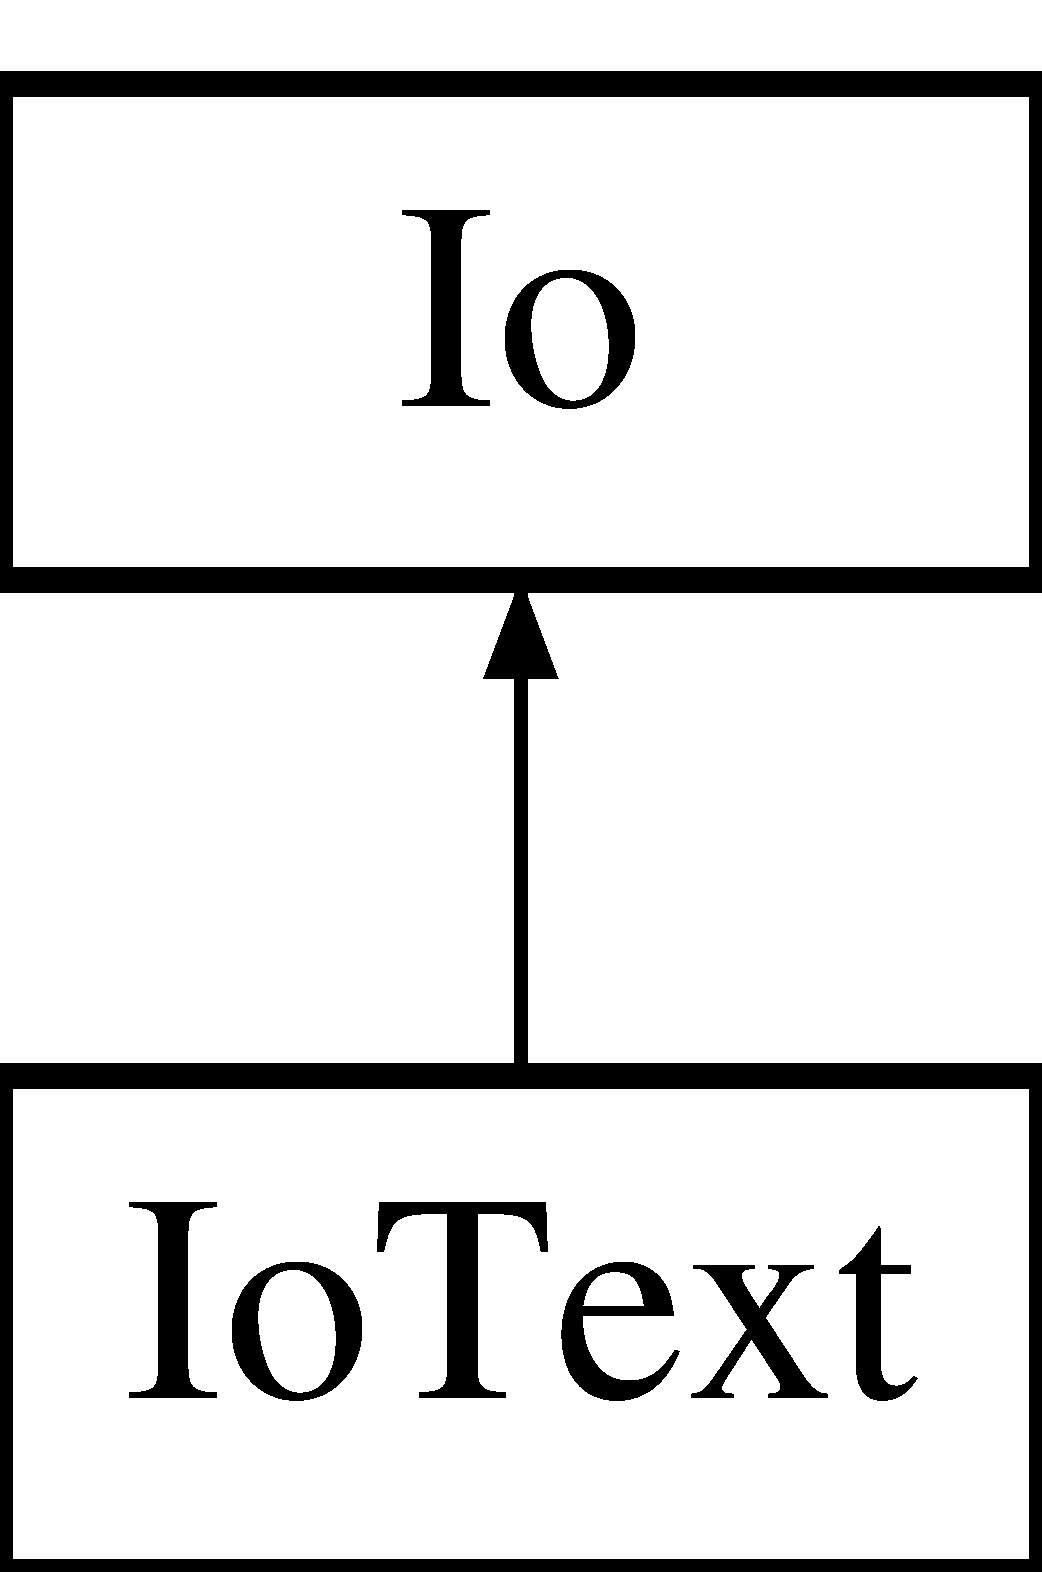
\includegraphics[height=2.000000cm]{structIoText}
\end{center}
\end{figure}
\subsection*{Public Member Functions}
\begin{DoxyCompactItemize}
\item 
\mbox{\hyperlink{structIoText_acbd0c221f311371d83bfa7588ca33ae7}{Io\+Text}} (const string io\+\_\+file)
\item 
int \mbox{\hyperlink{structIoText_a934af2596137889fa5c1327ad9deb6eb}{read\+\_\+length}} (const string fname, long \&length) const
\item 
int \mbox{\hyperlink{structIoText_aeea2eefd12d47f25389e9d6796326188}{read\+\_\+width}} (const string fname, long \&width) const
\item 
int \mbox{\hyperlink{structIoText_a8b52bfc7c9345a5d540fe05a6008eba5}{read\+\_\+number}} (const string fname, long \&number) const
\item 
int \mbox{\hyperlink{structIoText_a61c9ac128bdfbf1030ce0c3a4e8a6df8}{write\+\_\+number}} (const string fname, const long \&number) const
\item 
int \mbox{\hyperlink{structIoText_a36c615a44412abd5f1eb1dae9cc658b5}{read\+\_\+number}} (const string fname, double \&number) const
\item 
int \mbox{\hyperlink{structIoText_a6961384e467dd7a633230f1b943eee9b}{write\+\_\+number}} (const string fname, const double \&number) const
\item 
int \mbox{\hyperlink{structIoText_a5db69325c5a31309d77144498a7530cd}{read\+\_\+word}} (const string fname, string \&word) const
\item 
int \mbox{\hyperlink{structIoText_a222b88fc1ad28ebc0d2ef93642594823}{write\+\_\+word}} (const string fname, const string \&word) const
\item 
int \mbox{\hyperlink{structIoText_a2e8bfb3de876ac45dd0bf80081f75f52}{read\+\_\+list}} (const string fname, Long1 \&list) const
\item 
int \mbox{\hyperlink{structIoText_a8811cf2fddceef21dac759feb2d606f7}{write\+\_\+list}} (const string fname, const Long1 \&list) const
\item 
int \mbox{\hyperlink{structIoText_a86c3907450b95c9bbc895f5e66c266ab}{read\+\_\+list}} (const string fname, Double1 \&list) const
\item 
int \mbox{\hyperlink{structIoText_a7b2dbef1eb611ee8812b665f2499a3f9}{write\+\_\+list}} (const string fname, const Double1 \&list) const
\item 
int \mbox{\hyperlink{structIoText_a2aa750808cede99dd912cb93ca522995}{read\+\_\+list}} (const string fname, String1 \&list) const
\item 
int \mbox{\hyperlink{structIoText_a00ff0f739766d736557f44aa4ac0f34f}{write\+\_\+list}} (const string fname, const String1 \&list) const
\item 
int \mbox{\hyperlink{structIoText_a578827ab1f2e3c02dcd35d7d554f04b3}{read\+\_\+array}} (const string fname, Long2 \&array) const
\item 
int \mbox{\hyperlink{structIoText_a92319cdc25084941070cfc9d4fbd2feb}{write\+\_\+array}} (const string fname, const Long2 \&array) const
\item 
int \mbox{\hyperlink{structIoText_a732c8d4dfdeb8c1a8f139427ce4cef20}{read\+\_\+array}} (const string fname, Double2 \&array) const
\item 
int \mbox{\hyperlink{structIoText_a6382d40981a90b3fb3fe8e33bbc3f50e}{write\+\_\+array}} (const string fname, const Double2 \&array) const
\item 
int \mbox{\hyperlink{structIoText_a6984cd43f514a75a120cb63ee1b270dc}{read\+\_\+3\+\_\+vector}} (const string fname, Double1 \&x, Double1 \&y, Double1 \&z) const
\item 
int \mbox{\hyperlink{structIoText_a82af8045d5527d879c12dee52c9c2071}{write\+\_\+3\+\_\+vector}} (const string fname, const Double1 \&x, const Double1 \&y, const Double1 \&z) const
\end{DoxyCompactItemize}
\subsection*{Additional Inherited Members}


\subsection{Detailed Description}
\mbox{\hyperlink{structIoText}{Io\+Text}}\+: io specified by text files. 

\subsection{Constructor \& Destructor Documentation}
\mbox{\Hypertarget{structIoText_acbd0c221f311371d83bfa7588ca33ae7}\label{structIoText_acbd0c221f311371d83bfa7588ca33ae7}} 
\index{Io\+Text@{Io\+Text}!Io\+Text@{Io\+Text}}
\index{Io\+Text@{Io\+Text}!Io\+Text@{Io\+Text}}
\subsubsection{\texorpdfstring{Io\+Text()}{IoText()}}
{\footnotesize\ttfamily Io\+Text\+::\+Io\+Text (\begin{DoxyParamCaption}\item[{const string}]{io\+\_\+file }\end{DoxyParamCaption})}

Constructor for \mbox{\hyperlink{structIoText}{Io\+Text}} 
\begin{DoxyParams}[1]{Parameters}
\mbox{\tt in}  & {\em io\+\_\+file} & file to read from and write to \\
\hline
\end{DoxyParams}


\subsection{Member Function Documentation}
\mbox{\Hypertarget{structIoText_a6984cd43f514a75a120cb63ee1b270dc}\label{structIoText_a6984cd43f514a75a120cb63ee1b270dc}} 
\index{Io\+Text@{Io\+Text}!read\+\_\+3\+\_\+vector@{read\+\_\+3\+\_\+vector}}
\index{read\+\_\+3\+\_\+vector@{read\+\_\+3\+\_\+vector}!Io\+Text@{Io\+Text}}
\subsubsection{\texorpdfstring{read\+\_\+3\+\_\+vector()}{read\_3\_vector()}}
{\footnotesize\ttfamily int Io\+Text\+::read\+\_\+3\+\_\+vector (\begin{DoxyParamCaption}\item[{const string}]{file\+\_\+name,  }\item[{Double1 \&}]{x,  }\item[{Double1 \&}]{y,  }\item[{Double1 \&}]{z }\end{DoxyParamCaption}) const\hspace{0.3cm}{\ttfamily [virtual]}}

read\+\_\+3\+\_\+vector\+: 
\begin{DoxyParams}[1]{Parameters}
\mbox{\tt in}  & {\em file\+\_\+name} & path to file containing the data \\
\hline
\mbox{\tt in}  & {\em x} & x component of the vector to be read \\
\hline
\mbox{\tt in}  & {\em y} & y component of the vector to be read \\
\hline
\mbox{\tt in}  & {\em z} & z component of the vector to be read \\
\hline
\end{DoxyParams}


Implements \mbox{\hyperlink{structIo}{Io}}.

\mbox{\Hypertarget{structIoText_a578827ab1f2e3c02dcd35d7d554f04b3}\label{structIoText_a578827ab1f2e3c02dcd35d7d554f04b3}} 
\index{Io\+Text@{Io\+Text}!read\+\_\+array@{read\+\_\+array}}
\index{read\+\_\+array@{read\+\_\+array}!Io\+Text@{Io\+Text}}
\subsubsection{\texorpdfstring{read\+\_\+array()}{read\_array()}\hspace{0.1cm}{\footnotesize\ttfamily [1/2]}}
{\footnotesize\ttfamily int Io\+Text\+::read\+\_\+array (\begin{DoxyParamCaption}\item[{const string}]{file\+\_\+name,  }\item[{Long2 \&}]{array }\end{DoxyParamCaption}) const\hspace{0.3cm}{\ttfamily [virtual]}}

read\+\_\+array\+: 
\begin{DoxyParams}[1]{Parameters}
\mbox{\tt in}  & {\em file\+\_\+name} & path to file containing the data \\
\hline
\mbox{\tt in}  & {\em list} & array to be filled \\
\hline
\end{DoxyParams}


Implements \mbox{\hyperlink{structIo}{Io}}.

\mbox{\Hypertarget{structIoText_a732c8d4dfdeb8c1a8f139427ce4cef20}\label{structIoText_a732c8d4dfdeb8c1a8f139427ce4cef20}} 
\index{Io\+Text@{Io\+Text}!read\+\_\+array@{read\+\_\+array}}
\index{read\+\_\+array@{read\+\_\+array}!Io\+Text@{Io\+Text}}
\subsubsection{\texorpdfstring{read\+\_\+array()}{read\_array()}\hspace{0.1cm}{\footnotesize\ttfamily [2/2]}}
{\footnotesize\ttfamily int Io\+Text\+::read\+\_\+array (\begin{DoxyParamCaption}\item[{const string}]{file\+\_\+name,  }\item[{Double2 \&}]{array }\end{DoxyParamCaption}) const\hspace{0.3cm}{\ttfamily [virtual]}}

read\+\_\+array\+: 
\begin{DoxyParams}[1]{Parameters}
\mbox{\tt in}  & {\em file\+\_\+name} & path to file containing the data \\
\hline
\mbox{\tt in}  & {\em list} & array to be filled \\
\hline
\end{DoxyParams}


Implements \mbox{\hyperlink{structIo}{Io}}.

\mbox{\Hypertarget{structIoText_a934af2596137889fa5c1327ad9deb6eb}\label{structIoText_a934af2596137889fa5c1327ad9deb6eb}} 
\index{Io\+Text@{Io\+Text}!read\+\_\+length@{read\+\_\+length}}
\index{read\+\_\+length@{read\+\_\+length}!Io\+Text@{Io\+Text}}
\subsubsection{\texorpdfstring{read\+\_\+length()}{read\_length()}}
{\footnotesize\ttfamily int Io\+Text\+::read\+\_\+length (\begin{DoxyParamCaption}\item[{const string}]{file\+\_\+name,  }\item[{long \&}]{length }\end{DoxyParamCaption}) const\hspace{0.3cm}{\ttfamily [virtual]}}

get\+\_\+length\+: 
\begin{DoxyParams}[1]{Parameters}
\mbox{\tt in}  & {\em file\+\_\+name} & path to file containing the data \\
\hline
\mbox{\tt out}  & {\em length} & length to be read \\
\hline
\end{DoxyParams}


Implements \mbox{\hyperlink{structIo}{Io}}.

\mbox{\Hypertarget{structIoText_a2e8bfb3de876ac45dd0bf80081f75f52}\label{structIoText_a2e8bfb3de876ac45dd0bf80081f75f52}} 
\index{Io\+Text@{Io\+Text}!read\+\_\+list@{read\+\_\+list}}
\index{read\+\_\+list@{read\+\_\+list}!Io\+Text@{Io\+Text}}
\subsubsection{\texorpdfstring{read\+\_\+list()}{read\_list()}\hspace{0.1cm}{\footnotesize\ttfamily [1/3]}}
{\footnotesize\ttfamily int Io\+Text\+::read\+\_\+list (\begin{DoxyParamCaption}\item[{const string}]{file\+\_\+name,  }\item[{Long1 \&}]{list }\end{DoxyParamCaption}) const\hspace{0.3cm}{\ttfamily [virtual]}}

read\+\_\+list\+: 
\begin{DoxyParams}[1]{Parameters}
\mbox{\tt in}  & {\em file\+\_\+name} & path to file containing the data \\
\hline
\mbox{\tt in}  & {\em list} & list to be filled \\
\hline
\end{DoxyParams}


Implements \mbox{\hyperlink{structIo}{Io}}.

\mbox{\Hypertarget{structIoText_a86c3907450b95c9bbc895f5e66c266ab}\label{structIoText_a86c3907450b95c9bbc895f5e66c266ab}} 
\index{Io\+Text@{Io\+Text}!read\+\_\+list@{read\+\_\+list}}
\index{read\+\_\+list@{read\+\_\+list}!Io\+Text@{Io\+Text}}
\subsubsection{\texorpdfstring{read\+\_\+list()}{read\_list()}\hspace{0.1cm}{\footnotesize\ttfamily [2/3]}}
{\footnotesize\ttfamily int Io\+Text\+::read\+\_\+list (\begin{DoxyParamCaption}\item[{const string}]{file\+\_\+name,  }\item[{Double1 \&}]{list }\end{DoxyParamCaption}) const\hspace{0.3cm}{\ttfamily [virtual]}}

read\+\_\+list\+: 
\begin{DoxyParams}[1]{Parameters}
\mbox{\tt in}  & {\em file\+\_\+name} & path to file containing the data \\
\hline
\mbox{\tt in}  & {\em list} & list to be filled \\
\hline
\end{DoxyParams}


Implements \mbox{\hyperlink{structIo}{Io}}.

\mbox{\Hypertarget{structIoText_a2aa750808cede99dd912cb93ca522995}\label{structIoText_a2aa750808cede99dd912cb93ca522995}} 
\index{Io\+Text@{Io\+Text}!read\+\_\+list@{read\+\_\+list}}
\index{read\+\_\+list@{read\+\_\+list}!Io\+Text@{Io\+Text}}
\subsubsection{\texorpdfstring{read\+\_\+list()}{read\_list()}\hspace{0.1cm}{\footnotesize\ttfamily [3/3]}}
{\footnotesize\ttfamily int Io\+Text\+::read\+\_\+list (\begin{DoxyParamCaption}\item[{const string}]{file\+\_\+name,  }\item[{String1 \&}]{list }\end{DoxyParamCaption}) const\hspace{0.3cm}{\ttfamily [virtual]}}

read\+\_\+list\+: 
\begin{DoxyParams}[1]{Parameters}
\mbox{\tt in}  & {\em file\+\_\+name} & path to file containing the data \\
\hline
\mbox{\tt in}  & {\em list} & list to be filled \\
\hline
\end{DoxyParams}


Implements \mbox{\hyperlink{structIo}{Io}}.

\mbox{\Hypertarget{structIoText_a8b52bfc7c9345a5d540fe05a6008eba5}\label{structIoText_a8b52bfc7c9345a5d540fe05a6008eba5}} 
\index{Io\+Text@{Io\+Text}!read\+\_\+number@{read\+\_\+number}}
\index{read\+\_\+number@{read\+\_\+number}!Io\+Text@{Io\+Text}}
\subsubsection{\texorpdfstring{read\+\_\+number()}{read\_number()}\hspace{0.1cm}{\footnotesize\ttfamily [1/2]}}
{\footnotesize\ttfamily int Io\+Text\+::read\+\_\+number (\begin{DoxyParamCaption}\item[{const string}]{file\+\_\+name,  }\item[{long \&}]{number }\end{DoxyParamCaption}) const\hspace{0.3cm}{\ttfamily [virtual]}}

read\+\_\+number\+: 
\begin{DoxyParams}[1]{Parameters}
\mbox{\tt in}  & {\em file\+\_\+name} & file containing the number \\
\hline
\mbox{\tt out}  & {\em number} & number to be read \\
\hline
\end{DoxyParams}


Implements \mbox{\hyperlink{structIo}{Io}}.

\mbox{\Hypertarget{structIoText_a36c615a44412abd5f1eb1dae9cc658b5}\label{structIoText_a36c615a44412abd5f1eb1dae9cc658b5}} 
\index{Io\+Text@{Io\+Text}!read\+\_\+number@{read\+\_\+number}}
\index{read\+\_\+number@{read\+\_\+number}!Io\+Text@{Io\+Text}}
\subsubsection{\texorpdfstring{read\+\_\+number()}{read\_number()}\hspace{0.1cm}{\footnotesize\ttfamily [2/2]}}
{\footnotesize\ttfamily int Io\+Text\+::read\+\_\+number (\begin{DoxyParamCaption}\item[{const string}]{file\+\_\+name,  }\item[{double \&}]{number }\end{DoxyParamCaption}) const\hspace{0.3cm}{\ttfamily [virtual]}}

read\+\_\+number\+: 
\begin{DoxyParams}[1]{Parameters}
\mbox{\tt in}  & {\em file\+\_\+name} & file containing the number \\
\hline
\mbox{\tt out}  & {\em number} & number to be read \\
\hline
\end{DoxyParams}


Implements \mbox{\hyperlink{structIo}{Io}}.

\mbox{\Hypertarget{structIoText_aeea2eefd12d47f25389e9d6796326188}\label{structIoText_aeea2eefd12d47f25389e9d6796326188}} 
\index{Io\+Text@{Io\+Text}!read\+\_\+width@{read\+\_\+width}}
\index{read\+\_\+width@{read\+\_\+width}!Io\+Text@{Io\+Text}}
\subsubsection{\texorpdfstring{read\+\_\+width()}{read\_width()}}
{\footnotesize\ttfamily int Io\+Text\+::read\+\_\+width (\begin{DoxyParamCaption}\item[{const string}]{file\+\_\+name,  }\item[{long \&}]{width }\end{DoxyParamCaption}) const\hspace{0.3cm}{\ttfamily [virtual]}}

get\+\_\+length\+: 
\begin{DoxyParams}[1]{Parameters}
\mbox{\tt in}  & {\em file\+\_\+name} & path to file containing the data \\
\hline
\mbox{\tt out}  & {\em length} & length to be read \\
\hline
\end{DoxyParams}


Implements \mbox{\hyperlink{structIo}{Io}}.

\mbox{\Hypertarget{structIoText_a5db69325c5a31309d77144498a7530cd}\label{structIoText_a5db69325c5a31309d77144498a7530cd}} 
\index{Io\+Text@{Io\+Text}!read\+\_\+word@{read\+\_\+word}}
\index{read\+\_\+word@{read\+\_\+word}!Io\+Text@{Io\+Text}}
\subsubsection{\texorpdfstring{read\+\_\+word()}{read\_word()}}
{\footnotesize\ttfamily int Io\+Text\+::read\+\_\+word (\begin{DoxyParamCaption}\item[{const string}]{file\+\_\+name,  }\item[{string \&}]{word }\end{DoxyParamCaption}) const\hspace{0.3cm}{\ttfamily [virtual]}}

read\+\_\+word\+: 
\begin{DoxyParams}[1]{Parameters}
\mbox{\tt in}  & {\em file\+\_\+name} & file containing the number \\
\hline
\end{DoxyParams}


Implements \mbox{\hyperlink{structIo}{Io}}.

\mbox{\Hypertarget{structIoText_a82af8045d5527d879c12dee52c9c2071}\label{structIoText_a82af8045d5527d879c12dee52c9c2071}} 
\index{Io\+Text@{Io\+Text}!write\+\_\+3\+\_\+vector@{write\+\_\+3\+\_\+vector}}
\index{write\+\_\+3\+\_\+vector@{write\+\_\+3\+\_\+vector}!Io\+Text@{Io\+Text}}
\subsubsection{\texorpdfstring{write\+\_\+3\+\_\+vector()}{write\_3\_vector()}}
{\footnotesize\ttfamily int Io\+Text\+::write\+\_\+3\+\_\+vector (\begin{DoxyParamCaption}\item[{const string}]{file\+\_\+name,  }\item[{const Double1 \&}]{x,  }\item[{const Double1 \&}]{y,  }\item[{const Double1 \&}]{z }\end{DoxyParamCaption}) const\hspace{0.3cm}{\ttfamily [virtual]}}

write\+\_\+3\+\_\+vector\+: 
\begin{DoxyParams}[1]{Parameters}
\mbox{\tt in}  & {\em file\+\_\+name} & path to file containing the data \\
\hline
\mbox{\tt in}  & {\em x} & x component of the vector to be written \\
\hline
\mbox{\tt in}  & {\em y} & y component of the vector to be written \\
\hline
\mbox{\tt in}  & {\em z} & z component of the vector to be written \\
\hline
\end{DoxyParams}


Implements \mbox{\hyperlink{structIo}{Io}}.

\mbox{\Hypertarget{structIoText_a92319cdc25084941070cfc9d4fbd2feb}\label{structIoText_a92319cdc25084941070cfc9d4fbd2feb}} 
\index{Io\+Text@{Io\+Text}!write\+\_\+array@{write\+\_\+array}}
\index{write\+\_\+array@{write\+\_\+array}!Io\+Text@{Io\+Text}}
\subsubsection{\texorpdfstring{write\+\_\+array()}{write\_array()}\hspace{0.1cm}{\footnotesize\ttfamily [1/2]}}
{\footnotesize\ttfamily int Io\+Text\+::write\+\_\+array (\begin{DoxyParamCaption}\item[{const string}]{file\+\_\+name,  }\item[{const Long2 \&}]{array }\end{DoxyParamCaption}) const\hspace{0.3cm}{\ttfamily [virtual]}}

write\+\_\+array\+: 
\begin{DoxyParams}[1]{Parameters}
\mbox{\tt in}  & {\em file\+\_\+name} & path to file containing the data \\
\hline
\mbox{\tt in}  & {\em list} & array to be written \\
\hline
\end{DoxyParams}


Implements \mbox{\hyperlink{structIo}{Io}}.

\mbox{\Hypertarget{structIoText_a6382d40981a90b3fb3fe8e33bbc3f50e}\label{structIoText_a6382d40981a90b3fb3fe8e33bbc3f50e}} 
\index{Io\+Text@{Io\+Text}!write\+\_\+array@{write\+\_\+array}}
\index{write\+\_\+array@{write\+\_\+array}!Io\+Text@{Io\+Text}}
\subsubsection{\texorpdfstring{write\+\_\+array()}{write\_array()}\hspace{0.1cm}{\footnotesize\ttfamily [2/2]}}
{\footnotesize\ttfamily int Io\+Text\+::write\+\_\+array (\begin{DoxyParamCaption}\item[{const string}]{file\+\_\+name,  }\item[{const Double2 \&}]{array }\end{DoxyParamCaption}) const\hspace{0.3cm}{\ttfamily [virtual]}}

write\+\_\+array\+: 
\begin{DoxyParams}[1]{Parameters}
\mbox{\tt in}  & {\em file\+\_\+name} & path to file containing the data \\
\hline
\mbox{\tt in}  & {\em list} & array to be written \\
\hline
\end{DoxyParams}


Implements \mbox{\hyperlink{structIo}{Io}}.

\mbox{\Hypertarget{structIoText_a8811cf2fddceef21dac759feb2d606f7}\label{structIoText_a8811cf2fddceef21dac759feb2d606f7}} 
\index{Io\+Text@{Io\+Text}!write\+\_\+list@{write\+\_\+list}}
\index{write\+\_\+list@{write\+\_\+list}!Io\+Text@{Io\+Text}}
\subsubsection{\texorpdfstring{write\+\_\+list()}{write\_list()}\hspace{0.1cm}{\footnotesize\ttfamily [1/3]}}
{\footnotesize\ttfamily int Io\+Text\+::write\+\_\+list (\begin{DoxyParamCaption}\item[{const string}]{file\+\_\+name,  }\item[{const Long1 \&}]{list }\end{DoxyParamCaption}) const\hspace{0.3cm}{\ttfamily [virtual]}}

write\+\_\+list\+: 
\begin{DoxyParams}[1]{Parameters}
\mbox{\tt in}  & {\em file\+\_\+name} & path to file containing the data \\
\hline
\mbox{\tt in}  & {\em list} & list to be written \\
\hline
\end{DoxyParams}


Implements \mbox{\hyperlink{structIo}{Io}}.

\mbox{\Hypertarget{structIoText_a7b2dbef1eb611ee8812b665f2499a3f9}\label{structIoText_a7b2dbef1eb611ee8812b665f2499a3f9}} 
\index{Io\+Text@{Io\+Text}!write\+\_\+list@{write\+\_\+list}}
\index{write\+\_\+list@{write\+\_\+list}!Io\+Text@{Io\+Text}}
\subsubsection{\texorpdfstring{write\+\_\+list()}{write\_list()}\hspace{0.1cm}{\footnotesize\ttfamily [2/3]}}
{\footnotesize\ttfamily int Io\+Text\+::write\+\_\+list (\begin{DoxyParamCaption}\item[{const string}]{file\+\_\+name,  }\item[{const Double1 \&}]{list }\end{DoxyParamCaption}) const\hspace{0.3cm}{\ttfamily [virtual]}}

write\+\_\+list\+: 
\begin{DoxyParams}[1]{Parameters}
\mbox{\tt in}  & {\em file\+\_\+name} & path to file containing the data \\
\hline
\mbox{\tt in}  & {\em list} & list to be written \\
\hline
\end{DoxyParams}


Implements \mbox{\hyperlink{structIo}{Io}}.

\mbox{\Hypertarget{structIoText_a00ff0f739766d736557f44aa4ac0f34f}\label{structIoText_a00ff0f739766d736557f44aa4ac0f34f}} 
\index{Io\+Text@{Io\+Text}!write\+\_\+list@{write\+\_\+list}}
\index{write\+\_\+list@{write\+\_\+list}!Io\+Text@{Io\+Text}}
\subsubsection{\texorpdfstring{write\+\_\+list()}{write\_list()}\hspace{0.1cm}{\footnotesize\ttfamily [3/3]}}
{\footnotesize\ttfamily int Io\+Text\+::write\+\_\+list (\begin{DoxyParamCaption}\item[{const string}]{file\+\_\+name,  }\item[{const String1 \&}]{list }\end{DoxyParamCaption}) const\hspace{0.3cm}{\ttfamily [virtual]}}

write\+\_\+list\+: 
\begin{DoxyParams}[1]{Parameters}
\mbox{\tt in}  & {\em file\+\_\+name} & path to file containing the data \\
\hline
\mbox{\tt in}  & {\em list} & list to be written \\
\hline
\end{DoxyParams}


Implements \mbox{\hyperlink{structIo}{Io}}.

\mbox{\Hypertarget{structIoText_a61c9ac128bdfbf1030ce0c3a4e8a6df8}\label{structIoText_a61c9ac128bdfbf1030ce0c3a4e8a6df8}} 
\index{Io\+Text@{Io\+Text}!write\+\_\+number@{write\+\_\+number}}
\index{write\+\_\+number@{write\+\_\+number}!Io\+Text@{Io\+Text}}
\subsubsection{\texorpdfstring{write\+\_\+number()}{write\_number()}\hspace{0.1cm}{\footnotesize\ttfamily [1/2]}}
{\footnotesize\ttfamily int Io\+Text\+::write\+\_\+number (\begin{DoxyParamCaption}\item[{const string}]{file\+\_\+name,  }\item[{const long \&}]{number }\end{DoxyParamCaption}) const\hspace{0.3cm}{\ttfamily [virtual]}}

write\+\_\+number\+: 
\begin{DoxyParams}[1]{Parameters}
\mbox{\tt in}  & {\em file\+\_\+name} & file containing the number \\
\hline
\mbox{\tt out}  & {\em number} & number to be written \\
\hline
\end{DoxyParams}


Implements \mbox{\hyperlink{structIo}{Io}}.

\mbox{\Hypertarget{structIoText_a6961384e467dd7a633230f1b943eee9b}\label{structIoText_a6961384e467dd7a633230f1b943eee9b}} 
\index{Io\+Text@{Io\+Text}!write\+\_\+number@{write\+\_\+number}}
\index{write\+\_\+number@{write\+\_\+number}!Io\+Text@{Io\+Text}}
\subsubsection{\texorpdfstring{write\+\_\+number()}{write\_number()}\hspace{0.1cm}{\footnotesize\ttfamily [2/2]}}
{\footnotesize\ttfamily int Io\+Text\+::write\+\_\+number (\begin{DoxyParamCaption}\item[{const string}]{file\+\_\+name,  }\item[{const double \&}]{number }\end{DoxyParamCaption}) const\hspace{0.3cm}{\ttfamily [virtual]}}

write\+\_\+number\+: 
\begin{DoxyParams}[1]{Parameters}
\mbox{\tt in}  & {\em file\+\_\+name} & file containing the number \\
\hline
\mbox{\tt out}  & {\em number} & number to be written \\
\hline
\end{DoxyParams}


Implements \mbox{\hyperlink{structIo}{Io}}.

\mbox{\Hypertarget{structIoText_a222b88fc1ad28ebc0d2ef93642594823}\label{structIoText_a222b88fc1ad28ebc0d2ef93642594823}} 
\index{Io\+Text@{Io\+Text}!write\+\_\+word@{write\+\_\+word}}
\index{write\+\_\+word@{write\+\_\+word}!Io\+Text@{Io\+Text}}
\subsubsection{\texorpdfstring{write\+\_\+word()}{write\_word()}}
{\footnotesize\ttfamily int Io\+Text\+::write\+\_\+word (\begin{DoxyParamCaption}\item[{const string}]{file\+\_\+name,  }\item[{const string \&}]{word }\end{DoxyParamCaption}) const\hspace{0.3cm}{\ttfamily [virtual]}}

write\+\_\+word\+: 
\begin{DoxyParams}[1]{Parameters}
\mbox{\tt in}  & {\em file\+\_\+name} & file containing the number \\
\hline
\end{DoxyParams}


Implements \mbox{\hyperlink{structIo}{Io}}.



The documentation for this struct was generated from the following files\+:\begin{DoxyCompactItemize}
\item 
/home/frederik/\+Dropbox/\+Astro/\+Magritte/src/\+Io/cpp/io\+\_\+cpp\+\_\+text.\+hpp\item 
/home/frederik/\+Dropbox/\+Astro/\+Magritte/src/\+Io/cpp/io\+\_\+cpp\+\_\+text.\+cpp\end{DoxyCompactItemize}

\hypertarget{structLambda}{}\section{Lambda Struct Reference}
\label{structLambda}\index{Lambda@{Lambda}}


\mbox{\hyperlink{structLambda}{Lambda}}\+: data structure for the \mbox{\hyperlink{structLambda}{Lambda}} oprator.  




{\ttfamily \#include $<$lambda.\+hpp$>$}

\subsection*{Public Member Functions}
\begin{DoxyCompactItemize}
\item 
\mbox{\Hypertarget{structLambda_a501c4088dfc430615ccb7aa7f55de187}\label{structLambda_a501c4088dfc430615ccb7aa7f55de187}} 
void {\bfseries add\+\_\+entry} (const double Ls, const long nr)
\end{DoxyCompactItemize}
\subsection*{Public Attributes}
\begin{DoxyCompactItemize}
\item 
\mbox{\Hypertarget{structLambda_a037c9579f00f5477ed1c73cd3866a11c}\label{structLambda_a037c9579f00f5477ed1c73cd3866a11c}} 
Double1 {\bfseries Ls}
\item 
\mbox{\Hypertarget{structLambda_a635eaeecc104cb55a907a75c4edad89a}\label{structLambda_a635eaeecc104cb55a907a75c4edad89a}} 
Long1 {\bfseries nr}
\end{DoxyCompactItemize}


\subsection{Detailed Description}
\mbox{\hyperlink{structLambda}{Lambda}}\+: data structure for the \mbox{\hyperlink{structLambda}{Lambda}} oprator. 

The documentation for this struct was generated from the following file\+:\begin{DoxyCompactItemize}
\item 
/home/frederik/\+Dropbox/\+Astro/\+Magritte/src/\+Model/\+Lines/\+Line\+Producing\+Species/\+Lambda/lambda.\+hpp\end{DoxyCompactItemize}

\hypertarget{structLinedata}{}\section{Linedata Struct Reference}
\label{structLinedata}\index{Linedata@{Linedata}}
\subsection*{Public Member Functions}
\begin{DoxyCompactItemize}
\item 
int \mbox{\hyperlink{structLinedata_af4cb38e89e417f7016608b7084223364}{read}} (const \mbox{\hyperlink{structIo}{Io}} \&io, const int l)
\item 
int \mbox{\hyperlink{structLinedata_a790d9790b8a7ac3c613bd4c27155135b}{write}} (const \mbox{\hyperlink{structIo}{Io}} \&io, const int l) const
\end{DoxyCompactItemize}
\subsection*{Public Attributes}
\begin{DoxyCompactItemize}
\item 
\mbox{\Hypertarget{structLinedata_a31cad37c5cab2d17996b8efce5308e06}\label{structLinedata_a31cad37c5cab2d17996b8efce5308e06}} 
long \mbox{\hyperlink{structLinedata_a31cad37c5cab2d17996b8efce5308e06}{num}}
\begin{DoxyCompactList}\small\item\em number of line producing species \end{DoxyCompactList}\item 
\mbox{\Hypertarget{structLinedata_ab6519202beb7c464418295a9b65e044c}\label{structLinedata_ab6519202beb7c464418295a9b65e044c}} 
string \mbox{\hyperlink{structLinedata_ab6519202beb7c464418295a9b65e044c}{sym}}
\begin{DoxyCompactList}\small\item\em symbol of line producing species \end{DoxyCompactList}\item 
\mbox{\Hypertarget{structLinedata_adbb1b0fe9d8d409c26d764a3a4a8985b}\label{structLinedata_adbb1b0fe9d8d409c26d764a3a4a8985b}} 
double \mbox{\hyperlink{structLinedata_adbb1b0fe9d8d409c26d764a3a4a8985b}{inverse\+\_\+mass}}
\begin{DoxyCompactList}\small\item\em 1/mass of line producing species \end{DoxyCompactList}\item 
\mbox{\Hypertarget{structLinedata_a2475c8cd835885bf01071f6d11c41e86}\label{structLinedata_a2475c8cd835885bf01071f6d11c41e86}} 
long \mbox{\hyperlink{structLinedata_a2475c8cd835885bf01071f6d11c41e86}{nlev}}
\begin{DoxyCompactList}\small\item\em number of levels \end{DoxyCompactList}\item 
\mbox{\Hypertarget{structLinedata_a9b057d75ef956bbec3d0efe352836382}\label{structLinedata_a9b057d75ef956bbec3d0efe352836382}} 
long \mbox{\hyperlink{structLinedata_a9b057d75ef956bbec3d0efe352836382}{nrad}}
\begin{DoxyCompactList}\small\item\em number of radiative transitions \end{DoxyCompactList}\item 
\mbox{\Hypertarget{structLinedata_a38f48360b128abcb7fb6467fa7594591}\label{structLinedata_a38f48360b128abcb7fb6467fa7594591}} 
Long1 \mbox{\hyperlink{structLinedata_a38f48360b128abcb7fb6467fa7594591}{irad}}
\begin{DoxyCompactList}\small\item\em level index of radiative transition \end{DoxyCompactList}\item 
\mbox{\Hypertarget{structLinedata_af45902e70adadfa03f63449f30f89ea4}\label{structLinedata_af45902e70adadfa03f63449f30f89ea4}} 
Long1 \mbox{\hyperlink{structLinedata_af45902e70adadfa03f63449f30f89ea4}{jrad}}
\begin{DoxyCompactList}\small\item\em level index of radiative transition \end{DoxyCompactList}\item 
\mbox{\Hypertarget{structLinedata_a7e997b9f5dfcc8de98c490da07eb9c99}\label{structLinedata_a7e997b9f5dfcc8de98c490da07eb9c99}} 
Double1 \mbox{\hyperlink{structLinedata_a7e997b9f5dfcc8de98c490da07eb9c99}{energy}}
\begin{DoxyCompactList}\small\item\em energy of level \end{DoxyCompactList}\item 
\mbox{\Hypertarget{structLinedata_a7a49ab1a4d94bee039b6ae6b3e2b157e}\label{structLinedata_a7a49ab1a4d94bee039b6ae6b3e2b157e}} 
Double1 \mbox{\hyperlink{structLinedata_a7a49ab1a4d94bee039b6ae6b3e2b157e}{weight}}
\begin{DoxyCompactList}\small\item\em weight of level (statistical) \end{DoxyCompactList}\item 
\mbox{\Hypertarget{structLinedata_ae900dd3f78aa49277a9c26787241607b}\label{structLinedata_ae900dd3f78aa49277a9c26787241607b}} 
Double1 \mbox{\hyperlink{structLinedata_ae900dd3f78aa49277a9c26787241607b}{frequency}}
\begin{DoxyCompactList}\small\item\em frequency corresponding to each transition \end{DoxyCompactList}\item 
\mbox{\Hypertarget{structLinedata_a3f0e414cf016f18f9a7a86ffbb2207b7}\label{structLinedata_a3f0e414cf016f18f9a7a86ffbb2207b7}} 
Double1 \mbox{\hyperlink{structLinedata_a3f0e414cf016f18f9a7a86ffbb2207b7}{A}}
\begin{DoxyCompactList}\small\item\em Einstein A (spontaneous emission) \end{DoxyCompactList}\item 
\mbox{\Hypertarget{structLinedata_a2a0a095bd74c0b4333307c8f73f74662}\label{structLinedata_a2a0a095bd74c0b4333307c8f73f74662}} 
Double1 \mbox{\hyperlink{structLinedata_a2a0a095bd74c0b4333307c8f73f74662}{Ba}}
\begin{DoxyCompactList}\small\item\em Einstsin Ba (absorption) \end{DoxyCompactList}\item 
\mbox{\Hypertarget{structLinedata_ab97d931f484320c16c7d9fa8bf67bde3}\label{structLinedata_ab97d931f484320c16c7d9fa8bf67bde3}} 
Double1 \mbox{\hyperlink{structLinedata_ab97d931f484320c16c7d9fa8bf67bde3}{Bs}}
\begin{DoxyCompactList}\small\item\em Einstein Bs (stimulated emission) \end{DoxyCompactList}\item 
\mbox{\Hypertarget{structLinedata_a82744cd6d4c56bb2b4b9d53c3f574560}\label{structLinedata_a82744cd6d4c56bb2b4b9d53c3f574560}} 
long \mbox{\hyperlink{structLinedata_a82744cd6d4c56bb2b4b9d53c3f574560}{ncolpar}}
\begin{DoxyCompactList}\small\item\em number of collision partners \end{DoxyCompactList}\item 
\mbox{\Hypertarget{structLinedata_a89bee23ead1d6b1f80106c39d802e5d2}\label{structLinedata_a89bee23ead1d6b1f80106c39d802e5d2}} 
std\+::vector$<$ \mbox{\hyperlink{structCollisionPartner}{Collision\+Partner}} $>$ \mbox{\hyperlink{structLinedata_a89bee23ead1d6b1f80106c39d802e5d2}{colpar}}
\begin{DoxyCompactList}\small\item\em Vector containing collision partner data. \end{DoxyCompactList}\item 
\mbox{\Hypertarget{structLinedata_a492753995a2c3bf15b6705764746f199}\label{structLinedata_a492753995a2c3bf15b6705764746f199}} 
long {\bfseries ncol\+\_\+tot}
\end{DoxyCompactItemize}


\subsection{Member Function Documentation}
\mbox{\Hypertarget{structLinedata_af4cb38e89e417f7016608b7084223364}\label{structLinedata_af4cb38e89e417f7016608b7084223364}} 
\index{Linedata@{Linedata}!read@{read}}
\index{read@{read}!Linedata@{Linedata}}
\subsubsection{\texorpdfstring{read()}{read()}}
{\footnotesize\ttfamily int Linedata\+::read (\begin{DoxyParamCaption}\item[{const \mbox{\hyperlink{structIo}{Io}} \&}]{io,  }\item[{const int}]{l }\end{DoxyParamCaption})}

read\+: read in line data 
\begin{DoxyParams}[1]{Parameters}
\mbox{\tt in}  & {\em io} & io object \\
\hline
\mbox{\tt in}  & {\em l} & nr of line producing species \\
\hline
\end{DoxyParams}
\mbox{\Hypertarget{structLinedata_a790d9790b8a7ac3c613bd4c27155135b}\label{structLinedata_a790d9790b8a7ac3c613bd4c27155135b}} 
\index{Linedata@{Linedata}!write@{write}}
\index{write@{write}!Linedata@{Linedata}}
\subsubsection{\texorpdfstring{write()}{write()}}
{\footnotesize\ttfamily int Linedata\+::write (\begin{DoxyParamCaption}\item[{const \mbox{\hyperlink{structIo}{Io}} \&}]{io,  }\item[{const int}]{l }\end{DoxyParamCaption}) const}

write\+: write out data structure 
\begin{DoxyParams}[1]{Parameters}
\mbox{\tt in}  & {\em io} & io object \\
\hline
\mbox{\tt in}  & {\em l} & nr of line producing species \\
\hline
\end{DoxyParams}


The documentation for this struct was generated from the following files\+:\begin{DoxyCompactItemize}
\item 
/home/frederik/\+Dropbox/\+Astro/\+Magritte/src/\+Model/\+Lines/\+Line\+Producing\+Species/\+Linedata/linedata.\+hpp\item 
/home/frederik/\+Dropbox/\+Astro/\+Magritte/src/\+Model/\+Lines/\+Line\+Producing\+Species/\+Linedata/linedata.\+cpp\end{DoxyCompactItemize}

\hypertarget{structLineProducingSpecies}{}\section{Line\+Producing\+Species Struct Reference}
\label{structLineProducingSpecies}\index{Line\+Producing\+Species@{Line\+Producing\+Species}}
\subsection*{Public Member Functions}
\begin{DoxyCompactItemize}
\item 
int \mbox{\hyperlink{structLineProducingSpecies_a682268d3085f8ca3d24b278df757f141}{read}} (const \mbox{\hyperlink{structIo}{Io}} \&io, const long l, \mbox{\hyperlink{classParameters}{Parameters}} \&parameters)
\item 
int \mbox{\hyperlink{structLineProducingSpecies_a9152eaa80ee71288e3bdc05e749939b6}{write}} (const \mbox{\hyperlink{structIo}{Io}} \&io, const long l) const
\item 
int \mbox{\hyperlink{structLineProducingSpecies_ab6062b14b7d076bffedb96b3d61fc1d4}{write\+\_\+populations}} (const \mbox{\hyperlink{structIo}{Io}} \&io, const long l, const string tag) const
\item 
\mbox{\Hypertarget{structLineProducingSpecies_a1ef68cebbf968f57e3190f385cfda6e6}\label{structLineProducingSpecies_a1ef68cebbf968f57e3190f385cfda6e6}} 
long {\bfseries index} (const long p, const long i) const
\item 
\mbox{\Hypertarget{structLineProducingSpecies_a17b5c3f00749cdcff0f575fcd99fd92a}\label{structLineProducingSpecies_a17b5c3f00749cdcff0f575fcd99fd92a}} 
double {\bfseries get\+\_\+emissivity} (const long p, const long k) const
\item 
\mbox{\Hypertarget{structLineProducingSpecies_a83d52693fc6a050402fe93ccdcd47500}\label{structLineProducingSpecies_a83d52693fc6a050402fe93ccdcd47500}} 
double {\bfseries get\+\_\+opacity} (const long p, const long k) const
\item 
\mbox{\Hypertarget{structLineProducingSpecies_a7b7415df082a8dc660fde417ece3aced}\label{structLineProducingSpecies_a7b7415df082a8dc660fde417ece3aced}} 
void {\bfseries check\+\_\+for\+\_\+convergence} (const double pop\+\_\+prec)
\item 
\mbox{\Hypertarget{structLineProducingSpecies_ae55c10a0b41b332d78c640bd72c169bc}\label{structLineProducingSpecies_ae55c10a0b41b332d78c640bd72c169bc}} 
void {\bfseries update\+\_\+using\+\_\+\+L\+TE} (const Double2 \&abundance, const Double1 \&temperature)
\item 
\mbox{\Hypertarget{structLineProducingSpecies_a95c95f687306608a8aff6e26ae5bd848}\label{structLineProducingSpecies_a95c95f687306608a8aff6e26ae5bd848}} 
void {\bfseries update\+\_\+using\+\_\+statistical\+\_\+equilibrium} (const Double2 \&abundance, const Double1 \&temperature)
\item 
\mbox{\Hypertarget{structLineProducingSpecies_aea9a3fc9d735fa6b5238c44fd38296aa}\label{structLineProducingSpecies_aea9a3fc9d735fa6b5238c44fd38296aa}} 
void {\bfseries update\+\_\+using\+\_\+\+Ng\+\_\+acceleration} ()
\item 
\mbox{\Hypertarget{structLineProducingSpecies_a8400c3ec984ab4fc25174c39954342c9}\label{structLineProducingSpecies_a8400c3ec984ab4fc25174c39954342c9}} 
int \mbox{\hyperlink{structLineProducingSpecies_a8400c3ec984ab4fc25174c39954342c9}{initialize\+\_\+\+Lambda}} ()
\begin{DoxyCompactList}\small\item\em initialize\+\_\+\+Lambda\+: clear all entries of \mbox{\hyperlink{structLambda}{Lambda}} operator \end{DoxyCompactList}\item 
\mbox{\Hypertarget{structLineProducingSpecies_ade61c881ebf614736992e173f8c0cc3c}\label{structLineProducingSpecies_ade61c881ebf614736992e173f8c0cc3c}} 
int \mbox{\hyperlink{structLineProducingSpecies_ade61c881ebf614736992e173f8c0cc3c}{gather\+\_\+\+Lambda}} ()
\begin{DoxyCompactList}\small\item\em gather\+\_\+\+Lambda\+: gather \mbox{\hyperlink{structLambda}{Lambda}}\textquotesingle{}s from M\+PI distributed processes \end{DoxyCompactList}\end{DoxyCompactItemize}
\subsection*{Public Attributes}
\begin{DoxyCompactItemize}
\item 
\mbox{\Hypertarget{structLineProducingSpecies_af82c9246277856fe9a85fee5efc020a9}\label{structLineProducingSpecies_af82c9246277856fe9a85fee5efc020a9}} 
\mbox{\hyperlink{structLinedata}{Linedata}} \mbox{\hyperlink{structLineProducingSpecies_af82c9246277856fe9a85fee5efc020a9}{linedata}}
\begin{DoxyCompactList}\small\item\em data for line producing species \end{DoxyCompactList}\item 
\mbox{\Hypertarget{structLineProducingSpecies_a5ddef72c65be1892caa3260ff4c671fb}\label{structLineProducingSpecies_a5ddef72c65be1892caa3260ff4c671fb}} 
\mbox{\hyperlink{structQuadrature}{Quadrature}} \mbox{\hyperlink{structLineProducingSpecies_a5ddef72c65be1892caa3260ff4c671fb}{quadrature}}
\begin{DoxyCompactList}\small\item\em data for integral over line \end{DoxyCompactList}\item 
\mbox{\Hypertarget{structLineProducingSpecies_a476b6eff37715b47fcece3ea21bea8f9}\label{structLineProducingSpecies_a476b6eff37715b47fcece3ea21bea8f9}} 
std\+::vector$<$ std\+::vector$<$ \mbox{\hyperlink{structLambda}{Lambda}} $>$ $>$ {\bfseries lambda}
\item 
\mbox{\Hypertarget{structLineProducingSpecies_a633ab10bbe9df398e2ad92fe4dc082c0}\label{structLineProducingSpecies_a633ab10bbe9df398e2ad92fe4dc082c0}} 
Double2 {\bfseries Jeff}
\item 
\mbox{\Hypertarget{structLineProducingSpecies_a3de194bf4535cff2d431bf1e337c5df6}\label{structLineProducingSpecies_a3de194bf4535cff2d431bf1e337c5df6}} 
Double2 {\bfseries Jlin}
\item 
\mbox{\Hypertarget{structLineProducingSpecies_af3112742ce529751bcd6d370fbb25ec6}\label{structLineProducingSpecies_af3112742ce529751bcd6d370fbb25ec6}} 
Long3 \mbox{\hyperlink{structLineProducingSpecies_af3112742ce529751bcd6d370fbb25ec6}{nr\+\_\+line}}
\begin{DoxyCompactList}\small\item\em frequency number corresponing to line (p,k,z) \end{DoxyCompactList}\item 
\mbox{\Hypertarget{structLineProducingSpecies_a0c056f43cef52d62974c1ade2ad215b5}\label{structLineProducingSpecies_a0c056f43cef52d62974c1ade2ad215b5}} 
double \mbox{\hyperlink{structLineProducingSpecies_a0c056f43cef52d62974c1ade2ad215b5}{relative\+\_\+change\+\_\+mean}}
\begin{DoxyCompactList}\small\item\em mean relative change \end{DoxyCompactList}\item 
\mbox{\Hypertarget{structLineProducingSpecies_a884352a22da6800b6e43638855bb4a89}\label{structLineProducingSpecies_a884352a22da6800b6e43638855bb4a89}} 
double \mbox{\hyperlink{structLineProducingSpecies_a884352a22da6800b6e43638855bb4a89}{relative\+\_\+change\+\_\+max}}
\begin{DoxyCompactList}\small\item\em maximum relative change \end{DoxyCompactList}\item 
\mbox{\Hypertarget{structLineProducingSpecies_a347bfc717e582bd924b5b5d64958cd79}\label{structLineProducingSpecies_a347bfc717e582bd924b5b5d64958cd79}} 
double \mbox{\hyperlink{structLineProducingSpecies_a347bfc717e582bd924b5b5d64958cd79}{fraction\+\_\+not\+\_\+converged}}
\begin{DoxyCompactList}\small\item\em fraction of levels that is not converged \end{DoxyCompactList}\item 
\mbox{\Hypertarget{structLineProducingSpecies_ac83d9371a65de6f98f716504a7fdb58f}\label{structLineProducingSpecies_ac83d9371a65de6f98f716504a7fdb58f}} 
Vector\+Xd \mbox{\hyperlink{structLineProducingSpecies_ac83d9371a65de6f98f716504a7fdb58f}{population}}
\begin{DoxyCompactList}\small\item\em level population (most recent) \end{DoxyCompactList}\item 
\mbox{\Hypertarget{structLineProducingSpecies_a31a52c4f7471e440ba71bdc6bd4ddefb}\label{structLineProducingSpecies_a31a52c4f7471e440ba71bdc6bd4ddefb}} 
Double1 \mbox{\hyperlink{structLineProducingSpecies_a31a52c4f7471e440ba71bdc6bd4ddefb}{population\+\_\+tot}}
\begin{DoxyCompactList}\small\item\em total level population (sum over levels) \end{DoxyCompactList}\item 
\mbox{\Hypertarget{structLineProducingSpecies_a6361b08c8cbae2ea1b0ff7426b65612c}\label{structLineProducingSpecies_a6361b08c8cbae2ea1b0ff7426b65612c}} 
Vector\+Xd \mbox{\hyperlink{structLineProducingSpecies_a6361b08c8cbae2ea1b0ff7426b65612c}{population\+\_\+prev1}}
\begin{DoxyCompactList}\small\item\em level populations 1 iteration back \end{DoxyCompactList}\item 
\mbox{\Hypertarget{structLineProducingSpecies_a941e0dedc5739b8363fc3828f69c00a9}\label{structLineProducingSpecies_a941e0dedc5739b8363fc3828f69c00a9}} 
Vector\+Xd \mbox{\hyperlink{structLineProducingSpecies_a941e0dedc5739b8363fc3828f69c00a9}{population\+\_\+prev2}}
\begin{DoxyCompactList}\small\item\em level populations 2 iterations back \end{DoxyCompactList}\item 
\mbox{\Hypertarget{structLineProducingSpecies_a582e0d0d9b4fe273eaa35d97e3dcfe3e}\label{structLineProducingSpecies_a582e0d0d9b4fe273eaa35d97e3dcfe3e}} 
Vector\+Xd \mbox{\hyperlink{structLineProducingSpecies_a582e0d0d9b4fe273eaa35d97e3dcfe3e}{population\+\_\+prev3}}
\begin{DoxyCompactList}\small\item\em level populations 3 iterations back \end{DoxyCompactList}\item 
\mbox{\Hypertarget{structLineProducingSpecies_a5f1fceaadee40ff4df0569b44b615f39}\label{structLineProducingSpecies_a5f1fceaadee40ff4df0569b44b615f39}} 
long {\bfseries ncells}
\end{DoxyCompactItemize}


\subsection{Member Function Documentation}
\mbox{\Hypertarget{structLineProducingSpecies_a682268d3085f8ca3d24b278df757f141}\label{structLineProducingSpecies_a682268d3085f8ca3d24b278df757f141}} 
\index{Line\+Producing\+Species@{Line\+Producing\+Species}!read@{read}}
\index{read@{read}!Line\+Producing\+Species@{Line\+Producing\+Species}}
\subsubsection{\texorpdfstring{read()}{read()}}
{\footnotesize\ttfamily int Line\+Producing\+Species\+::read (\begin{DoxyParamCaption}\item[{const \mbox{\hyperlink{structIo}{Io}} \&}]{io,  }\item[{const long}]{l,  }\item[{\mbox{\hyperlink{classParameters}{Parameters}} \&}]{parameters }\end{DoxyParamCaption})}

read\+: read in data structure 
\begin{DoxyParams}[1]{Parameters}
\mbox{\tt in}  & {\em io} & io object \\
\hline
\mbox{\tt in}  & {\em l} & nr of line producing species \\
\hline
\mbox{\tt in}  & {\em parameters} & model parameters object \\
\hline
\end{DoxyParams}
\mbox{\Hypertarget{structLineProducingSpecies_a9152eaa80ee71288e3bdc05e749939b6}\label{structLineProducingSpecies_a9152eaa80ee71288e3bdc05e749939b6}} 
\index{Line\+Producing\+Species@{Line\+Producing\+Species}!write@{write}}
\index{write@{write}!Line\+Producing\+Species@{Line\+Producing\+Species}}
\subsubsection{\texorpdfstring{write()}{write()}}
{\footnotesize\ttfamily int Line\+Producing\+Species\+::write (\begin{DoxyParamCaption}\item[{const \mbox{\hyperlink{structIo}{Io}} \&}]{io,  }\item[{const long}]{l }\end{DoxyParamCaption}) const}

write\+: write out data structure 
\begin{DoxyParams}[1]{Parameters}
\mbox{\tt in}  & {\em io} & io object \\
\hline
\mbox{\tt in}  & {\em l} & nr of line producing species \\
\hline
\end{DoxyParams}
\mbox{\Hypertarget{structLineProducingSpecies_ab6062b14b7d076bffedb96b3d61fc1d4}\label{structLineProducingSpecies_ab6062b14b7d076bffedb96b3d61fc1d4}} 
\index{Line\+Producing\+Species@{Line\+Producing\+Species}!write\+\_\+populations@{write\+\_\+populations}}
\index{write\+\_\+populations@{write\+\_\+populations}!Line\+Producing\+Species@{Line\+Producing\+Species}}
\subsubsection{\texorpdfstring{write\+\_\+populations()}{write\_populations()}}
{\footnotesize\ttfamily int Line\+Producing\+Species\+::write\+\_\+populations (\begin{DoxyParamCaption}\item[{const \mbox{\hyperlink{structIo}{Io}} \&}]{io,  }\item[{const long}]{l,  }\item[{const string}]{tag }\end{DoxyParamCaption}) const}

write\+\_\+populations\+: write current level populations 
\begin{DoxyParams}[1]{Parameters}
\mbox{\tt in}  & {\em l} & number of line producing species \\
\hline
\mbox{\tt in}  & {\em tag} & extra info tag \\
\hline
\end{DoxyParams}


The documentation for this struct was generated from the following files\+:\begin{DoxyCompactItemize}
\item 
/home/frederik/\+Dropbox/\+Astro/\+Magritte/src/\+Model/\+Lines/\+Line\+Producing\+Species/line\+Producing\+Species.\+hpp\item 
/home/frederik/\+Dropbox/\+Astro/\+Magritte/src/\+Model/\+Lines/\+Line\+Producing\+Species/line\+Producing\+Species.\+cpp\end{DoxyCompactItemize}

\hypertarget{structLines}{}\section{Lines Struct Reference}
\label{structLines}\index{Lines@{Lines}}
\subsection*{Public Member Functions}
\begin{DoxyCompactItemize}
\item 
int \mbox{\hyperlink{structLines_a49df41a4611ab3504240e9b6714a2d8c}{read}} (const \mbox{\hyperlink{structIo}{Io}} \&io, \mbox{\hyperlink{classParameters}{Parameters}} \&parameters)
\item 
int \mbox{\hyperlink{structLines_aa9400de12f5a5674743190766608b268}{write}} (const \mbox{\hyperlink{structIo}{Io}} \&io) const
\item 
\mbox{\Hypertarget{structLines_a7cfb0be6ab6f2b0addfea206918b2172}\label{structLines_a7cfb0be6ab6f2b0addfea206918b2172}} 
int {\bfseries iteration\+\_\+using\+\_\+\+L\+TE} (const Double2 \&abundance, const Double1 \&temperature)
\item 
\mbox{\Hypertarget{structLines_afff2e68f179f5c2f03ff36ff93b53e0a}\label{structLines_afff2e68f179f5c2f03ff36ff93b53e0a}} 
int {\bfseries iteration\+\_\+using\+\_\+statistical\+\_\+equilibrium} (const Double2 \&abundance, const Double1 \&temperature, const double pop\+\_\+prec)
\item 
\mbox{\Hypertarget{structLines_a68f4d951b85233d09c5f079e66458190}\label{structLines_a68f4d951b85233d09c5f079e66458190}} 
int {\bfseries iteration\+\_\+using\+\_\+\+Ng\+\_\+acceleration} (const double pop\+\_\+prec)
\item 
\mbox{\Hypertarget{structLines_a13a0899ce002a1f703ba120d300b887b}\label{structLines_a13a0899ce002a1f703ba120d300b887b}} 
long {\bfseries index} (const long p, const int l, const int k) const
\item 
\mbox{\Hypertarget{structLines_ae59044a1cb509d074af2449f64dba80a}\label{structLines_ae59044a1cb509d074af2449f64dba80a}} 
long {\bfseries index} (const long p, const long \mbox{\hyperlink{structLines_aec3fe598ca48779b70a16219871ec98d}{line\+\_\+index}}) const
\item 
\mbox{\Hypertarget{structLines_aaa0b4d40e79b6d3729f190a7d77a36a2}\label{structLines_aaa0b4d40e79b6d3729f190a7d77a36a2}} 
void {\bfseries set\+\_\+emissivity\+\_\+and\+\_\+opacity} ()
\item 
\mbox{\Hypertarget{structLines_a9d524958a8b1fcd3c9e25948ca7d1f5b}\label{structLines_a9d524958a8b1fcd3c9e25948ca7d1f5b}} 
int \mbox{\hyperlink{structLines_a9d524958a8b1fcd3c9e25948ca7d1f5b}{initialize\+\_\+\+Lambda}} ()
\begin{DoxyCompactList}\small\item\em initialize\+\_\+\+Lambda\+: clear all entries in the \mbox{\hyperlink{structLambda}{Lambda}} operators \end{DoxyCompactList}\item 
\mbox{\Hypertarget{structLines_a5076637cc6088a15e539632de7c2f42c}\label{structLines_a5076637cc6088a15e539632de7c2f42c}} 
int {\bfseries gather\+\_\+emissivities\+\_\+and\+\_\+opacities} ()
\end{DoxyCompactItemize}
\subsection*{Public Attributes}
\begin{DoxyCompactItemize}
\item 
\mbox{\Hypertarget{structLines_a5dbc4f4f8b9bcb91844bafafcb901175}\label{structLines_a5dbc4f4f8b9bcb91844bafafcb901175}} 
std\+::vector$<$ \mbox{\hyperlink{structLineProducingSpecies}{Line\+Producing\+Species}} $>$ {\bfseries line\+Producing\+Species}
\item 
\mbox{\Hypertarget{structLines_a10eac926d9d3e56f65d0a0ad7a40777c}\label{structLines_a10eac926d9d3e56f65d0a0ad7a40777c}} 
Double1 \mbox{\hyperlink{structLines_a10eac926d9d3e56f65d0a0ad7a40777c}{line}}
\begin{DoxyCompactList}\small\item\em \mbox{[}Hz\mbox{]} line center frequencies orderd \end{DoxyCompactList}\item 
\mbox{\Hypertarget{structLines_aec3fe598ca48779b70a16219871ec98d}\label{structLines_aec3fe598ca48779b70a16219871ec98d}} 
Long1 \mbox{\hyperlink{structLines_aec3fe598ca48779b70a16219871ec98d}{line\+\_\+index}}
\begin{DoxyCompactList}\small\item\em index of the corresponding frequency in line \end{DoxyCompactList}\item 
\mbox{\Hypertarget{structLines_a9a391401fe052994ec544a06a5ea9934}\label{structLines_a9a391401fe052994ec544a06a5ea9934}} 
Double1 \mbox{\hyperlink{structLines_a9a391401fe052994ec544a06a5ea9934}{emissivity}}
\begin{DoxyCompactList}\small\item\em line emissivity (p,l,k) \end{DoxyCompactList}\item 
\mbox{\Hypertarget{structLines_addf752e735e59bdef808a69cbc4c9dc9}\label{structLines_addf752e735e59bdef808a69cbc4c9dc9}} 
Double1 \mbox{\hyperlink{structLines_addf752e735e59bdef808a69cbc4c9dc9}{opacity}}
\begin{DoxyCompactList}\small\item\em line opacity (p,l,k) \end{DoxyCompactList}\end{DoxyCompactItemize}


\subsection{Member Function Documentation}
\mbox{\Hypertarget{structLines_a49df41a4611ab3504240e9b6714a2d8c}\label{structLines_a49df41a4611ab3504240e9b6714a2d8c}} 
\index{Lines@{Lines}!read@{read}}
\index{read@{read}!Lines@{Lines}}
\subsubsection{\texorpdfstring{read()}{read()}}
{\footnotesize\ttfamily int Lines\+::read (\begin{DoxyParamCaption}\item[{const \mbox{\hyperlink{structIo}{Io}} \&}]{io,  }\item[{\mbox{\hyperlink{classParameters}{Parameters}} \&}]{parameters }\end{DoxyParamCaption})}

read\+: read in data structure 
\begin{DoxyParams}[1]{Parameters}
\mbox{\tt in}  & {\em io} & io object \\
\hline
\mbox{\tt in}  & {\em parameters} & model parameters object \\
\hline
\end{DoxyParams}
\mbox{\Hypertarget{structLines_aa9400de12f5a5674743190766608b268}\label{structLines_aa9400de12f5a5674743190766608b268}} 
\index{Lines@{Lines}!write@{write}}
\index{write@{write}!Lines@{Lines}}
\subsubsection{\texorpdfstring{write()}{write()}}
{\footnotesize\ttfamily int Lines\+::write (\begin{DoxyParamCaption}\item[{const \mbox{\hyperlink{structIo}{Io}} \&}]{io }\end{DoxyParamCaption}) const}

write\+: write out data structure 
\begin{DoxyParams}[1]{Parameters}
\mbox{\tt in}  & {\em io} & io object \\
\hline
\end{DoxyParams}


The documentation for this struct was generated from the following files\+:\begin{DoxyCompactItemize}
\item 
/home/frederik/\+Dropbox/\+Astro/\+Magritte/src/\+Model/\+Lines/lines.\+hpp\item 
/home/frederik/\+Dropbox/\+Astro/\+Magritte/src/\+Model/\+Lines/lines.\+cpp\end{DoxyCompactItemize}

\hypertarget{structModel}{}\section{Model Struct Reference}
\label{structModel}\index{Model@{Model}}


\mbox{\hyperlink{structModel}{Model}}\+: a distributed data structure for Magritte\textquotesingle{}s model data.  




{\ttfamily \#include $<$model.\+hpp$>$}

Inheritance diagram for Model\+:\begin{figure}[H]
\begin{center}
\leavevmode
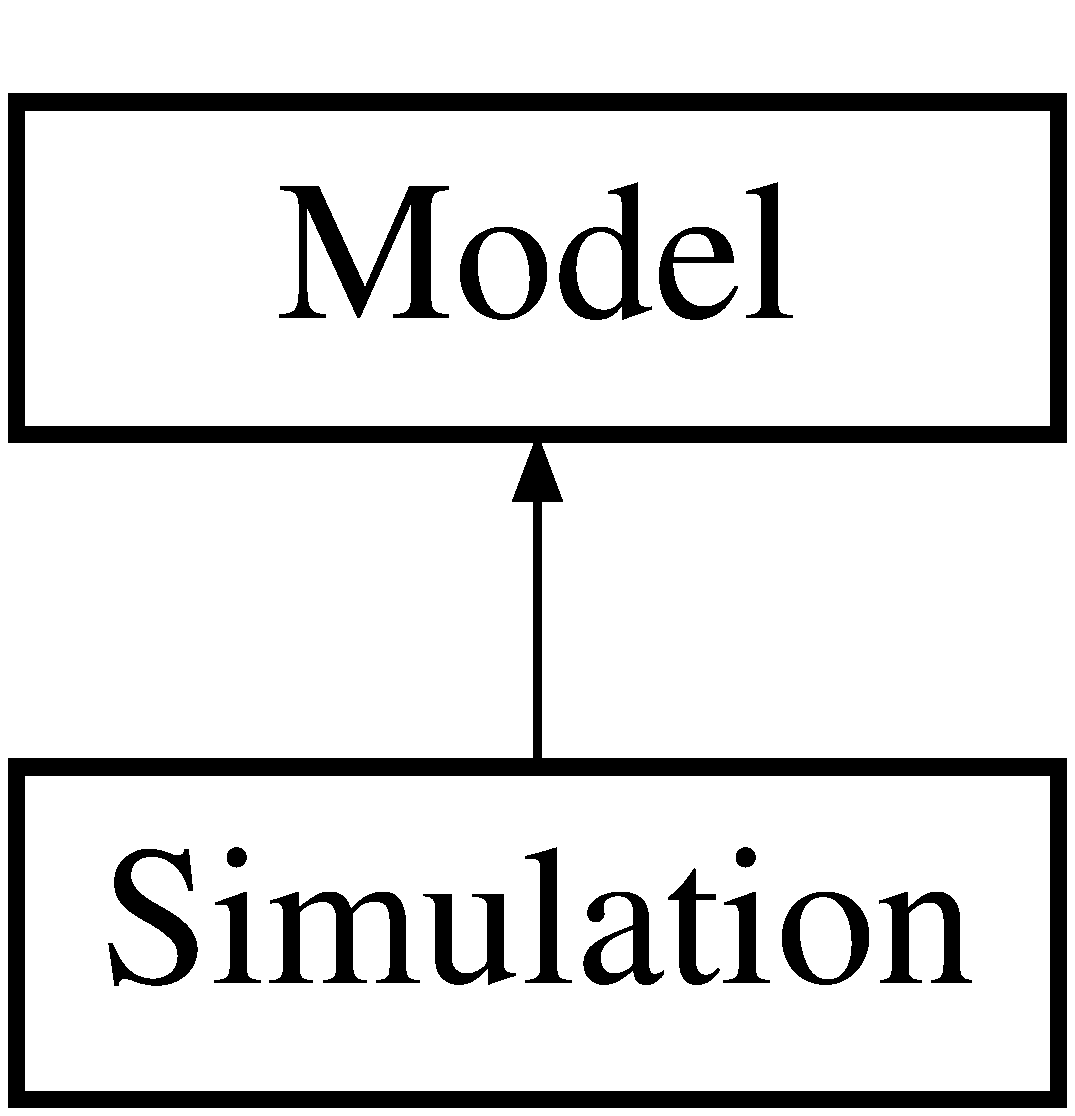
\includegraphics[height=2.000000cm]{structModel}
\end{center}
\end{figure}
\subsection*{Public Member Functions}
\begin{DoxyCompactItemize}
\item 
int \mbox{\hyperlink{structModel_a890018e455118fa3e77def90f280dc52}{read}} (const \mbox{\hyperlink{structIo}{Io}} \&io)
\item 
int \mbox{\hyperlink{structModel_a2d851441d0343b15e8e5affd2f786678}{write}} (const \mbox{\hyperlink{structIo}{Io}} \&io) const
\end{DoxyCompactItemize}
\subsection*{Public Attributes}
\begin{DoxyCompactItemize}
\item 
\mbox{\Hypertarget{structModel_a648f41608b8f8a859e1b00ddf4640414}\label{structModel_a648f41608b8f8a859e1b00ddf4640414}} 
\mbox{\hyperlink{classParameters}{Parameters}} {\bfseries parameters}
\item 
\mbox{\Hypertarget{structModel_a9eac0359f751ae78cbfe52497465f91d}\label{structModel_a9eac0359f751ae78cbfe52497465f91d}} 
\mbox{\hyperlink{structGeometry}{Geometry}} {\bfseries geometry}
\item 
\mbox{\Hypertarget{structModel_ab371cdf43cb5dc99c968daaf4a492a7a}\label{structModel_ab371cdf43cb5dc99c968daaf4a492a7a}} 
\mbox{\hyperlink{structChemistry}{Chemistry}} {\bfseries chemistry}
\item 
\mbox{\Hypertarget{structModel_ac5a521af88897ede48b542c798137580}\label{structModel_ac5a521af88897ede48b542c798137580}} 
\mbox{\hyperlink{structLines}{Lines}} {\bfseries lines}
\item 
\mbox{\Hypertarget{structModel_a534b5df30d90b66521e0bf7c1a517447}\label{structModel_a534b5df30d90b66521e0bf7c1a517447}} 
\mbox{\hyperlink{structThermodynamics}{Thermodynamics}} {\bfseries thermodynamics}
\item 
\mbox{\Hypertarget{structModel_a1a6983c58adaf88fab7cdfbd5a8ecd71}\label{structModel_a1a6983c58adaf88fab7cdfbd5a8ecd71}} 
\mbox{\hyperlink{structRadiation}{Radiation}} {\bfseries radiation}
\end{DoxyCompactItemize}


\subsection{Detailed Description}
\mbox{\hyperlink{structModel}{Model}}\+: a distributed data structure for Magritte\textquotesingle{}s model data. 

\subsection{Member Function Documentation}
\mbox{\Hypertarget{structModel_a890018e455118fa3e77def90f280dc52}\label{structModel_a890018e455118fa3e77def90f280dc52}} 
\index{Model@{Model}!read@{read}}
\index{read@{read}!Model@{Model}}
\subsubsection{\texorpdfstring{read()}{read()}}
{\footnotesize\ttfamily int Model\+::read (\begin{DoxyParamCaption}\item[{const \mbox{\hyperlink{structIo}{Io}} \&}]{io }\end{DoxyParamCaption})}

read\+: read model data 
\begin{DoxyParams}[1]{Parameters}
\mbox{\tt in}  & {\em io} & io data object \\
\hline
\end{DoxyParams}
\mbox{\Hypertarget{structModel_a2d851441d0343b15e8e5affd2f786678}\label{structModel_a2d851441d0343b15e8e5affd2f786678}} 
\index{Model@{Model}!write@{write}}
\index{write@{write}!Model@{Model}}
\subsubsection{\texorpdfstring{write()}{write()}}
{\footnotesize\ttfamily int Model\+::write (\begin{DoxyParamCaption}\item[{const \mbox{\hyperlink{structIo}{Io}} \&}]{io }\end{DoxyParamCaption}) const}

write\+: write out model data 
\begin{DoxyParams}[1]{Parameters}
\mbox{\tt in}  & {\em io} & io data object \\
\hline
\end{DoxyParams}


The documentation for this struct was generated from the following files\+:\begin{DoxyCompactItemize}
\item 
/home/frederik/\+Dropbox/\+Astro/\+Magritte/src/\+Model/model.\+hpp\item 
/home/frederik/\+Dropbox/\+Astro/\+Magritte/src/\+Model/model.\+cpp\end{DoxyCompactItemize}

\hypertarget{classMPI__TIMER}{}\section{M\+P\+I\+\_\+\+T\+I\+M\+ER Class Reference}
\label{classMPI__TIMER}\index{M\+P\+I\+\_\+\+T\+I\+M\+ER@{M\+P\+I\+\_\+\+T\+I\+M\+ER}}


\mbox{\hyperlink{classMPI__TIMER}{M\+P\+I\+\_\+\+T\+I\+M\+ER}}\+: class for precise process timing when using M\+PI.  




{\ttfamily \#include $<$timer.\+hpp$>$}

\subsection*{Public Member Functions}
\begin{DoxyCompactItemize}
\item 
\mbox{\Hypertarget{classMPI__TIMER_a988e600893d6827710aa28754c663b18}\label{classMPI__TIMER_a988e600893d6827710aa28754c663b18}} 
\mbox{\hyperlink{classMPI__TIMER_a988e600893d6827710aa28754c663b18}{M\+P\+I\+\_\+\+T\+I\+M\+ER}} (string timer\+\_\+name)
\begin{DoxyCompactList}\small\item\em Constructor for \mbox{\hyperlink{classTIMER}{T\+I\+M\+ER}}. \end{DoxyCompactList}\item 
\mbox{\Hypertarget{classMPI__TIMER_a17ed1a36df48a47d91486f570f58eda2}\label{classMPI__TIMER_a17ed1a36df48a47d91486f570f58eda2}} 
void \mbox{\hyperlink{classMPI__TIMER_a17ed1a36df48a47d91486f570f58eda2}{start}} ()
\begin{DoxyCompactList}\small\item\em start\+: start timer i.\+e. set initial time stamp \end{DoxyCompactList}\item 
\mbox{\Hypertarget{classMPI__TIMER_a8d31cf80e1e01f6d96cf1ff35cdce2b2}\label{classMPI__TIMER_a8d31cf80e1e01f6d96cf1ff35cdce2b2}} 
void \mbox{\hyperlink{classMPI__TIMER_a8d31cf80e1e01f6d96cf1ff35cdce2b2}{stop}} ()
\begin{DoxyCompactList}\small\item\em stop\+: stop timer and calculate interval for every process \end{DoxyCompactList}\item 
void \mbox{\hyperlink{classMPI__TIMER_ae2b9502ad9811560bbab8032f8858b16}{print\+\_\+to\+\_\+file}} ()
\item 
\mbox{\Hypertarget{classMPI__TIMER_ada0b12d22f4d9b29730bbce69d894306}\label{classMPI__TIMER_ada0b12d22f4d9b29730bbce69d894306}} 
void \mbox{\hyperlink{classMPI__TIMER_ada0b12d22f4d9b29730bbce69d894306}{print}} ()
\begin{DoxyCompactList}\small\item\em print\+: let rank 0 process print times for every rank \end{DoxyCompactList}\end{DoxyCompactItemize}


\subsection{Detailed Description}
\mbox{\hyperlink{classMPI__TIMER}{M\+P\+I\+\_\+\+T\+I\+M\+ER}}\+: class for precise process timing when using M\+PI. 

\subsection{Member Function Documentation}
\mbox{\Hypertarget{classMPI__TIMER_ae2b9502ad9811560bbab8032f8858b16}\label{classMPI__TIMER_ae2b9502ad9811560bbab8032f8858b16}} 
\index{M\+P\+I\+\_\+\+T\+I\+M\+ER@{M\+P\+I\+\_\+\+T\+I\+M\+ER}!print\+\_\+to\+\_\+file@{print\+\_\+to\+\_\+file}}
\index{print\+\_\+to\+\_\+file@{print\+\_\+to\+\_\+file}!M\+P\+I\+\_\+\+T\+I\+M\+ER@{M\+P\+I\+\_\+\+T\+I\+M\+ER}}
\subsubsection{\texorpdfstring{print\+\_\+to\+\_\+file()}{print\_to\_file()}}
{\footnotesize\ttfamily void M\+P\+I\+\_\+\+T\+I\+M\+E\+R\+::print\+\_\+to\+\_\+file (\begin{DoxyParamCaption}{ }\end{DoxyParamCaption})\hspace{0.3cm}{\ttfamily [inline]}}

print\+\_\+to\+\_\+file\+: let rank 0 process print times for every rank to file 
\begin{DoxyParams}[1]{Parameters}
\mbox{\tt in}  & {\em file\+\_\+name} & name of the file to print to \\
\hline
\end{DoxyParams}


The documentation for this class was generated from the following file\+:\begin{DoxyCompactItemize}
\item 
/home/frederik/\+Dropbox/\+Astro/\+Magritte/src/\+Tools/timer.\+hpp\end{DoxyCompactItemize}

\hypertarget{classParameters}{}\section{Parameters Class Reference}
\label{classParameters}\index{Parameters@{Parameters}}


\mbox{\hyperlink{classParameters}{Parameters}}\+: secure structure for the model parameters.  




{\ttfamily \#include $<$parameters.\+hpp$>$}

\subsection*{Public Member Functions}
\begin{DoxyCompactItemize}
\item 
\mbox{\Hypertarget{classParameters_a62a78a811449d5eae3f7dd0b6426b3e5}\label{classParameters_a62a78a811449d5eae3f7dd0b6426b3e5}} 
void {\bfseries set\+\_\+ncells} (const long value)
\item 
\mbox{\Hypertarget{classParameters_a9897caabb65e87e4c934179c4a21b8b2}\label{classParameters_a9897caabb65e87e4c934179c4a21b8b2}} 
void {\bfseries set\+\_\+ncameras} (const long value)
\item 
\mbox{\Hypertarget{classParameters_a91c99ccecbc13e9502424284639f97f9}\label{classParameters_a91c99ccecbc13e9502424284639f97f9}} 
void {\bfseries set\+\_\+nrays} (const long value)
\item 
\mbox{\Hypertarget{classParameters_a37cd7ed199e2881848d392ff5868e6bb}\label{classParameters_a37cd7ed199e2881848d392ff5868e6bb}} 
void {\bfseries set\+\_\+nrays\+\_\+red} (const long value)
\item 
\mbox{\Hypertarget{classParameters_a74485125ea038240b2eb54780961c970}\label{classParameters_a74485125ea038240b2eb54780961c970}} 
void {\bfseries set\+\_\+nboundary} (const long value)
\item 
\mbox{\Hypertarget{classParameters_a5626c4070761626dc2765cb7791798fa}\label{classParameters_a5626c4070761626dc2765cb7791798fa}} 
void {\bfseries set\+\_\+nfreqs} (const long value)
\item 
\mbox{\Hypertarget{classParameters_ac01bc63944bdadeb86d8664537d0febe}\label{classParameters_ac01bc63944bdadeb86d8664537d0febe}} 
void {\bfseries set\+\_\+nfreqs\+\_\+red} (const long value)
\item 
\mbox{\Hypertarget{classParameters_adf5f01e44bf7d5df59d6010fb9782afb}\label{classParameters_adf5f01e44bf7d5df59d6010fb9782afb}} 
void {\bfseries set\+\_\+nspecs} (const long value)
\item 
\mbox{\Hypertarget{classParameters_a2661a3dbd765a9d2af876470d34dbae2}\label{classParameters_a2661a3dbd765a9d2af876470d34dbae2}} 
void {\bfseries set\+\_\+nlspecs} (const long value)
\item 
\mbox{\Hypertarget{classParameters_abaa5011b841c89ba28ac0e884003ff87}\label{classParameters_abaa5011b841c89ba28ac0e884003ff87}} 
void {\bfseries set\+\_\+nlines} (const long value)
\item 
\mbox{\Hypertarget{classParameters_ac505977b196477ab248450ef6ec32b53}\label{classParameters_ac505977b196477ab248450ef6ec32b53}} 
void {\bfseries set\+\_\+nquads} (const long value)
\item 
\mbox{\Hypertarget{classParameters_a6b57ecff227f0cdb00b450a6e6ef0b15}\label{classParameters_a6b57ecff227f0cdb00b450a6e6ef0b15}} 
void {\bfseries set\+\_\+pop\+\_\+prec} (const double value)
\item 
\mbox{\Hypertarget{classParameters_ae51213e1215d5726d2ae7c750ca02a42}\label{classParameters_ae51213e1215d5726d2ae7c750ca02a42}} 
void {\bfseries set\+\_\+use\+\_\+scattering} (const bool value)
\item 
\mbox{\Hypertarget{classParameters_a5a0e60bfdbb1251a95633bc13c98edce}\label{classParameters_a5a0e60bfdbb1251a95633bc13c98edce}} 
void {\bfseries set\+\_\+use\+\_\+\+Ng\+\_\+acceleration} (const bool value)
\item 
\mbox{\Hypertarget{classParameters_a9a11a2bca19314d9695a5779613e9df1}\label{classParameters_a9a11a2bca19314d9695a5779613e9df1}} 
long {\bfseries ncells} (void) const
\item 
\mbox{\Hypertarget{classParameters_a2b531cdc89dc6123ceafb91480b1b419}\label{classParameters_a2b531cdc89dc6123ceafb91480b1b419}} 
long {\bfseries ncameras} (void) const
\item 
\mbox{\Hypertarget{classParameters_a15904d79702bcd72b73fb2049b8f1487}\label{classParameters_a15904d79702bcd72b73fb2049b8f1487}} 
long {\bfseries nrays} (void) const
\item 
\mbox{\Hypertarget{classParameters_a9d15d3cd204c374edb7f9d5797b3d06a}\label{classParameters_a9d15d3cd204c374edb7f9d5797b3d06a}} 
long {\bfseries nrays\+\_\+red} (void) const
\item 
\mbox{\Hypertarget{classParameters_a3c0519629ec48c9003e599c168f72f26}\label{classParameters_a3c0519629ec48c9003e599c168f72f26}} 
long {\bfseries nboundary} (void) const
\item 
\mbox{\Hypertarget{classParameters_a54cc7ff6fd465c9d3f873455edec7136}\label{classParameters_a54cc7ff6fd465c9d3f873455edec7136}} 
long {\bfseries nfreqs} (void) const
\item 
\mbox{\Hypertarget{classParameters_aea06a149efe7e431720e09d9d8b0b70d}\label{classParameters_aea06a149efe7e431720e09d9d8b0b70d}} 
long {\bfseries nfreqs\+\_\+red} (void) const
\item 
\mbox{\Hypertarget{classParameters_aaaebc90313dd5c9cadfc5889f448b89b}\label{classParameters_aaaebc90313dd5c9cadfc5889f448b89b}} 
long {\bfseries nspecs} (void) const
\item 
\mbox{\Hypertarget{classParameters_a8351d3b3fa555c59943ee27072612962}\label{classParameters_a8351d3b3fa555c59943ee27072612962}} 
long {\bfseries nlspecs} (void) const
\item 
\mbox{\Hypertarget{classParameters_a13594666258a61680b3d77efcebf86c7}\label{classParameters_a13594666258a61680b3d77efcebf86c7}} 
long {\bfseries nlines} (void) const
\item 
\mbox{\Hypertarget{classParameters_a4d7a96a332aa99994c08dc05d8895ff4}\label{classParameters_a4d7a96a332aa99994c08dc05d8895ff4}} 
long {\bfseries nquads} (void) const
\item 
\mbox{\Hypertarget{classParameters_abef0cfc7dab680e9533f183bb3176a52}\label{classParameters_abef0cfc7dab680e9533f183bb3176a52}} 
double {\bfseries pop\+\_\+prec} (void) const
\item 
\mbox{\Hypertarget{classParameters_aa04a263e330fc6a5197196c51aa20235}\label{classParameters_aa04a263e330fc6a5197196c51aa20235}} 
bool {\bfseries use\+\_\+scattering} (void) const
\item 
\mbox{\Hypertarget{classParameters_a5adb7b4e2485e753d0ece86ed52ba8f5}\label{classParameters_a5adb7b4e2485e753d0ece86ed52ba8f5}} 
bool {\bfseries use\+\_\+\+Ng\+\_\+acceleration} (void) const
\item 
\mbox{\Hypertarget{classParameters_a3ed5e956a8c6778200ffc8eaf478c23c}\label{classParameters_a3ed5e956a8c6778200ffc8eaf478c23c}} 
int {\bfseries read} (const \mbox{\hyperlink{structIo}{Io}} \&io)
\item 
\mbox{\Hypertarget{classParameters_a6dee8e9f938079d64494e5b5f0eff16f}\label{classParameters_a6dee8e9f938079d64494e5b5f0eff16f}} 
int {\bfseries write} (const \mbox{\hyperlink{structIo}{Io}} \&io) const
\end{DoxyCompactItemize}
\subsection*{Public Attributes}
\begin{DoxyCompactItemize}
\item 
\mbox{\Hypertarget{classParameters_a0cff5f349621c95ed87d10db2a64520d}\label{classParameters_a0cff5f349621c95ed87d10db2a64520d}} 
long {\bfseries r}
\item 
\mbox{\Hypertarget{classParameters_a8fa1130d41666c907c9f8ec993374fc3}\label{classParameters_a8fa1130d41666c907c9f8ec993374fc3}} 
long {\bfseries o}
\item 
\mbox{\Hypertarget{classParameters_a364ff2e8cafed3be6c00c8b709d6ed31}\label{classParameters_a364ff2e8cafed3be6c00c8b709d6ed31}} 
long {\bfseries f}
\item 
\mbox{\Hypertarget{classParameters_af147c2a5b9ed14cf18c8d61cd63cc4f3}\label{classParameters_af147c2a5b9ed14cf18c8d61cd63cc4f3}} 
long {\bfseries n\+\_\+off\+\_\+diag} = 0
\item 
\mbox{\Hypertarget{classParameters_af07bf93fa81400773c457787e11fe903}\label{classParameters_af07bf93fa81400773c457787e11fe903}} 
double {\bfseries max\+\_\+width\+\_\+fraction} = 0.\+5
\end{DoxyCompactItemize}


\subsection{Detailed Description}
\mbox{\hyperlink{classParameters}{Parameters}}\+: secure structure for the model parameters. 

The documentation for this class was generated from the following files\+:\begin{DoxyCompactItemize}
\item 
/home/frederik/\+Dropbox/\+Astro/\+Magritte/src/\+Model/parameters.\+hpp\item 
/home/frederik/\+Dropbox/\+Astro/\+Magritte/src/\+Model/parameters.\+cpp\end{DoxyCompactItemize}

\hypertarget{structProjectedCellData}{}\section{Projected\+Cell\+Data Struct Reference}
\label{structProjectedCellData}\index{Projected\+Cell\+Data@{Projected\+Cell\+Data}}


\mbox{\hyperlink{structProjectedCellData}{Projected\+Cell\+Data}}\+: data structure for the data projected on a ray.  




{\ttfamily \#include $<$raydata.\+hpp$>$}

\subsection*{Public Attributes}
\begin{DoxyCompactItemize}
\item 
\mbox{\Hypertarget{structProjectedCellData_a13fdb833344863717d217129ec398f2e}\label{structProjectedCellData_a13fdb833344863717d217129ec398f2e}} 
long {\bfseries cell\+Nr}
\item 
\mbox{\Hypertarget{structProjectedCellData_ab311bd5ac07266244dc820384dc15ad9}\label{structProjectedCellData_ab311bd5ac07266244dc820384dc15ad9}} 
double {\bfseries shift}
\item 
\mbox{\Hypertarget{structProjectedCellData_a6f6743f346f2e10a0ae08fc826850575}\label{structProjectedCellData_a6f6743f346f2e10a0ae08fc826850575}} 
double {\bfseries dZ}
\item 
\mbox{\Hypertarget{structProjectedCellData_a69e758a7e32926d242edcc31c5e49d82}\label{structProjectedCellData_a69e758a7e32926d242edcc31c5e49d82}} 
long {\bfseries lnotch}
\item 
\mbox{\Hypertarget{structProjectedCellData_aba13abdae8f496ef0dfffefc5c19b64f}\label{structProjectedCellData_aba13abdae8f496ef0dfffefc5c19b64f}} 
long {\bfseries notch}
\end{DoxyCompactItemize}


\subsection{Detailed Description}
\mbox{\hyperlink{structProjectedCellData}{Projected\+Cell\+Data}}\+: data structure for the data projected on a ray. 

The documentation for this struct was generated from the following file\+:\begin{DoxyCompactItemize}
\item 
/home/frederik/\+Dropbox/\+Astro/\+Magritte/src/\+Model/\+Geometry/raydata.\+hpp\end{DoxyCompactItemize}

\hypertarget{structQuadrature}{}\section{Quadrature Struct Reference}
\label{structQuadrature}\index{Quadrature@{Quadrature}}
\subsection*{Public Member Functions}
\begin{DoxyCompactItemize}
\item 
int \mbox{\hyperlink{structQuadrature_a8a5353ea2b41c9ca21ba6c48e019678c}{read}} (const \mbox{\hyperlink{structIo}{Io}} \&io, const int l, \mbox{\hyperlink{classParameters}{Parameters}} \&parameters)
\item 
int \mbox{\hyperlink{structQuadrature_ae7cd1922b845cdb79ad3bbf89e4e2c81}{write}} (const \mbox{\hyperlink{structIo}{Io}} \&io, const int l) const
\end{DoxyCompactItemize}
\subsection*{Public Attributes}
\begin{DoxyCompactItemize}
\item 
\mbox{\Hypertarget{structQuadrature_ab8bb181e2754ed8b1098e19b7de45d26}\label{structQuadrature_ab8bb181e2754ed8b1098e19b7de45d26}} 
Double1 {\bfseries roots}
\item 
\mbox{\Hypertarget{structQuadrature_a4eabe98a84a5757b08beda3604cb9ab8}\label{structQuadrature_a4eabe98a84a5757b08beda3604cb9ab8}} 
Double1 {\bfseries weights}
\end{DoxyCompactItemize}


\subsection{Member Function Documentation}
\mbox{\Hypertarget{structQuadrature_a8a5353ea2b41c9ca21ba6c48e019678c}\label{structQuadrature_a8a5353ea2b41c9ca21ba6c48e019678c}} 
\index{Quadrature@{Quadrature}!read@{read}}
\index{read@{read}!Quadrature@{Quadrature}}
\subsubsection{\texorpdfstring{read()}{read()}}
{\footnotesize\ttfamily int Quadrature\+::read (\begin{DoxyParamCaption}\item[{const \mbox{\hyperlink{structIo}{Io}} \&}]{io,  }\item[{const int}]{l,  }\item[{\mbox{\hyperlink{classParameters}{Parameters}} \&}]{parameters }\end{DoxyParamCaption})}

read\+: read in data structure 
\begin{DoxyParams}[1]{Parameters}
\mbox{\tt in}  & {\em io} & io object \\
\hline
\mbox{\tt in}  & {\em parameters} & model parameters object \\
\hline
\end{DoxyParams}
\mbox{\Hypertarget{structQuadrature_ae7cd1922b845cdb79ad3bbf89e4e2c81}\label{structQuadrature_ae7cd1922b845cdb79ad3bbf89e4e2c81}} 
\index{Quadrature@{Quadrature}!write@{write}}
\index{write@{write}!Quadrature@{Quadrature}}
\subsubsection{\texorpdfstring{write()}{write()}}
{\footnotesize\ttfamily int Quadrature\+::write (\begin{DoxyParamCaption}\item[{const \mbox{\hyperlink{structIo}{Io}} \&}]{io,  }\item[{const int}]{l }\end{DoxyParamCaption}) const}

write\+: write out data structure 
\begin{DoxyParams}[1]{Parameters}
\mbox{\tt in}  & {\em io} & io object \\
\hline
\end{DoxyParams}


The documentation for this struct was generated from the following files\+:\begin{DoxyCompactItemize}
\item 
/home/frederik/\+Dropbox/\+Astro/\+Magritte/src/\+Model/\+Lines/\+Line\+Producing\+Species/\+Quadrature/quadrature.\+hpp\item 
/home/frederik/\+Dropbox/\+Astro/\+Magritte/src/\+Model/\+Lines/\+Line\+Producing\+Species/\+Quadrature/quadrature.\+cpp\end{DoxyCompactItemize}

\hypertarget{structRadiation}{}\section{Radiation Struct Reference}
\label{structRadiation}\index{Radiation@{Radiation}}


\mbox{\hyperlink{structRadiation}{Radiation}}\+: data structure for the radiation field.  




{\ttfamily \#include $<$radiation.\+hpp$>$}

\subsection*{Public Member Functions}
\begin{DoxyCompactItemize}
\item 
int \mbox{\hyperlink{structRadiation_ae1c20ca666229715888324bdfc7e7b32}{read}} (const \mbox{\hyperlink{structIo}{Io}} \&io, \mbox{\hyperlink{classParameters}{Parameters}} \&parameters)
\item 
int \mbox{\hyperlink{structRadiation_adb8acb48bb764b2dce1b4060f8ded541}{write}} (const \mbox{\hyperlink{structIo}{Io}} \&io) const
\item 
\mbox{\Hypertarget{structRadiation_a9d0c9c1b51c28bf6a3eda363a0b84327}\label{structRadiation_a9d0c9c1b51c28bf6a3eda363a0b84327}} 
long {\bfseries index} (const long p, const long f) const
\item 
\mbox{\Hypertarget{structRadiation_af7a62862349300f6983e65ea6286844f}\label{structRadiation_af7a62862349300f6983e65ea6286844f}} 
long {\bfseries index} (const long p, const long f, const long m) const
\item 
\mbox{\Hypertarget{structRadiation_a9712eac769f8adb4c8bc39ef1d3b7dcd}\label{structRadiation_a9712eac769f8adb4c8bc39ef1d3b7dcd}} 
v\+Real {\bfseries get\+\_\+U} (const long R, const long p, const long f) const
\item 
\mbox{\Hypertarget{structRadiation_ad12ee819315cf5400895c12d84ca8fe2}\label{structRadiation_ad12ee819315cf5400895c12d84ca8fe2}} 
v\+Real {\bfseries get\+\_\+V} (const long R, const long p, const long f) const
\item 
\mbox{\Hypertarget{structRadiation_af35d4cf35915a0d8ad02f0cbb1c89c63}\label{structRadiation_af35d4cf35915a0d8ad02f0cbb1c89c63}} 
v\+Real {\bfseries get\+\_\+\+I\+\_\+bdy} (const long R, const long p, const long f) const
\item 
\mbox{\Hypertarget{structRadiation_aa006c2c220fb0f9613ca9b7697dd2474}\label{structRadiation_aa006c2c220fb0f9613ca9b7697dd2474}} 
void {\bfseries rescale\+\_\+\+U\+\_\+and\+\_\+V} (const v\+Real \&freq\+\_\+scaled, const long R, const long p, long \&notch, v\+Real \&U\+\_\+scaled, v\+Real \&V\+\_\+scaled) const
\item 
\mbox{\Hypertarget{structRadiation_a36dcce5059f8d6f14c24feb06a1d52c4}\label{structRadiation_a36dcce5059f8d6f14c24feb06a1d52c4}} 
void {\bfseries rescale\+\_\+\+I\+\_\+bdy} (const v\+Real \&freq\+\_\+scaled, const long R, const long p, const long b, long \&notch, v\+Real \&Ibdy\+\_\+scaled) const
\item 
\mbox{\Hypertarget{structRadiation_ad6c8c7bf0a4f451f29e053000bf4fa04}\label{structRadiation_ad6c8c7bf0a4f451f29e053000bf4fa04}} 
int {\bfseries initialize\+\_\+J} ()
\item 
int \mbox{\hyperlink{structRadiation_a70b08565e0721c6b190cd161c6214368}{M\+P\+I\+\_\+reduce\+\_\+J}} ()
\begin{DoxyCompactList}\small\item\em mpi\+\_\+vector\+\_\+sum\+: custom reduction operation for M\+P\+I\+\_\+\+Reduce \end{DoxyCompactList}\item 
\mbox{\Hypertarget{structRadiation_ad776dfdbd3d12eda801ea58648f68246}\label{structRadiation_ad776dfdbd3d12eda801ea58648f68246}} 
int \mbox{\hyperlink{structRadiation_ad776dfdbd3d12eda801ea58648f68246}{calc\+\_\+\+U\+\_\+and\+\_\+V}} ()
\begin{DoxyCompactList}\small\item\em calc\+\_\+\+U\+\_\+and\+\_\+V\+: integrate scattering quantities over all directions \end{DoxyCompactList}\end{DoxyCompactItemize}
\subsection*{Public Attributes}
\begin{DoxyCompactItemize}
\item 
\mbox{\Hypertarget{structRadiation_a671301011aedcded797ed7380b8e62d2}\label{structRadiation_a671301011aedcded797ed7380b8e62d2}} 
\mbox{\hyperlink{structFrequencies}{Frequencies}} {\bfseries frequencies}
\item 
\mbox{\Hypertarget{structRadiation_a2312d1d46d0091dd9e03beeeda186943}\label{structRadiation_a2312d1d46d0091dd9e03beeeda186943}} 
\mbox{\hyperlink{structScattering}{Scattering}} {\bfseries scattering}
\item 
\mbox{\Hypertarget{structRadiation_adb6e1c2c5c515af5568f7426d74494db}\label{structRadiation_adb6e1c2c5c515af5568f7426d74494db}} 
v\+Real2 \mbox{\hyperlink{structRadiation_adb6e1c2c5c515af5568f7426d74494db}{u}}
\begin{DoxyCompactList}\small\item\em u intensity (r, index(p,f)) \end{DoxyCompactList}\item 
\mbox{\Hypertarget{structRadiation_a00797002bf4209bb24c1c8bb95f86375}\label{structRadiation_a00797002bf4209bb24c1c8bb95f86375}} 
v\+Real2 \mbox{\hyperlink{structRadiation_a00797002bf4209bb24c1c8bb95f86375}{v}}
\begin{DoxyCompactList}\small\item\em v intensity (r, index(p,f)) \end{DoxyCompactList}\item 
\mbox{\Hypertarget{structRadiation_a82c337ae7b2a51d06b36dac7a1b256ea}\label{structRadiation_a82c337ae7b2a51d06b36dac7a1b256ea}} 
v\+Real2 \mbox{\hyperlink{structRadiation_a82c337ae7b2a51d06b36dac7a1b256ea}{U}}
\begin{DoxyCompactList}\small\item\em U scattered intensity (r, index(p,f)) \end{DoxyCompactList}\item 
\mbox{\Hypertarget{structRadiation_a9012339ab0e070b9e5e5ae9b2f3acc13}\label{structRadiation_a9012339ab0e070b9e5e5ae9b2f3acc13}} 
v\+Real2 \mbox{\hyperlink{structRadiation_a9012339ab0e070b9e5e5ae9b2f3acc13}{V}}
\begin{DoxyCompactList}\small\item\em V scattered intensity (r, index(p,f)) \end{DoxyCompactList}\item 
\mbox{\Hypertarget{structRadiation_affdd4d2724f5d0b74c51ed6577b138b3}\label{structRadiation_affdd4d2724f5d0b74c51ed6577b138b3}} 
v\+Real1 \mbox{\hyperlink{structRadiation_affdd4d2724f5d0b74c51ed6577b138b3}{J}}
\begin{DoxyCompactList}\small\item\em (angular) mean intensity (index(p,f)) \end{DoxyCompactList}\item 
\mbox{\Hypertarget{structRadiation_a15149e3b370f8c7efff1784acfaa4e59}\label{structRadiation_a15149e3b370f8c7efff1784acfaa4e59}} 
v\+Real3 \mbox{\hyperlink{structRadiation_a15149e3b370f8c7efff1784acfaa4e59}{I\+\_\+bdy}}
\begin{DoxyCompactList}\small\item\em intensity at the boundary (r,b,f) \end{DoxyCompactList}\end{DoxyCompactItemize}


\subsection{Detailed Description}
\mbox{\hyperlink{structRadiation}{Radiation}}\+: data structure for the radiation field. 

\subsection{Member Function Documentation}
\mbox{\Hypertarget{structRadiation_a70b08565e0721c6b190cd161c6214368}\label{structRadiation_a70b08565e0721c6b190cd161c6214368}} 
\index{Radiation@{Radiation}!M\+P\+I\+\_\+reduce\+\_\+J@{M\+P\+I\+\_\+reduce\+\_\+J}}
\index{M\+P\+I\+\_\+reduce\+\_\+J@{M\+P\+I\+\_\+reduce\+\_\+J}!Radiation@{Radiation}}
\subsubsection{\texorpdfstring{M\+P\+I\+\_\+reduce\+\_\+\+J()}{MPI\_reduce\_J()}}
{\footnotesize\ttfamily int Radiation\+::\+M\+P\+I\+\_\+reduce\+\_\+J (\begin{DoxyParamCaption}{ }\end{DoxyParamCaption})}



mpi\+\_\+vector\+\_\+sum\+: custom reduction operation for M\+P\+I\+\_\+\+Reduce 

calc\+\_\+J\+: integrate mean intensity and "flux over all directions \mbox{\Hypertarget{structRadiation_ae1c20ca666229715888324bdfc7e7b32}\label{structRadiation_ae1c20ca666229715888324bdfc7e7b32}} 
\index{Radiation@{Radiation}!read@{read}}
\index{read@{read}!Radiation@{Radiation}}
\subsubsection{\texorpdfstring{read()}{read()}}
{\footnotesize\ttfamily int Radiation\+::read (\begin{DoxyParamCaption}\item[{const \mbox{\hyperlink{structIo}{Io}} \&}]{io,  }\item[{\mbox{\hyperlink{classParameters}{Parameters}} \&}]{parameters }\end{DoxyParamCaption})}

read\+: read in data structure 
\begin{DoxyParams}[1]{Parameters}
\mbox{\tt in}  & {\em io} & io object \\
\hline
\mbox{\tt in}  & {\em parameters} & model parameters object \\
\hline
\end{DoxyParams}
\mbox{\Hypertarget{structRadiation_adb8acb48bb764b2dce1b4060f8ded541}\label{structRadiation_adb8acb48bb764b2dce1b4060f8ded541}} 
\index{Radiation@{Radiation}!write@{write}}
\index{write@{write}!Radiation@{Radiation}}
\subsubsection{\texorpdfstring{write()}{write()}}
{\footnotesize\ttfamily int Radiation\+::write (\begin{DoxyParamCaption}\item[{const \mbox{\hyperlink{structIo}{Io}} \&}]{io }\end{DoxyParamCaption}) const}

write\+: write out data structure 
\begin{DoxyParams}[1]{Parameters}
\mbox{\tt in}  & {\em io} & io object \\
\hline
\end{DoxyParams}


The documentation for this struct was generated from the following files\+:\begin{DoxyCompactItemize}
\item 
/home/frederik/\+Dropbox/\+Astro/\+Magritte/src/\+Model/\+Radiation/radiation.\+hpp\item 
/home/frederik/\+Dropbox/\+Astro/\+Magritte/src/\+Model/\+Radiation/radiation.\+cpp\end{DoxyCompactItemize}

\hypertarget{structRayPair}{}\section{Ray\+Pair Struct Reference}
\label{structRayPair}\index{Ray\+Pair@{Ray\+Pair}}


Raypair\+: data structure for a pair of rays.  




{\ttfamily \#include $<$raypair.\+hpp$>$}

\subsection*{Public Member Functions}
\begin{DoxyCompactItemize}
\item 
\mbox{\Hypertarget{structRayPair_aadb079089f5d5d230e26ecb00d3802cc}\label{structRayPair_aadb079089f5d5d230e26ecb00d3802cc}} 
void {\bfseries initialize} (const long n\+\_\+ar, const long n\+\_\+r)
\item 
\mbox{\Hypertarget{structRayPair_a65f67e4d6a83dbfc2d8fe5a2520cd678}\label{structRayPair_a65f67e4d6a83dbfc2d8fe5a2520cd678}} 
void {\bfseries solve} ()
\item 
\mbox{\Hypertarget{structRayPair_ac79352ff8e893cff0a5d752da4337a70}\label{structRayPair_ac79352ff8e893cff0a5d752da4337a70}} 
void {\bfseries set\+\_\+term1\+\_\+and\+\_\+term2} (const v\+Real \&eta, const v\+Real \&chi, const v\+Real \&U\+\_\+scaled, const v\+Real \&V\+\_\+scaled, const long n)
\item 
\mbox{\Hypertarget{structRayPair_a509c43c4a1682d360e16ae1818520ed0}\label{structRayPair_a509c43c4a1682d360e16ae1818520ed0}} 
void {\bfseries set\+\_\+dtau} (const v\+Real \&chi, const v\+Real \&chi\+\_\+prev, const double dZ, const long n)
\item 
\mbox{\Hypertarget{structRayPair_a25a21ab5df7a0112284f36e21fa8f9ef}\label{structRayPair_a25a21ab5df7a0112284f36e21fa8f9ef}} 
v\+Real {\bfseries get\+\_\+u\+\_\+at\+\_\+origin} () const
\item 
\mbox{\Hypertarget{structRayPair_a5f3f4f7d73e6ff70f2ef4af897f80000}\label{structRayPair_a5f3f4f7d73e6ff70f2ef4af897f80000}} 
v\+Real {\bfseries get\+\_\+v\+\_\+at\+\_\+origin} () const
\item 
\mbox{\Hypertarget{structRayPair_aa40a22e8fa15929d68201c6f1c01b11a}\label{structRayPair_aa40a22e8fa15929d68201c6f1c01b11a}} 
v\+Real {\bfseries get\+\_\+\+Ip} ()
\item 
\mbox{\Hypertarget{structRayPair_a10e89a2201ee87e2ea5980108056cc09}\label{structRayPair_a10e89a2201ee87e2ea5980108056cc09}} 
v\+Real {\bfseries get\+\_\+\+Im} ()
\item 
\mbox{\Hypertarget{structRayPair_a96f3d8e41ce1a210be44a5bbec2bed0b}\label{structRayPair_a96f3d8e41ce1a210be44a5bbec2bed0b}} 
v\+Real {\bfseries get\+\_\+\+I\+\_\+p} () const
\item 
\mbox{\Hypertarget{structRayPair_a5e925be3d1d2184d31a4f978c618df44}\label{structRayPair_a5e925be3d1d2184d31a4f978c618df44}} 
v\+Real {\bfseries get\+\_\+\+I\+\_\+m} () const
\item 
\mbox{\Hypertarget{structRayPair_a811cf18e0f5401ae9dee6e1bfe4f03eb}\label{structRayPair_a811cf18e0f5401ae9dee6e1bfe4f03eb}} 
double {\bfseries get\+\_\+\+L\+\_\+diag} (const \mbox{\hyperlink{structThermodynamics}{Thermodynamics}} \&thermodynamics, const double inverse\+\_\+mass, const double freq\+\_\+line, const int lane) const
\item 
\mbox{\Hypertarget{structRayPair_a313378a90dc0a63df52281b5becfeaac}\label{structRayPair_a313378a90dc0a63df52281b5becfeaac}} 
double {\bfseries get\+\_\+\+L\+\_\+lower} (const \mbox{\hyperlink{structThermodynamics}{Thermodynamics}} \&thermodynamics, const double inverse\+\_\+mass, const double freq\+\_\+line, const int lane, const long m) const
\item 
\mbox{\Hypertarget{structRayPair_a1c7858e737ddf3204e2f77cdc9d2ac07}\label{structRayPair_a1c7858e737ddf3204e2f77cdc9d2ac07}} 
double {\bfseries get\+\_\+\+L\+\_\+upper} (const \mbox{\hyperlink{structThermodynamics}{Thermodynamics}} \&thermodynamics, const double inverse\+\_\+mass, const double freq\+\_\+line, const int lane, const long m) const
\item 
\mbox{\Hypertarget{structRayPair_a2024d05b8ffe51d56611d28b6af8269c}\label{structRayPair_a2024d05b8ffe51d56611d28b6af8269c}} 
void {\bfseries update\+\_\+\+Lambda} (const \mbox{\hyperlink{structFrequencies}{Frequencies}} \&frequencies, const \mbox{\hyperlink{structThermodynamics}{Thermodynamics}} \&thermodynamics, const long p, const long f, const double weight\+\_\+angular, \mbox{\hyperlink{structLines}{Lines}} \&lines) const
\end{DoxyCompactItemize}
\subsection*{Public Attributes}
\begin{DoxyCompactItemize}
\item 
\mbox{\Hypertarget{structRayPair_a3cd08b2dd78d0aae6f86b0ba8c6803b8}\label{structRayPair_a3cd08b2dd78d0aae6f86b0ba8c6803b8}} 
long {\bfseries n\+\_\+ar}
\item 
\mbox{\Hypertarget{structRayPair_a42151030690e3ba5e5c6eb6238c0f0a7}\label{structRayPair_a42151030690e3ba5e5c6eb6238c0f0a7}} 
long {\bfseries n\+\_\+r}
\item 
\mbox{\Hypertarget{structRayPair_a48a66299e2f6246ad8b9c1cd50005c6c}\label{structRayPair_a48a66299e2f6246ad8b9c1cd50005c6c}} 
long {\bfseries ndep}
\item 
\mbox{\Hypertarget{structRayPair_a0af446588434326eeeb5c3796c27def4}\label{structRayPair_a0af446588434326eeeb5c3796c27def4}} 
v\+Real {\bfseries I\+\_\+bdy\+\_\+0}
\item 
\mbox{\Hypertarget{structRayPair_ab3006c7b67570cd1617fec3ecc7b0d15}\label{structRayPair_ab3006c7b67570cd1617fec3ecc7b0d15}} 
v\+Real {\bfseries I\+\_\+bdy\+\_\+n}
\item 
\mbox{\Hypertarget{structRayPair_a2eefd1eae379f34dbf0f808d7391d64c}\label{structRayPair_a2eefd1eae379f34dbf0f808d7391d64c}} 
long {\bfseries lnotch\+\_\+at\+\_\+origin}
\item 
\mbox{\Hypertarget{structRayPair_a21c3b69a5f0b47402c017cb817ef1100}\label{structRayPair_a21c3b69a5f0b47402c017cb817ef1100}} 
v\+Real1 {\bfseries chi}
\item 
\mbox{\Hypertarget{structRayPair_a9e2e85a1b03bc9ad7384ae7a854d5883}\label{structRayPair_a9e2e85a1b03bc9ad7384ae7a854d5883}} 
Long1 {\bfseries nrs}
\item 
\mbox{\Hypertarget{structRayPair_a1651af5f48ae607cf4bad144ee04f1bf}\label{structRayPair_a1651af5f48ae607cf4bad144ee04f1bf}} 
v\+Real1 {\bfseries frs}
\item 
\mbox{\Hypertarget{structRayPair_af2019296a7f6f823646c6abca3b4bc34}\label{structRayPair_af2019296a7f6f823646c6abca3b4bc34}} 
long {\bfseries n\+\_\+off\+\_\+diag} = 0
\item 
\mbox{\Hypertarget{structRayPair_a58120563ed7fecafa0f2bef33dffd66b}\label{structRayPair_a58120563ed7fecafa0f2bef33dffd66b}} 
v\+Real1 {\bfseries A}
\item 
\mbox{\Hypertarget{structRayPair_a30c0b6ff634534a79e93d88330fac9e6}\label{structRayPair_a30c0b6ff634534a79e93d88330fac9e6}} 
v\+Real1 {\bfseries C}
\item 
\mbox{\Hypertarget{structRayPair_ad1a6c1cd049ac78951e81a0004fac509}\label{structRayPair_ad1a6c1cd049ac78951e81a0004fac509}} 
v\+Real1 {\bfseries F}
\item 
\mbox{\Hypertarget{structRayPair_af470438294ee00dc5ee8fb234dc7e902}\label{structRayPair_af470438294ee00dc5ee8fb234dc7e902}} 
v\+Real1 {\bfseries G}
\item 
\mbox{\Hypertarget{structRayPair_aa739bea2610536c390aa7cb426a9566d}\label{structRayPair_aa739bea2610536c390aa7cb426a9566d}} 
v\+Real1 {\bfseries Su}
\item 
\mbox{\Hypertarget{structRayPair_a96c26e06d435e111feeebaf60ae7e5de}\label{structRayPair_a96c26e06d435e111feeebaf60ae7e5de}} 
v\+Real1 {\bfseries Sv}
\item 
\mbox{\Hypertarget{structRayPair_ab07e9d39d005dd445eedd6b7a6768d19}\label{structRayPair_ab07e9d39d005dd445eedd6b7a6768d19}} 
v\+Real1 {\bfseries dtau}
\item 
\mbox{\Hypertarget{structRayPair_a2339405c3267e1b19677ae62ffd1b379}\label{structRayPair_a2339405c3267e1b19677ae62ffd1b379}} 
v\+Real2 {\bfseries L\+\_\+upper}
\item 
\mbox{\Hypertarget{structRayPair_ac394e4ffc8421fe3d842a61d0ffcb163}\label{structRayPair_ac394e4ffc8421fe3d842a61d0ffcb163}} 
v\+Real1 {\bfseries L\+\_\+diag}
\item 
\mbox{\Hypertarget{structRayPair_ab27b18f971910e9cdfca09bdbb3c7ea4}\label{structRayPair_ab27b18f971910e9cdfca09bdbb3c7ea4}} 
v\+Real2 {\bfseries L\+\_\+lower}
\end{DoxyCompactItemize}


\subsection{Detailed Description}
Raypair\+: data structure for a pair of rays. 

The documentation for this struct was generated from the following file\+:\begin{DoxyCompactItemize}
\item 
/home/frederik/\+Dropbox/\+Astro/\+Magritte/src/\+Simulation/\+Raypair/raypair.\+hpp\end{DoxyCompactItemize}

\hypertarget{structRays}{}\section{Rays Struct Reference}
\label{structRays}\index{Rays@{Rays}}


R\+A\+YS\+: data struct containing directional discretization info.  




{\ttfamily \#include $<$rays.\+hpp$>$}

\subsection*{Public Member Functions}
\begin{DoxyCompactItemize}
\item 
int \mbox{\hyperlink{structRays_af90c503c26516728ffd0d896c169608a}{read}} (const \mbox{\hyperlink{structIo}{Io}} \&io, \mbox{\hyperlink{classParameters}{Parameters}} \&parameters)
\item 
int \mbox{\hyperlink{structRays_ad7dea515bc1a0121cc874c58f7a39416}{write}} (const \mbox{\hyperlink{structIo}{Io}} \&io) const
\end{DoxyCompactItemize}
\subsection*{Public Attributes}
\begin{DoxyCompactItemize}
\item 
\mbox{\Hypertarget{structRays_a1392458487f0346dfcd3508d6b4704cd}\label{structRays_a1392458487f0346dfcd3508d6b4704cd}} 
Double2 \mbox{\hyperlink{structRays_a1392458487f0346dfcd3508d6b4704cd}{x}}
\begin{DoxyCompactList}\small\item\em x component of direction vector \end{DoxyCompactList}\item 
\mbox{\Hypertarget{structRays_aa0326329d8747c3b6f0c7d3b2453af34}\label{structRays_aa0326329d8747c3b6f0c7d3b2453af34}} 
Double2 \mbox{\hyperlink{structRays_aa0326329d8747c3b6f0c7d3b2453af34}{y}}
\begin{DoxyCompactList}\small\item\em y component of direction vector \end{DoxyCompactList}\item 
\mbox{\Hypertarget{structRays_a975eef37042186b4c75bc332bf33151a}\label{structRays_a975eef37042186b4c75bc332bf33151a}} 
Double2 \mbox{\hyperlink{structRays_a975eef37042186b4c75bc332bf33151a}{z}}
\begin{DoxyCompactList}\small\item\em z component of direction vector \end{DoxyCompactList}\item 
\mbox{\Hypertarget{structRays_a5c5fe776caa7523a97d1e41837897aca}\label{structRays_a5c5fe776caa7523a97d1e41837897aca}} 
Double2 \mbox{\hyperlink{structRays_a5c5fe776caa7523a97d1e41837897aca}{weights}}
\begin{DoxyCompactList}\small\item\em weights for angular integration \end{DoxyCompactList}\item 
\mbox{\Hypertarget{structRays_aba543b9ec12d6b7dcd4b96d98e4645c2}\label{structRays_aba543b9ec12d6b7dcd4b96d98e4645c2}} 
Long2 \mbox{\hyperlink{structRays_aba543b9ec12d6b7dcd4b96d98e4645c2}{antipod}}
\begin{DoxyCompactList}\small\item\em ray number of antipodal ray \end{DoxyCompactList}\end{DoxyCompactItemize}


\subsection{Detailed Description}
R\+A\+YS\+: data struct containing directional discretization info. 

\subsection{Member Function Documentation}
\mbox{\Hypertarget{structRays_af90c503c26516728ffd0d896c169608a}\label{structRays_af90c503c26516728ffd0d896c169608a}} 
\index{Rays@{Rays}!read@{read}}
\index{read@{read}!Rays@{Rays}}
\subsubsection{\texorpdfstring{read()}{read()}}
{\footnotesize\ttfamily int Rays\+::read (\begin{DoxyParamCaption}\item[{const \mbox{\hyperlink{structIo}{Io}} \&}]{io,  }\item[{\mbox{\hyperlink{classParameters}{Parameters}} \&}]{parameters }\end{DoxyParamCaption})}

read\+: read the input into the data structure 
\begin{DoxyParams}[1]{Parameters}
\mbox{\tt in}  & {\em io} & io object \\
\hline
\mbox{\tt in}  & {\em parameters} & model parameters object \\
\hline
\end{DoxyParams}
\mbox{\Hypertarget{structRays_ad7dea515bc1a0121cc874c58f7a39416}\label{structRays_ad7dea515bc1a0121cc874c58f7a39416}} 
\index{Rays@{Rays}!write@{write}}
\index{write@{write}!Rays@{Rays}}
\subsubsection{\texorpdfstring{write()}{write()}}
{\footnotesize\ttfamily int Rays\+::write (\begin{DoxyParamCaption}\item[{const \mbox{\hyperlink{structIo}{Io}} \&}]{io }\end{DoxyParamCaption}) const}

write\+: write out the data structure 
\begin{DoxyParams}[1]{Parameters}
\mbox{\tt in}  & {\em io} & io object \\
\hline
\end{DoxyParams}


The documentation for this struct was generated from the following files\+:\begin{DoxyCompactItemize}
\item 
/home/frederik/\+Dropbox/\+Astro/\+Magritte/src/\+Model/\+Geometry/\+Rays/rays.\+hpp\item 
/home/frederik/\+Dropbox/\+Astro/\+Magritte/src/\+Model/\+Geometry/\+Rays/rays.\+cpp\end{DoxyCompactItemize}

\hypertarget{structScattering}{}\section{Scattering Struct Reference}
\label{structScattering}\index{Scattering@{Scattering}}
\subsection*{Public Member Functions}
\begin{DoxyCompactItemize}
\item 
int \mbox{\hyperlink{structScattering_ac3909528ace9e53538440f76f8824b91}{read}} (const \mbox{\hyperlink{structIo}{Io}} \&io, \mbox{\hyperlink{classParameters}{Parameters}} \&parameters)
\item 
\mbox{\Hypertarget{structScattering_a14889ef381d7b24bbd16bcb14bcea1d3}\label{structScattering_a14889ef381d7b24bbd16bcb14bcea1d3}} 
int {\bfseries write} (const \mbox{\hyperlink{structIo}{Io}} \&io) const
\end{DoxyCompactItemize}
\subsection*{Public Attributes}
\begin{DoxyCompactItemize}
\item 
\mbox{\Hypertarget{structScattering_aec5ab7323dc077bcb38beb6886a9574f}\label{structScattering_aec5ab7323dc077bcb38beb6886a9574f}} 
Double1 \mbox{\hyperlink{structScattering_aec5ab7323dc077bcb38beb6886a9574f}{opacity\+\_\+scat}}
\begin{DoxyCompactList}\small\item\em scattering opacity (p,f) \end{DoxyCompactList}\item 
\mbox{\Hypertarget{structScattering_adaf15874fa43ea779b83b45c68e8323d}\label{structScattering_adaf15874fa43ea779b83b45c68e8323d}} 
v\+Real3 \mbox{\hyperlink{structScattering_adaf15874fa43ea779b83b45c68e8323d}{phase}}
\begin{DoxyCompactList}\small\item\em scattering phase function (r1,r2,f) \end{DoxyCompactList}\end{DoxyCompactItemize}


\subsection{Member Function Documentation}
\mbox{\Hypertarget{structScattering_ac3909528ace9e53538440f76f8824b91}\label{structScattering_ac3909528ace9e53538440f76f8824b91}} 
\index{Scattering@{Scattering}!read@{read}}
\index{read@{read}!Scattering@{Scattering}}
\subsubsection{\texorpdfstring{read()}{read()}}
{\footnotesize\ttfamily int Scattering\+::read (\begin{DoxyParamCaption}\item[{const \mbox{\hyperlink{structIo}{Io}} \&}]{io,  }\item[{\mbox{\hyperlink{classParameters}{Parameters}} \&}]{parameters }\end{DoxyParamCaption})}

Constructor for S\+C\+A\+T\+T\+E\+R\+I\+NG 
\begin{DoxyParams}[1]{Parameters}
\mbox{\tt in}  & {\em num\+\_\+of\+\_\+rays} & number of rays \\
\hline
\mbox{\tt in}  & {\em num\+\_\+of\+\_\+freq\+\_\+scat} & number of frequencies in scattering table \\
\hline
\end{DoxyParams}


The documentation for this struct was generated from the following files\+:\begin{DoxyCompactItemize}
\item 
/home/frederik/\+Dropbox/\+Astro/\+Magritte/src/\+Model/\+Radiation/\+Scattering/scattering.\+hpp\item 
/home/frederik/\+Dropbox/\+Astro/\+Magritte/src/\+Model/\+Radiation/\+Scattering/scattering.\+cpp\end{DoxyCompactItemize}

\hypertarget{classSetOnce}{}\section{Set\+Once$<$ type $>$ Class Template Reference}
\label{classSetOnce}\index{Set\+Once$<$ type $>$@{Set\+Once$<$ type $>$}}
\subsection*{Public Member Functions}
\begin{DoxyCompactItemize}
\item 
\mbox{\Hypertarget{classSetOnce_a6d16cfd2048dc5562783a2525da9072a}\label{classSetOnce_a6d16cfd2048dc5562783a2525da9072a}} 
void {\bfseries set} (const type new\+\_\+value)
\item 
\mbox{\Hypertarget{classSetOnce_af0a9cdc5121e83c5d1752251d94c4584}\label{classSetOnce_af0a9cdc5121e83c5d1752251d94c4584}} 
type {\bfseries get} () const
\end{DoxyCompactItemize}


The documentation for this class was generated from the following file\+:\begin{DoxyCompactItemize}
\item 
/home/frederik/\+Dropbox/\+Astro/\+Magritte/src/\+Tools/set\+Once.\+hpp\end{DoxyCompactItemize}

\hypertarget{structSimulation}{}\section{Simulation Struct Reference}
\label{structSimulation}\index{Simulation@{Simulation}}


\mbox{\hyperlink{structSimulation}{Simulation}}\+:  




{\ttfamily \#include $<$simulation.\+hpp$>$}

Inheritance diagram for Simulation\+:\begin{figure}[H]
\begin{center}
\leavevmode
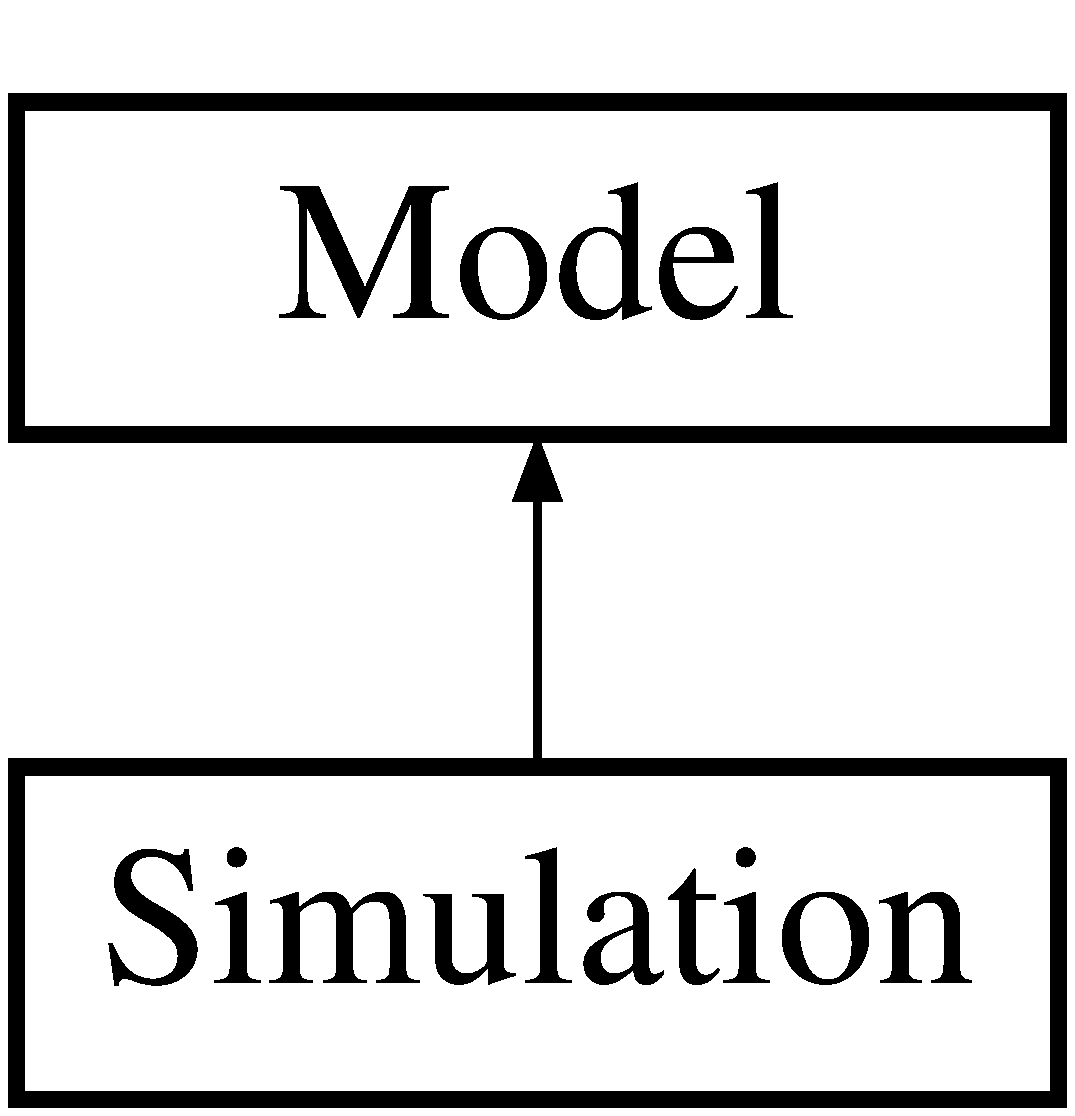
\includegraphics[height=2.000000cm]{structSimulation}
\end{center}
\end{figure}
\subsection*{Public Member Functions}
\begin{DoxyCompactItemize}
\item 
\mbox{\Hypertarget{structSimulation_ae7e550fa89bc4439dc3c90123b068c93}\label{structSimulation_ae7e550fa89bc4439dc3c90123b068c93}} 
int {\bfseries compute\+\_\+spectral\+\_\+discretisation} ()
\item 
\mbox{\Hypertarget{structSimulation_a0c63659d07e5bc9a8dcb8c675e8d1944}\label{structSimulation_a0c63659d07e5bc9a8dcb8c675e8d1944}} 
int {\bfseries compute\+\_\+boundary\+\_\+intensities} ()
\item 
\mbox{\Hypertarget{structSimulation_a36998d85e140ba7f7e7ceb0ea7f1ba80}\label{structSimulation_a36998d85e140ba7f7e7ceb0ea7f1ba80}} 
int \mbox{\hyperlink{structSimulation_a36998d85e140ba7f7e7ceb0ea7f1ba80}{compute\+\_\+radiation\+\_\+field}} ()
\begin{DoxyCompactList}\small\item\em compute\+\_\+radiation\+\_\+field \end{DoxyCompactList}\item 
double \mbox{\hyperlink{structSimulation_a37df96c36c99a3591bb0a7a6f74fa1a1}{get\+\_\+dshift\+\_\+max}} (const long o)
\item 
\mbox{\Hypertarget{structSimulation_aa21d335fc6655ca2f4cc594193df51e0}\label{structSimulation_aa21d335fc6655ca2f4cc594193df51e0}} 
void {\bfseries setup} (const long R, const long origin, const long f, Ray\+Data \&ray\+Data\+\_\+ar, Ray\+Data \&ray\+Data\+\_\+r, \mbox{\hyperlink{structRayPair}{Ray\+Pair}} \&ray\+Pair) const
\item 
\mbox{\Hypertarget{structSimulation_a0cc12a9513e60b8ebec5a01a44c59db3}\label{structSimulation_a0cc12a9513e60b8ebec5a01a44c59db3}} 
void \mbox{\hyperlink{structSimulation_a0cc12a9513e60b8ebec5a01a44c59db3}{get\+\_\+eta\+\_\+and\+\_\+chi}} (const v\+Real \&freq\+\_\+scaled, const long p, long \&lnotch, v\+Real \&eta, v\+Real \&chi) const
\begin{DoxyCompactList}\small\item\em get\+\_\+eta\+\_\+and\+\_\+chi \end{DoxyCompactList}\item 
int \mbox{\hyperlink{structSimulation_a50e59ee3542fc6226ad7dbec52dc8c72}{compute\+\_\+and\+\_\+write\+\_\+image}} (const \mbox{\hyperlink{structIo}{Io}} \&io, const long r)
\item 
\mbox{\Hypertarget{structSimulation_a3049c252acbb537a7f7db6caf59520ec}\label{structSimulation_a3049c252acbb537a7f7db6caf59520ec}} 
int \mbox{\hyperlink{structSimulation_a3049c252acbb537a7f7db6caf59520ec}{compute\+\_\+\+L\+T\+E\+\_\+level\+\_\+populations}} ()
\begin{DoxyCompactList}\small\item\em compute\+\_\+\+L\+T\+E\+\_\+level\+\_\+populations\+: sets level populations to L\+TE values \end{DoxyCompactList}\item 
int \mbox{\hyperlink{structSimulation_a32a1ff3404a290a95b9b3db2cbffba68}{compute\+\_\+level\+\_\+populations}} (const \mbox{\hyperlink{structIo}{Io}} \&io)
\item 
\mbox{\Hypertarget{structSimulation_ae489db8cfd872f168b0dfd3519b3ec11}\label{structSimulation_ae489db8cfd872f168b0dfd3519b3ec11}} 
int \mbox{\hyperlink{structSimulation_ae489db8cfd872f168b0dfd3519b3ec11}{compute\+\_\+level\+\_\+populations\+\_\+opts}} (const \mbox{\hyperlink{structIo}{Io}} \&io, const bool use\+\_\+\+Ng\+\_\+acceleration, const long max\+\_\+niterations)
\begin{DoxyCompactList}\small\item\em compute\+\_\+level\+\_\+populations \end{DoxyCompactList}\item 
void \mbox{\hyperlink{structSimulation_a8f68d28f188303845cab9e16f8512819}{calc\+\_\+\+Jeff}} ()
\end{DoxyCompactItemize}
\subsection*{Public Attributes}
\begin{DoxyCompactItemize}
\item 
\mbox{\Hypertarget{structSimulation_a8f1af666ff7c205e94e555a799f51184}\label{structSimulation_a8f1af666ff7c205e94e555a799f51184}} 
Double1 {\bfseries error\+\_\+max}
\item 
\mbox{\Hypertarget{structSimulation_a794b5063c84238e4fd563f58830b528b}\label{structSimulation_a794b5063c84238e4fd563f58830b528b}} 
Double1 {\bfseries error\+\_\+mean}
\end{DoxyCompactItemize}


\subsection{Detailed Description}
\mbox{\hyperlink{structSimulation}{Simulation}}\+: 

\subsection{Member Function Documentation}
\mbox{\Hypertarget{structSimulation_a8f68d28f188303845cab9e16f8512819}\label{structSimulation_a8f68d28f188303845cab9e16f8512819}} 
\index{Simulation@{Simulation}!calc\+\_\+\+Jeff@{calc\+\_\+\+Jeff}}
\index{calc\+\_\+\+Jeff@{calc\+\_\+\+Jeff}!Simulation@{Simulation}}
\subsubsection{\texorpdfstring{calc\+\_\+\+Jeff()}{calc\_Jeff()}}
{\footnotesize\ttfamily void Simulation\+::calc\+\_\+\+Jeff (\begin{DoxyParamCaption}{ }\end{DoxyParamCaption})}

calc\+\_\+\+J\+\_\+eff\+: calculate the effective mean intensity in a line 
\begin{DoxyParams}[1]{Parameters}
\mbox{\tt in}  & {\em p} & number of the cell under consideration \\
\hline
\mbox{\tt in}  & {\em l} & number of the line producing species under consideration \\
\hline
\end{DoxyParams}
\mbox{\Hypertarget{structSimulation_a50e59ee3542fc6226ad7dbec52dc8c72}\label{structSimulation_a50e59ee3542fc6226ad7dbec52dc8c72}} 
\index{Simulation@{Simulation}!compute\+\_\+and\+\_\+write\+\_\+image@{compute\+\_\+and\+\_\+write\+\_\+image}}
\index{compute\+\_\+and\+\_\+write\+\_\+image@{compute\+\_\+and\+\_\+write\+\_\+image}!Simulation@{Simulation}}
\subsubsection{\texorpdfstring{compute\+\_\+and\+\_\+write\+\_\+image()}{compute\_and\_write\_image()}}
{\footnotesize\ttfamily int Simulation\+::compute\+\_\+and\+\_\+write\+\_\+image (\begin{DoxyParamCaption}\item[{const \mbox{\hyperlink{structIo}{Io}} \&}]{io,  }\item[{const long}]{r }\end{DoxyParamCaption})}

compute\+\_\+and\+\_\+write\+\_\+image\+: 
\begin{DoxyParams}[1]{Parameters}
\mbox{\tt in}  & {\em io} & \+: io object used to write the images \\
\hline
\mbox{\tt in}  & {\em r} & \+: number of the ray indicating the direction of the image \\
\hline
\end{DoxyParams}
\mbox{\Hypertarget{structSimulation_a32a1ff3404a290a95b9b3db2cbffba68}\label{structSimulation_a32a1ff3404a290a95b9b3db2cbffba68}} 
\index{Simulation@{Simulation}!compute\+\_\+level\+\_\+populations@{compute\+\_\+level\+\_\+populations}}
\index{compute\+\_\+level\+\_\+populations@{compute\+\_\+level\+\_\+populations}!Simulation@{Simulation}}
\subsubsection{\texorpdfstring{compute\+\_\+level\+\_\+populations()}{compute\_level\_populations()}}
{\footnotesize\ttfamily int Simulation\+::compute\+\_\+level\+\_\+populations (\begin{DoxyParamCaption}\item[{const \mbox{\hyperlink{structIo}{Io}} \&}]{io }\end{DoxyParamCaption})}

compute\+\_\+level\+\_\+populations\+: computes level populations self-\/consistenly with the radiation field assuming statistical equilibrium \mbox{\Hypertarget{structSimulation_a37df96c36c99a3591bb0a7a6f74fa1a1}\label{structSimulation_a37df96c36c99a3591bb0a7a6f74fa1a1}} 
\index{Simulation@{Simulation}!get\+\_\+dshift\+\_\+max@{get\+\_\+dshift\+\_\+max}}
\index{get\+\_\+dshift\+\_\+max@{get\+\_\+dshift\+\_\+max}!Simulation@{Simulation}}
\subsubsection{\texorpdfstring{get\+\_\+dshift\+\_\+max()}{get\_dshift\_max()}}
{\footnotesize\ttfamily double Simulation\+::get\+\_\+dshift\+\_\+max (\begin{DoxyParamCaption}\item[{const long}]{o }\end{DoxyParamCaption})\hspace{0.3cm}{\ttfamily [inline]}}

get\+\_\+dshift\+\_\+max\+: the maximum allowed shift is determined by the smallest line 
\begin{DoxyParams}[1]{Parameters}
\mbox{\tt in}  & {\em o} & number of point under consideration \\
\hline
\end{DoxyParams}


The documentation for this struct was generated from the following files\+:\begin{DoxyCompactItemize}
\item 
/home/frederik/\+Dropbox/\+Astro/\+Magritte/src/\+Simulation/simulation.\+hpp\item 
/home/frederik/\+Dropbox/\+Astro/\+Magritte/src/\+Simulation/simulation.\+cpp\end{DoxyCompactItemize}

\hypertarget{structSpecies}{}\section{Species Struct Reference}
\label{structSpecies}\index{Species@{Species}}
\subsection*{Public Member Functions}
\begin{DoxyCompactItemize}
\item 
int \mbox{\hyperlink{structSpecies_a8816c98e9fdc90c4b8c8aba44859cc44}{read}} (const \mbox{\hyperlink{structIo}{Io}} \&io, \mbox{\hyperlink{classParameters}{Parameters}} \&parameters)
\item 
int \mbox{\hyperlink{structSpecies_a139fe7d058d5eb90e018b0ebd841d107}{write}} (const \mbox{\hyperlink{structIo}{Io}} \&io) const
\item 
\mbox{\Hypertarget{structSpecies_a4bad6ba4f4074d87721c882532f56067}\label{structSpecies_a4bad6ba4f4074d87721c882532f56067}} 
long {\bfseries get\+\_\+species\+\_\+nr} (const string name) const
\end{DoxyCompactItemize}
\subsection*{Public Attributes}
\begin{DoxyCompactItemize}
\item 
\mbox{\Hypertarget{structSpecies_ab1d965b850c92403ab8475ea2b0068bf}\label{structSpecies_ab1d965b850c92403ab8475ea2b0068bf}} 
String1 \mbox{\hyperlink{structSpecies_ab1d965b850c92403ab8475ea2b0068bf}{sym}}
\begin{DoxyCompactList}\small\item\em chemical symbol of species \end{DoxyCompactList}\item 
\mbox{\Hypertarget{structSpecies_a3df04d380fd2f0a1f8464562c7ad05a0}\label{structSpecies_a3df04d380fd2f0a1f8464562c7ad05a0}} 
Double2 \mbox{\hyperlink{structSpecies_a3df04d380fd2f0a1f8464562c7ad05a0}{abundance\+\_\+init}}
\begin{DoxyCompactList}\small\item\em abundance before chemical evolution \end{DoxyCompactList}\item 
\mbox{\Hypertarget{structSpecies_aa5af9ae841da2d671532d58cd0c84023}\label{structSpecies_aa5af9ae841da2d671532d58cd0c84023}} 
Double2 \mbox{\hyperlink{structSpecies_aa5af9ae841da2d671532d58cd0c84023}{abundance}}
\begin{DoxyCompactList}\small\item\em (current) abundance in every cell \end{DoxyCompactList}\item 
\mbox{\Hypertarget{structSpecies_aab1181ae5af5a0a4904a647f50325465}\label{structSpecies_aab1181ae5af5a0a4904a647f50325465}} 
long {\bfseries nr\+\_\+e}
\item 
\mbox{\Hypertarget{structSpecies_a0464234d60c9a33fa91cb15e627e08d5}\label{structSpecies_a0464234d60c9a33fa91cb15e627e08d5}} 
long {\bfseries nr\+\_\+\+H2}
\item 
\mbox{\Hypertarget{structSpecies_aa132e3fcdfda6783636d831c5275024b}\label{structSpecies_aa132e3fcdfda6783636d831c5275024b}} 
long {\bfseries nr\+\_\+\+HD}
\end{DoxyCompactItemize}


\subsection{Member Function Documentation}
\mbox{\Hypertarget{structSpecies_a8816c98e9fdc90c4b8c8aba44859cc44}\label{structSpecies_a8816c98e9fdc90c4b8c8aba44859cc44}} 
\index{Species@{Species}!read@{read}}
\index{read@{read}!Species@{Species}}
\subsubsection{\texorpdfstring{read()}{read()}}
{\footnotesize\ttfamily int Species\+::read (\begin{DoxyParamCaption}\item[{const \mbox{\hyperlink{structIo}{Io}} \&}]{io,  }\item[{\mbox{\hyperlink{classParameters}{Parameters}} \&}]{parameters }\end{DoxyParamCaption})}

read\+: read the input into the data structure 
\begin{DoxyParams}[1]{Parameters}
\mbox{\tt in}  & {\em io} & io object \\
\hline
\mbox{\tt in}  & {\em parameters} & model parameters object \\
\hline
\end{DoxyParams}
\mbox{\Hypertarget{structSpecies_a139fe7d058d5eb90e018b0ebd841d107}\label{structSpecies_a139fe7d058d5eb90e018b0ebd841d107}} 
\index{Species@{Species}!write@{write}}
\index{write@{write}!Species@{Species}}
\subsubsection{\texorpdfstring{write()}{write()}}
{\footnotesize\ttfamily int Species\+::write (\begin{DoxyParamCaption}\item[{const \mbox{\hyperlink{structIo}{Io}} \&}]{io }\end{DoxyParamCaption}) const}

write\+: write out the data structure 
\begin{DoxyParams}[1]{Parameters}
\mbox{\tt in}  & {\em io} & io object \\
\hline
\end{DoxyParams}


The documentation for this struct was generated from the following files\+:\begin{DoxyCompactItemize}
\item 
/home/frederik/\+Dropbox/\+Astro/\+Magritte/src/\+Model/\+Chemistry/\+Species/species.\+hpp\item 
/home/frederik/\+Dropbox/\+Astro/\+Magritte/src/\+Model/\+Chemistry/\+Species/species.\+cpp\end{DoxyCompactItemize}

\hypertarget{structTemperature}{}\section{Temperature Struct Reference}
\label{structTemperature}\index{Temperature@{Temperature}}
\subsection*{Public Member Functions}
\begin{DoxyCompactItemize}
\item 
int \mbox{\hyperlink{structTemperature_a397a564f10a59b921ff8db065eedd2fc}{read}} (const \mbox{\hyperlink{structIo}{Io}} \&io, \mbox{\hyperlink{classParameters}{Parameters}} \&parameters)
\item 
int \mbox{\hyperlink{structTemperature_a7ad317e6e3ef56b24c628bc838b2ac4e}{write}} (const \mbox{\hyperlink{structIo}{Io}} \&io) const
\end{DoxyCompactItemize}
\subsection*{Public Attributes}
\begin{DoxyCompactItemize}
\item 
\mbox{\Hypertarget{structTemperature_a4a6bee795a4871a93b8e66445d4ae177}\label{structTemperature_a4a6bee795a4871a93b8e66445d4ae177}} 
Double1 \mbox{\hyperlink{structTemperature_a4a6bee795a4871a93b8e66445d4ae177}{gas}}
\begin{DoxyCompactList}\small\item\em \mbox{[}K\mbox{]} gas temperature \end{DoxyCompactList}\end{DoxyCompactItemize}


\subsection{Member Function Documentation}
\mbox{\Hypertarget{structTemperature_a397a564f10a59b921ff8db065eedd2fc}\label{structTemperature_a397a564f10a59b921ff8db065eedd2fc}} 
\index{Temperature@{Temperature}!read@{read}}
\index{read@{read}!Temperature@{Temperature}}
\subsubsection{\texorpdfstring{read()}{read()}}
{\footnotesize\ttfamily int Temperature\+::read (\begin{DoxyParamCaption}\item[{const \mbox{\hyperlink{structIo}{Io}} \&}]{io,  }\item[{\mbox{\hyperlink{classParameters}{Parameters}} \&}]{parameters }\end{DoxyParamCaption})}

read\+: read in data structure 
\begin{DoxyParams}[1]{Parameters}
\mbox{\tt in}  & {\em io} & io object \\
\hline
\mbox{\tt in}  & {\em parameters} & model parameters object \\
\hline
\end{DoxyParams}
\mbox{\Hypertarget{structTemperature_a7ad317e6e3ef56b24c628bc838b2ac4e}\label{structTemperature_a7ad317e6e3ef56b24c628bc838b2ac4e}} 
\index{Temperature@{Temperature}!write@{write}}
\index{write@{write}!Temperature@{Temperature}}
\subsubsection{\texorpdfstring{write()}{write()}}
{\footnotesize\ttfamily int Temperature\+::write (\begin{DoxyParamCaption}\item[{const \mbox{\hyperlink{structIo}{Io}} \&}]{io }\end{DoxyParamCaption}) const}

write\+: write out data structure 
\begin{DoxyParams}[1]{Parameters}
\mbox{\tt in}  & {\em io} & io object \\
\hline
\end{DoxyParams}


The documentation for this struct was generated from the following files\+:\begin{DoxyCompactItemize}
\item 
/home/frederik/\+Dropbox/\+Astro/\+Magritte/src/\+Model/\+Thermodynamics/\+Temperature/temperature.\+hpp\item 
/home/frederik/\+Dropbox/\+Astro/\+Magritte/src/\+Model/\+Thermodynamics/\+Temperature/temperature.\+cpp\end{DoxyCompactItemize}

\hypertarget{structThermodynamics}{}\section{Thermodynamics Struct Reference}
\label{structThermodynamics}\index{Thermodynamics@{Thermodynamics}}
\subsection*{Public Member Functions}
\begin{DoxyCompactItemize}
\item 
int \mbox{\hyperlink{structThermodynamics_a995e360022e63d572760d3a694814fda}{read}} (const \mbox{\hyperlink{structIo}{Io}} \&io, \mbox{\hyperlink{classParameters}{Parameters}} \&parameters)
\item 
int \mbox{\hyperlink{structThermodynamics_ac3f2f42f51d687a833b278723da9460f}{write}} (const \mbox{\hyperlink{structIo}{Io}} \&io) const
\item 
\mbox{\Hypertarget{structThermodynamics_a742d561124ffa6e3eb62aeb56ea64e0d}\label{structThermodynamics_a742d561124ffa6e3eb62aeb56ea64e0d}} 
v\+Real {\bfseries profile} (const double width, const v\+Real freq\+\_\+diff) const
\item 
\mbox{\Hypertarget{structThermodynamics_a4225e85589c6859c4870dad0753a4374}\label{structThermodynamics_a4225e85589c6859c4870dad0753a4374}} 
v\+Real {\bfseries profile} (const double inverse\+\_\+mass, const long p, const double freq\+\_\+line, const v\+Real freq) const
\item 
\mbox{\Hypertarget{structThermodynamics_a4be5974c0bbfdaacd0fe84eb42f02dcd}\label{structThermodynamics_a4be5974c0bbfdaacd0fe84eb42f02dcd}} 
double {\bfseries profile\+\_\+width} (const double inverse\+\_\+mass, const long p, const double freq\+\_\+line) const
\item 
\mbox{\Hypertarget{structThermodynamics_ad7b933687c4161efba31ee6f2c46e74d}\label{structThermodynamics_ad7b933687c4161efba31ee6f2c46e74d}} 
double {\bfseries profile\+\_\+width} (const double inverse\+\_\+mass, const long p) const
\end{DoxyCompactItemize}
\subsection*{Public Attributes}
\begin{DoxyCompactItemize}
\item 
\mbox{\Hypertarget{structThermodynamics_a1165840a9afba6fd0c9b2900233a781f}\label{structThermodynamics_a1165840a9afba6fd0c9b2900233a781f}} 
\mbox{\hyperlink{structTemperature}{Temperature}} {\bfseries temperature}
\item 
\mbox{\Hypertarget{structThermodynamics_a22fc4dfe5e65270192f7a3a78839b480}\label{structThermodynamics_a22fc4dfe5e65270192f7a3a78839b480}} 
\mbox{\hyperlink{structTurbulence}{Turbulence}} {\bfseries turbulence}
\end{DoxyCompactItemize}


\subsection{Member Function Documentation}
\mbox{\Hypertarget{structThermodynamics_a995e360022e63d572760d3a694814fda}\label{structThermodynamics_a995e360022e63d572760d3a694814fda}} 
\index{Thermodynamics@{Thermodynamics}!read@{read}}
\index{read@{read}!Thermodynamics@{Thermodynamics}}
\subsubsection{\texorpdfstring{read()}{read()}}
{\footnotesize\ttfamily int Thermodynamics\+::read (\begin{DoxyParamCaption}\item[{const \mbox{\hyperlink{structIo}{Io}} \&}]{io,  }\item[{\mbox{\hyperlink{classParameters}{Parameters}} \&}]{parameters }\end{DoxyParamCaption})}

read\+: read in data structure 
\begin{DoxyParams}[1]{Parameters}
\mbox{\tt in}  & {\em io} & io object \\
\hline
\mbox{\tt in}  & {\em parameters} & model parameters object \\
\hline
\end{DoxyParams}
\mbox{\Hypertarget{structThermodynamics_ac3f2f42f51d687a833b278723da9460f}\label{structThermodynamics_ac3f2f42f51d687a833b278723da9460f}} 
\index{Thermodynamics@{Thermodynamics}!write@{write}}
\index{write@{write}!Thermodynamics@{Thermodynamics}}
\subsubsection{\texorpdfstring{write()}{write()}}
{\footnotesize\ttfamily int Thermodynamics\+::write (\begin{DoxyParamCaption}\item[{const \mbox{\hyperlink{structIo}{Io}} \&}]{io }\end{DoxyParamCaption}) const}

write\+: write out data structure 
\begin{DoxyParams}[1]{Parameters}
\mbox{\tt in}  & {\em io} & io object \\
\hline
\end{DoxyParams}


The documentation for this struct was generated from the following files\+:\begin{DoxyCompactItemize}
\item 
/home/frederik/\+Dropbox/\+Astro/\+Magritte/src/\+Model/\+Thermodynamics/thermodynamics.\+hpp\item 
/home/frederik/\+Dropbox/\+Astro/\+Magritte/src/\+Model/\+Thermodynamics/thermodynamics.\+cpp\end{DoxyCompactItemize}

\hypertarget{classTIMER}{}\section{T\+I\+M\+ER Class Reference}
\label{classTIMER}\index{T\+I\+M\+ER@{T\+I\+M\+ER}}


\mbox{\hyperlink{classTIMER}{T\+I\+M\+ER}}\+: class for precise process timing.  




{\ttfamily \#include $<$timer.\+hpp$>$}

\subsection*{Public Member Functions}
\begin{DoxyCompactItemize}
\item 
\mbox{\Hypertarget{classTIMER_ad450210e714b4eb2c825da194fbbe221}\label{classTIMER_ad450210e714b4eb2c825da194fbbe221}} 
\mbox{\hyperlink{classTIMER_ad450210e714b4eb2c825da194fbbe221}{T\+I\+M\+ER}} (const string timer\+\_\+name)
\begin{DoxyCompactList}\small\item\em Constructor for \mbox{\hyperlink{classTIMER}{T\+I\+M\+ER}}. \end{DoxyCompactList}\item 
\mbox{\Hypertarget{classTIMER_ab32c9692daffab03c61dff31994a4948}\label{classTIMER_ab32c9692daffab03c61dff31994a4948}} 
void \mbox{\hyperlink{classTIMER_ab32c9692daffab03c61dff31994a4948}{start}} ()
\begin{DoxyCompactList}\small\item\em start\+: start timer i.\+e. set initial time stamp \end{DoxyCompactList}\item 
\mbox{\Hypertarget{classTIMER_a5ffda48b39188174bbfb287923e8c01e}\label{classTIMER_a5ffda48b39188174bbfb287923e8c01e}} 
void \mbox{\hyperlink{classTIMER_a5ffda48b39188174bbfb287923e8c01e}{stop}} ()
\begin{DoxyCompactList}\small\item\em stop\+: stop timer and calculate interval for every process \end{DoxyCompactList}\item 
\mbox{\Hypertarget{classTIMER_a526fe17e0ba4303230c43b3e5b8e5efe}\label{classTIMER_a526fe17e0ba4303230c43b3e5b8e5efe}} 
void \mbox{\hyperlink{classTIMER_a526fe17e0ba4303230c43b3e5b8e5efe}{print\+\_\+to\+\_\+file}} ()
\begin{DoxyCompactList}\small\item\em print\+\_\+to\+\_\+file\+: print time interval to file \end{DoxyCompactList}\item 
\mbox{\Hypertarget{classTIMER_ad771cc2a3de3cd4535293167e730182d}\label{classTIMER_ad771cc2a3de3cd4535293167e730182d}} 
void \mbox{\hyperlink{classTIMER_ad771cc2a3de3cd4535293167e730182d}{print}} ()
\begin{DoxyCompactList}\small\item\em print\+: print time interval to screen \end{DoxyCompactList}\end{DoxyCompactItemize}


\subsection{Detailed Description}
\mbox{\hyperlink{classTIMER}{T\+I\+M\+ER}}\+: class for precise process timing. 

The documentation for this class was generated from the following file\+:\begin{DoxyCompactItemize}
\item 
/home/frederik/\+Dropbox/\+Astro/\+Magritte/src/\+Tools/timer.\+hpp\end{DoxyCompactItemize}

\hypertarget{structTurbulence}{}\section{Turbulence Struct Reference}
\label{structTurbulence}\index{Turbulence@{Turbulence}}
\subsection*{Public Member Functions}
\begin{DoxyCompactItemize}
\item 
int \mbox{\hyperlink{structTurbulence_a4cb9c16ae37770b4873d7ab1b14e0b7f}{read}} (const \mbox{\hyperlink{structIo}{Io}} \&io, \mbox{\hyperlink{classParameters}{Parameters}} \&parameters)
\item 
int \mbox{\hyperlink{structTurbulence_a5552d24c437399f5363d2e1ac97c12af}{write}} (const \mbox{\hyperlink{structIo}{Io}} \&io) const
\end{DoxyCompactItemize}
\subsection*{Public Attributes}
\begin{DoxyCompactItemize}
\item 
\mbox{\Hypertarget{structTurbulence_a75006a6d67857dd02e0f582813838683}\label{structTurbulence_a75006a6d67857dd02e0f582813838683}} 
Double1 \mbox{\hyperlink{structTurbulence_a75006a6d67857dd02e0f582813838683}{vturb2}}
\begin{DoxyCompactList}\small\item\em \mbox{[}.\mbox{]} microturbulence over c all squared \end{DoxyCompactList}\end{DoxyCompactItemize}


\subsection{Member Function Documentation}
\mbox{\Hypertarget{structTurbulence_a4cb9c16ae37770b4873d7ab1b14e0b7f}\label{structTurbulence_a4cb9c16ae37770b4873d7ab1b14e0b7f}} 
\index{Turbulence@{Turbulence}!read@{read}}
\index{read@{read}!Turbulence@{Turbulence}}
\subsubsection{\texorpdfstring{read()}{read()}}
{\footnotesize\ttfamily int Turbulence\+::read (\begin{DoxyParamCaption}\item[{const \mbox{\hyperlink{structIo}{Io}} \&}]{io,  }\item[{\mbox{\hyperlink{classParameters}{Parameters}} \&}]{parameters }\end{DoxyParamCaption})}

read\+: read in data structure 
\begin{DoxyParams}[1]{Parameters}
\mbox{\tt in}  & {\em io} & io object \\
\hline
\mbox{\tt in}  & {\em parameters} & model parameters object \\
\hline
\end{DoxyParams}
\mbox{\Hypertarget{structTurbulence_a5552d24c437399f5363d2e1ac97c12af}\label{structTurbulence_a5552d24c437399f5363d2e1ac97c12af}} 
\index{Turbulence@{Turbulence}!write@{write}}
\index{write@{write}!Turbulence@{Turbulence}}
\subsubsection{\texorpdfstring{write()}{write()}}
{\footnotesize\ttfamily int Turbulence\+::write (\begin{DoxyParamCaption}\item[{const \mbox{\hyperlink{structIo}{Io}} \&}]{io }\end{DoxyParamCaption}) const}

write\+: write out data structure 
\begin{DoxyParams}[1]{Parameters}
\mbox{\tt in}  & {\em io} & io object \\
\hline
\end{DoxyParams}


The documentation for this struct was generated from the following files\+:\begin{DoxyCompactItemize}
\item 
/home/frederik/\+Dropbox/\+Astro/\+Magritte/src/\+Model/\+Thermodynamics/\+Turbulence/turbulence.\+hpp\item 
/home/frederik/\+Dropbox/\+Astro/\+Magritte/src/\+Model/\+Thermodynamics/\+Turbulence/turbulence.\+cpp\end{DoxyCompactItemize}

%--- End generated contents ---

% Index
\backmatter
\newpage
\phantomsection
\clearemptydoublepage
\addcontentsline{toc}{chapter}{Index}
\printindex

\end{document}
